% http://mstracker.com
% Manuscript 12-313-RR
% Dynamic Enforcement of Knowledge-based Security Policies using Probabilistic Abstract Interpretation
% Mr. Piotr Mardziel piotrm@cs.umd.edu USA UMD College Park
% Dr. Stephen Magill stephen.magill@gmail.com USA UMD College Park
% Dr. Michael Hicks mwh@cs.umd.edu USA UMD College Park
% Dr. Mudhakar Srivatsa msrivats@us.ibm.com USA IBM TJ Watson

%\newif \ifdraft \drafttrue
\newif \ifdraft \draftfalse
\newif \iffullapp \fullappfalse

%\documentclass[10pt,conference,compsocconf]{IEEEtran}
\documentclass[9pt]{article}
%\usepackage{times}
\usepackage{times}
\usepackage[hyphens]{url}
\usepackage{amssymb}
\usepackage{color}
\usepackage{amsthm}
\usepackage{amsmath}
\usepackage{bigstrut}
%\usepackage{alg}
\usepackage[override]{cmtt}
\usepackage[nointegrals]{wasysym}
\usepackage{graphicx}
\usepackage{balance}
\usepackage{longtable}

%%% names
\newcommand{\flowcheck}{\textsc{FlowCheck}}
\newcommand{\parma}{PARMA}

\makeatletter
\newtheorem*{rep@theorem}{\rep@title}
\newcommand{\newreptheorem}[2]{%
\newenvironment{rep#1}[1]{%
 \def\rep@title{#2 \ref{##1}}%
 \begin{rep@theorem}}%
 {\end{rep@theorem}}}
\makeatother

\theoremstyle{plain} % bold head, italicized body  (the default)
\newtheorem{theorem}{Theorem}
\newreptheorem{theorem}{Theorem}
\newtheorem{lemma}[theorem]{Lemma}
\newreptheorem{lemma}{Lemma}
\newtheorem{proposition}[theorem]{Proposition}
\newtheorem{corollary}[theorem]{Corollary}
\newtheorem{axiom}{Axiom}

\newcounter{subtheorem}[theorem]
\newtheorem{subtheorem}[subtheorem]{}
\renewcommand{\thesubtheorem}{\thetheorem{} (\roman{subtheorem})}

% https://secure.wikimedia.org/wikibooks/en/wiki/LaTeX/Theorems
% Fix latex
\def\smallskip{\vskip\smallskipamount}
\def\medskip{\vskip\medskipamount}
\def\bigskip{\vskip\bigskipamount}
 
% Hand made theorem
\def\subtheorem{%
\par\smallskip\indent\refstepcounter{subtheorem}\hbox{\bf%
    (\roman{subtheorem})}%
\it\ %\ignorespaces
}
\def\endsubtheorem{\par\smallskip}
\newenvironment{thm}{\subtheorem}{\endsubtheorem}

\def\subproof#1{%
\par\smallskip\noindent\hbox{{\em} \bf%
    #1.}%
\ %\ignorespaces
}
\def\endsubproof{\qed\par\smallskip}
\newenvironment{subproofe}{\subproof}{\endsubproof}



\theoremstyle{definition} % bold head, normal body
\newtheorem{definition}[theorem]{Definition}
\newtheorem*{definition-un}{Definition}
\newtheorem{notation}[theorem]{Notation}
\newtheorem*{notation-un}{Notation}
\newtheorem{remark}[theorem]{Remark}
\newtheorem*{remark-un}{Remark}
\newtheorem*{claim}{Claim}

\theoremstyle{remark} % italic head, normal body
\newtheorem{example}[theorem]{Example}
\newtheorem*{example-un}{Example}
\newtheorem{examples}[theorem]{Examples}
\newtheorem*{examples-un}{Examples}
\newtheorem*{hint}{Hint}

\newcommand{\imp}{\Rightarrow}
\newcommand{\ybox}[1]{\parbox{5.5in}{\vspace{0.1in} \hl{#1} \vspace{0.1in}}}
\newcommand{\note}[1]{{\textbf{Note: #1}}}
% \newcommand{\todo}[1]{{\color{red}{\textbf{To do:} #1}}}
% \newcommand{\goal}[1]{\ybox{\textbf{Goal}: #1}}
% \newcommand{\activity}[1]{\ybox{\textbf{Research activity}: #1}}
% \newcommand{\problem}[1]{\ybox{\textbf{Research problem}: #1}}
% \newcommand{\question}[1]{\ybox{\textbf{Question}: #1}}

\newcommand{\stacklabel}[1]{\stackrel{\smash{\scriptscriptstyle \mathrm{#1}}}}
\newcommand{\defeq}{\stacklabel{def}=}
\newcommand{\nzset}[1]{\textit{support}(#1)}
\newcommand{\support}[1]{\nzset{#1}}
\newcommand{\overlap}[2]{\textit{overlap}(#1,#2)}
\newcommand{\cp}{\mathbb{C}}
% deleted \ppbot, use \ppzero instead
\newcommand{\pconcfun}{\gamma_{\cp}}
\newcommand{\pconc}[1]{\gamma_{\cp}(#1)}
\newcommand{\psconc}[1]{\gamma_{\powersetb{}{\cp}}(#1)}
\newcommand{\ppconcfun}{\gamma_{\ppolys}}
\newcommand{\ppsconcfun}{\gamma_{\ppowers}}
\newcommand{\ppconc}[1]{\ppconcfun(#1)}
\newcommand{\ppowers}[0]{\powersetb{n}{\ppolys}}
\newcommand{\ppsconc}[1]{\ppsconcfun(#1)}

\newcommand{\abst}[1]{\alpha(#1)}
\newcommand{\lub}[1]{\textit{lub}(#1)}
\newcommand{\glb}[1]{\textit{glb}(#1)}
\newcommand{\chull}[1]{\textit{chull}(#1)}
\newcommand{\dom}[1]{\textit{domain}(#1)}
\newcommand{\fv}[1]{\textit{fv}(#1)}

\newcommand{\var}[1]{\ensuremath{\mathit{#1}}}
\newcommand{\aif}[0]{\text{ \textbf{if} }}
\newcommand{\aendif}[0]{\text{ \textbf{endif} }}
\newcommand{\apif}[0]{\text{ \textbf{pif} }}
\newcommand{\athen}[0]{\text{ \textbf{then} }}
\newcommand{\aelse}[0]{\text{ \textbf{else} }}
\newcommand{\aendpif}[0]{\text{ \textbf{endpif} }}
\newcommand{\atrue}[0]{\text{ \textbf{true} }}
\newcommand{\afalse}[0]{\text{ \textbf{false} }}
\newcommand{\aor}[0]{\text{ \textbf{or} }}
\newcommand{\aand}[0]{\text{ \textbf{and} }}
\newcommand{\asemi}[0]{\text{ \textbf{;} }}
\newcommand{\aassign}[0]{\text{ \textbf{=} }}
\newcommand{\askip}[0]{\text{ \textbf{skip} }}
\newcommand{\aneg}[1]{\neg #1}

\newcommand{\sconst}[1]{\ensuremath{\mathsf{#1}}}
\newcommand{\strue}{\sconst{True}}
\newcommand{\sfalse}{\sconst{False}}
\newcommand{\sskip}{\mathsf{skip}}
\newcommand{\sifk}{\mathsf{if}}
\newcommand{\spifk}{\mathsf{pif}}
\newcommand{\sthenk}{\mathsf{then}}
\newcommand{\selsek}{\mathsf{else}}
\newcommand{\sif}[3]{\sifk\;{#1}\;\sthenk\;{#2}\;\mathsf{else}\;{#3}}
\newcommand{\sifnoelse}[2]{\sifk\;{#1}\;\sthenk\;{#2}}
\newcommand{\spif}[3]{\spifk\;{#1}\;\sthenk\;{#2}\;\mathsf{else}\;{#3}}
\newcommand{\spifnoelse}[2]{\spifk\;{#1}\;\sthenk\;{#2}}
\newcommand{\sassign}[2]{{#1}\;:=\;{#2}}
\newcommand{\sseq}[2]{{#1} \;;\; {#2}}
\newcommand{\swhile}[2]{\mathsf{while}\;{#1}\;\mathsf{do}\;{#2}}
\newcommand{\suniformname}[0]{\mathsf{uniform}}
\newcommand{\suniform}[3]{\suniformname\;{#1}\;{#2}\;#3}
\newcommand{\ebinop}[3]{#2 #1 #3}
\newcommand{\ssecretk}{\mathsf{secret}}
\newcommand{\sbeliefk}{\mathsf{belief}}
\newcommand{\squerydefk}{\mathsf{querydef}}
\newcommand{\squeryk}{\mathsf{query}}

\newcommand{\stmt}{\mathit{S}}
\newcommand{\aexp}{\mathit{E}}
\newcommand{\bexp}{\mathit{B}}
\newcommand{\relop}{\mathit{relop}}
\newcommand{\arithop}{\mathit{aop}}
\newcommand{\aop}[2]{#1\;\arithop\;#2}
\newcommand{\bop}[2]{#1 \;\relop\; #2}

\newcommand{\vars}[0]{\textbf{Var}}
\newcommand{\states}[0]{\textbf{State}}
\newcommand{\dists}[0]{\textbf{Dist}}
\newcommand{\vals}[0]{\textbf{Val}}
\newcommand{\pmass}[1]{\mathord{\parallel}#1\mathord{\parallel}}
\newcommand{\normal}[1]{\text{normal}(#1)}

\newcommand{\sem}[2]{[\![{#1}]\!]{#2}}
\newcommand{\eeval}[2]{[\![{#1}]\!]{#2}}
\newcommand{\eval}[2]{[\![{#1}]\!]{#2}}
\newcommand{\evalp}[2]{[\![{#1}]\!]{#2}}
\newcommand{\pevalp}[2]{[\![{#1}]\!]{#2}}

\newcommand{\ssplit}[1]{\text{ssplit}\paren{#1}}

\newcommand{\sor}[0]{\;|\;}

\newcommand{\polypoint}[1]{\hat{#1}}

\newcommand{\absbexp}[1]{a(#1)}
\newcommand{\absdbexp}[2]{a^{#1}(#2)}

\newcommand{\auniform}[0]{\text{ \textbf{uniform} }}

\newcommand{\repart}[1]{repart\paren{#1}}

\newcommand{\vkill}{\vspace{-10pt plus 5pt minus 5pt}}

%%% groupings
\newcommand{\ceil}[1]{\lceil #1 \rceil}
\newcommand{\floor}[1]{\lfloor #1 \rfloor}
\newcommand{\paren}[1]{\left( #1 \right)}
\newcommand{\bparen}[1]{\left[ #1 \right]}
\newcommand{\aparen}[1]{\langle #1 \rangle}
\newcommand{\tparen}[1]{\bigl( #1 \bigr)}
\newcommand{\sparen}[1]{\left\{ #1 \right\}}
\newcommand{\maxparen}[1]{\max\sparen{#1}}
\newcommand{\minparen}[1]{\min\sparen{#1}}

%%% logic
\newcommand{\lequiv}[0]{\vdash \dashv}
\newcommand{\limp}{\Rightarrow}
\newcommand{\lh}[1]{lh\paren{#1}}
\newcommand{\lps}[1]{p_l\left[#1\right]}
\newcommand{\rps}[1]{p_r\left[#1\right]}
\newcommand{\ass}[1]{h\paren{#1}}
\newcommand{\assb}[1]{\bar{h}\paren{#1}}
\newcommand{\ra}{\rightarrow}
\newcommand{\lra}{\leftrightarrow}
\newcommand{\sA}{\mathfrak{A}}
\newcommand{\sAA}{\mathfrak{A}_A}
\newcommand{\sB}{\mathfrak{B}}
\newcommand{\sBB}{\mathfrak{B}_B}
\newcommand{\sC}{\mathfrak{C}}
\newcommand{\sCC}{\mathfrak{C}_C}
\newcommand{\sD}{\mathfrak{D}}
\newcommand{\sDD}{\mathfrak{D}_D}
\newcommand{\sN}{\mathfrak{N}}
\newcommand{\sNN}{\mathfrak{N}_N}
\newcommand{\Cn}[1]{Cn\paren{#1}}
\newcommand{\Th}[1]{Th\paren{#1}}
\newcommand{\sents}[0]{Sn_L}
\newcommand{\forms}[0]{Fm_L}

\newcommand{\lsep}[0]{. \;}
\newcommand{\qsep}[0]{\; . \;}

%%% number sets
\newcommand{\Natural}{\mathbb{N}}
\newcommand{\Integer}{\mathbb{Z}}
\newcommand{\Rational}{\mathbb{Q}}
\newcommand{\Real}{\mathbb{R}}
\newcommand{\Complex}{\mathbb{C}}

%%% misc
\newcommand{\logtwo}[1]{\lg \left( #1 \right)}
\newcommand{\abs}[1]{\left| #1 \right|}

%%% referencing
\newcommand{\aref}[1]{Axiom \ref{#1}}
\newcommand{\alref}[1]{Algorithm \ref{#1}}
\newcommand{\apref}[1]{Appendix \ref{#1}}
\newcommand{\pref}[1]{Proposition \ref{#1}}
\newcommand{\eref}[1]{Example \ref{#1}}
\newcommand{\fref}[1]{Figure \ref{#1}}
\newcommand{\sref}[1]{Section \ref{#1}}
\newcommand{\rref}[1]{Remark \ref{#1}}
\newcommand{\dref}[1]{Definition \ref{#1}}
\newcommand{\tref}[1]{Theorem \ref{#1}}
\newcommand{\lref}[1]{Lemma \ref{#1}}
\newcommand{\cref}[1]{Condition \cnumref{#1}}
\newcommand{\cnumref}[1]{(\ref{#1})}
\newcommand{\clref}[1]{Claim \cnumref{#1}}


%%% sets
\newcommand{\powerset}[1]{\mathcal{P}\paren{#1}}
\newcommand{\powersetb}[2]{\mathcal{P}_{#1}\paren{#2}}
\newcommand{\set}[1]{\left\{ #1 \right\}}
\newcommand{\setsize}[1]{\left| #1 \right|}
\newcommand{\vect}[1]{\langle #1 \rangle}
\newcommand{\irange}[2]{\set{#1, ..., #2}}
\newcommand{\ssupset}[1]{#1^{+}}
\newcommand{\ssubset}[1]{#1^{-}}

%%% probabilities and moments
\newcommand{\Prob}[1]{\textbf{Pr}\left[#1\right]}
\newcommand{\Expect}[1]{E \left[ #1 \right]}
\newcommand{\Var}[1]{Var \left[ #1 \right]}
\newcommand{\Covar}[2]{Cov \left[ #1, #2 \right]}
\newcommand{\given}{\;|\;}

%%% operations on distributions
\newcommand{\dcond}[2]{#1 | #2}
\newcommand{\pmassmax}[1]{\mathord{\parallel}#1\mathord{\parallel}^\text{max}}
\newcommand{\pmassmin}[1]{\mathord{\parallel}#1\mathord{\parallel}^\text{min}}

%%% probabilistic polyhedra
\newcommand{\maxprobof}[2]{\overline{#1}(#2)}

\newcommand{\ppname}{probabilistic polyhedron}
\newcommand{\ppnames}{probabilistic polyhedra}
\newcommand{\ppsname}{\ppname{} set}
\newcommand{\ppsnames}{\ppname{} sets}
%\newcommand{\pcup}{\mathrel{\vcenter{\offinterlineskip\hbox{\scriptsize$\hspace*{0.1ex}\mathord{+}$}\vskip-1ex\hbox{$\sqcup$}}}}
%\newcommand{\pcap}{\sqcap}
\newcommand{\poly}{C}
\newcommand{\cons}{B}
\newcommand{\polyset}{\mathcal{C}}
\newcommand{\ppoly}{P}
\newcommand{\abseeval}[2]{\langle\!\langle{#1}\rangle\!\rangle\,{#2}}
\newcommand{\absecount}[2]{#2 \# #1}
\newcommand{\pmeet}{\sqcap_{\cp}}
\newcommand{\pjoin}{\sqcup_{\cp}}
\newcommand{\dprod}{\times}
\newcommand{\pprod}{\times}
\newcommand{\pord}{\sqsubseteq_{\cp}}
\newcommand{\pleq}{\sqsubseteq_{\cp}}
\newcommand{\ple}{\sqsubset_{\cp}}
\newcommand{\ppord}{\sqsubseteq_{\ppolys}}
\newcommand{\ppleq}{\ppord}
\newcommand{\pple}{\sqsubset_{\ppolys}}
\newcommand{\distleq}{\leq}
\newcommand{\distle}{\le}
\newcommand{\ppcup}{\mathrel{\tilde{\cup}}}
\newcommand{\ppcap}{\mathrel{\tilde{\cap}}}
\newcommand{\emptypoly}{\emptyset_{\polyset}}
\newcommand{\iszero}[1]{\mathit{iszero}(#1)}
\newcommand{\isempty}[1]{\mathit{isempty}(#1)}
\newcommand{\pa}[0]{\poly_1}
\newcommand{\pb}[0]{\poly_2}
\newcommand{\pc}[0]{\poly_3}
\newcommand{\pp}[1]{P_{#1}}
\newcommand{\distset}[1]{D_{#1}}
\newcommand{\ppeq}[0]{\equiv}
\newcommand{\ppneq}[0]{{\not \equiv}}
\newcommand{\ppzero}[0]{0_{\ppolys}}
\newcommand{\ppfunzero}[0]{\bot_{\ppolys}}
\newcommand{\distzero}[0]{0_{\dists}}
\newcommand{\distfunzero}[0]{\bot_{\dists}}
\newcommand{\pps}[1]{\Delta_{#1}}
\newcommand{\ppsmax}[1]{max_{pp}\paren{#1}}
\newcommand{\ppolys}{\mathbb{P}}
\newcommand{\ppp}[1]{\getpoly{1}}
\newcommand{\ppa}[0]{\pp{1}}
\newcommand{\ppb}[0]{\pp{2}}
\newcommand{\ppc}[0]{\pp{3}}
\newcommand{\pmin}[1]{\mathrm{p}^\mathrm{min}_{#1}}
\newcommand{\pmax}[1]{\mathrm{p}^\mathrm{max}_{#1}}
\newcommand{\smin}[1]{\mathrm{s}^\mathrm{min}_{#1}}
\newcommand{\smax}[1]{\mathrm{s}^\mathrm{max}_{#1}}
\newcommand{\mmin}[1]{\mathrm{m}^\mathrm{min}_{#1}}
\newcommand{\mmax}[1]{\mathrm{m}^\mathrm{max}_{#1}}
\newcommand{\maxh}[1]{\mathrm{h}^\mathrm{max}_{#1}}
\newcommand{\minh}[1]{\mathrm{h}^\mathrm{min}_{#1}}

\newcommand{\vcomp}[0]{\overline{V}}

\newcommand{\parta}[0]{\mathcal{L}}

\newcommand{\ppprob}[2]{#1^{\text{max}}\paren{#2}}
\newcommand{\ppsprob}[2]{#1^{\text{max}}\paren{#2}}

\newcommand{\ppmmin}[1]{\mathrm{M}^\mathrm{min} (#1)}
\newcommand{\ppmmax}[1]{\mathrm{M}^\mathrm{max} (#1)}

\newcommand{\getpoly}[1]{\poly_{#1}}

% assignment
\newcommand{\bassign}[2]{#1 \ra #2}
\newcommand{\stassign}[3]{#1 \bparen{\bassign{#2}{#3}}}
\newcommand{\stsassign}[3]{#1 \bparen{\bassign{#2}{#3}}}
\newcommand{\funassign}[2]{t_{\bassign{#1}{#2}}}
\newcommand{\funinvassign}[2]{t_{\bassign{#1}{#2}}^{-1}}
\newcommand{\eqassign}[3]{\aparen{#1}^{\bassign{#2}{#3}}}
\newcommand{\eqassignsup}[4]{\aparen{#1}^{\bassign{#2}{#3}}_#4}
\newcommand{\dassign}[3]{#1 \bparen{#2 \ra #3}}
\newcommand{\deassign}[3]{#1 \aparen{#2 \ra #3}}

%\newcommand{\pmin}[1]{\lfloor{\ppoly_#1}\rfloor_\mathrm{p}}
%\newcommand{\pmax}[1]{\lceil{\ppoly_#1}\rceil^\mathrm{p}}
%\newcommand{\smin}[1]{\lfloor{\ppoly_#1}\rfloor_\mathrm{s}}
%\newcommand{\smax}[1]{\lceil{\ppoly_#1}\rceil^\mathrm{s}}
%\newcommand{\mmin}[1]{\lfloor{\ppoly_#1}\rfloor_\mathrm{m}}
%\newcommand{\mmax}[1]{\lceil{\ppoly_#1}\rceil^\mathrm{m}}
%\newcommand{\getpoly}[1]{\pentagon{#1}}
\newcommand{\psize}[1]{\#(#1)}
\newcommand{\phull}[1]{hull\paren{#1}}
\newcommand{\pinter}[2]{#1 \cap #2}
\newcommand{\ppplus}{+}
\newcommand{\pessoverlap}[2]{#1 \mathrel{\frownie} #2}
\newcommand{\optoverlap}[2]{#1 \mathrel{\smiley} #2}
\newcommand{\abspevalp}[2]{\langle\!\langle{#1}\rangle\!\rangle\,{#2}}
%\newcommand{\absdcond}[2]{#1 \wr #2}
\newcommand{\absdcond}[2]{#1 \mid #2}
\newcommand{\abspolicy}[3]{\mathit{tsecure}_{#3}(#1,#2)}
\newcommand{\abspolicyname}{\mathit{tsecure}}

\newcommand{\simplify}[2]{\floor{#1}_{#2}}
\newcommand{\bigsimplify}[2]{\Bigl\lfloor{#1}\Bigr\rfloor_{#2}}

%%% semantic sets and meta-variables
\newcommand{\Z}{\Integer}
\newcommand{\ineq}{\beta}

\newcommand{\project}[2]{#1 \upharpoonright #2}
\newcommand{\forget}[2]{\mathrm{f}_{#1}(#2)}
%\newcommand{\newdim}[2]{\mathrm{e}_{#1}(#2)}

\newcommand{\deleted}[1]{}

\newcommand{\pcase}[1]{\textsc{case} {#1}: }

%%% for proofs in appendix
\newcommand{\eqclass}[3]{\bparen{#1}_{#2}^{#3}}
\newcommand{\eqclassc}[3]{\overline{\bparen{#1}}_{#2}^{#3}}

\newcommand{\mathstep}[1]{\text{[ #1 ]}}
\newcommand{\lfp}{\mathrm{lfp}}


%\IEEEoverridecommandlockouts
\title{Dynamic Enforcement of Knowledge-based Security Policies using
  Probabilistic Abstract Interpretation}

\author{
Piotr Mardziel$^\dagger$, Stephen Magill, Michael Hicks$^\dagger$, Mudhakar
Srivatsa$^\star$\\\\
$^\dagger$ University of Maryland, College Park\\
$^\star$ IBM T.J. Watson Research Laboratory\\
}

\newcommand{\myparagraph}[1]{\textbf{#1}.}
\ifdraft
\newcommand{\todo}[1]{\textbf{#1}}
\definecolor{purple}{rgb}{0.8,0,0.8}
\definecolor{dgreen}{rgb}{0.0,0.5,0.0}
\newcommand{\sbmcomment}[1]{\textcolor{purple}{SBM -- #1}}
\newcommand{\mwh}[1]{\textcolor{blue}{MWH -- #1}}
\newcommand{\pxm}[1]{\textcolor{red}{PM -- #1}}
\newcommand{\changed}[1]{\textcolor{dgreen}{#1}}
\newcommand{\ms}[1]{\textcolor{yellow}{MS -- #1}}
\else
\newcommand{\changed}[1]{#1}
\newcommand{\todo}[1]{}
\newcommand{\sbmcomment}[1]{}
\newcommand{\mwh}[1]{}
\newcommand{\pxm}[1]{}
\newcommand{\ms}[1]{}
\fi

\begin{document}

\pagestyle{plain}

\maketitle
\date{}

%Piotr Mardziel - University of Maryland, College Park
%Stephen Magill
%Michael Hicks - University of Maryland, College Park
%Mudhakar Srivatsa - IBM T.J. Watson Research Laboratory

\begin{abstract}
% Following Simon PJ (Kent Beck, actually) abstract structure:
% 1. State the problem 
% 2. Say why it’s an interesting problem 
% 3. Say what your solution achieves 
% 4. Say what follows from your solution

  This paper explores the idea of \emph{knowledge-based security
    policies}, which are used to decide whether to answer queries over
    secret data based on an estimation of the querier's (possibly
    increased) knowledge given the results.  Limiting knowledge is the
    goal of existing information release policies that employ
    mechanisms such as noising, anonymization, and redaction.
    Knowledge-based policies are more general: they increase
    flexibility by not fixing the means to restrict information flow.
    We enforce a knowledge-based policy by explicitly tracking a model
    of a querier's belief about secret data, represented as a
    probability distribution, and denying any query that could
    increase knowledge above a given threshold.  We implement query
    analysis and belief tracking via abstract interpretation, which allows us to
    trade off precision and performance through the use of
    abstraction. We have developed an approach to augment standard
    abstract domains to include probabilities, and thus define
    distributions.  We focus on developing \emph{probabilistic
      polyhedra} in particular, to support numeric programs. While
    probabilistic abstract interpretation has been 
    considered before, our domain is the first whose design supports
    sound conditioning, which is required to ensure that estimates of
    a querier's knowledge are accurate. Experiments with our
    implementation show that several useful queries can be handled
    efficiently, particularly compared to exact (i.e., sound)
    inference involving sampling.  We also show that, for our
    benchmarks, restricting constraints to \emph{octagons}
    or \emph{intervals}, rather than full polyhedra, can dramatically
    improve performance while incurring little to no loss in
    precision.
\end{abstract}

\section{Introduction}

% MWH: Changed the first paragraph to reflect these observations: I
% don't believe third-party apps do the targeted ads, Facebook does.
% Also, I don't think we should indicate that Facebook might be trusted.
% We want to lump it with apps as possibly untrusted.  That's what the
% myspace data comment, and the EULA comment, was about.

Facebook, Twitter, Flickr, and other successful on-line services
enable users to easily foster and maintain relationships by sharing
information with friends and fans.  These services store users'
personal information and use it to customize the user experience and
to generate revenue.  For example, Facebook third-party applications
are granted access to a user's ``basic'' data (which includes name,
profile picture, gender, networks, user ID, and list of
friends~\cite{facebook-apps}) to implement services like birthday
announcements and horoscopes, while Facebook selects ads based on age,
gender, and even sexual preference~\cite{guha10}.  Unfortunately, once
personal information is collected, users have limited control over how
it is used.  For example, Facebook's EULA grants Facebook a
non-exclusive license to any content a user posts~\cite{facebook-tos}.
MySpace, another social network site, has begun to sell its
users' data~\cite{myspace-data}.

Some researchers have proposed that, to keep tighter control over
their data, users could use a storage server (e.g., running on their
home network) that handles personal data requests, and only responds
when a request is deemed safe~\cite{prpl,persona}.  The question is:
which requests are safe?
% The standard answer is to defer to some kind of user-determined
% access control policy.
While deferring to user-defined access control policies seems an
obvious approach, such policies are unnecessarily restrictive when the
goal is to maximize the customized personal experience.  To see why,
consider two example applications: a horoscope or ``happy birthday''
application that operates on birth month and day, and a music
recommendation algorithm that considers birth year (age).  Access
control at the granularity of the entire birth date could preclude
both of these applications, while choosing only to release birth year
or birth day precludes access to one application or the other.  But in
fact the user may not care much about these particular bits of
information, but rather about what can be deduced from them.  For
example, it has been reported that zip code, birth date, and gender
are sufficient information to uniquely identify 87\% of Americans in
the 1990 U.S. census \cite{census90} and 63\% in the 2000 census
\cite{golle06revisiting}. So the user may be perfectly happy to reveal
any one of these bits of information as long as a querier gains no
better than a $1 / n$ chance to guess the entire group, for some
parameter $n$.

This paper explores the design and implementation for enforcing what
we call \emph{knowledge-based security policies}.  In our model, a
user $U$'s agent responds to queries involving secret data.  For each
querying principal $Q$, the agent maintains a probability distribution
over $U$'s secret data, representing $Q$'s \emph{belief} of the data's
likely values.  For example, to mediate queries from a social
networking site $X$, user $U$'s agent may model $X$'s otherwise
uninformed knowledge of $U$'s birthday according to a likely
demographic: the birth month and day are uniformly distributed, while
the birth year is most likely between 1956 and
1992~\cite{facebook-demographics}.  Each querier $Q$ is also assigned
a knowledge-based policy, expressed as a set of thresholds, each
applying to a different group of (potentially overlapping) data.  For
example, $U$'s policy for $X$ might be a threshold of $1/100$ for the
entire tuple $(\var{birthdate},\var{zipcode},\var{gender})$, and $1/5$
for just birth date.  $U$'s agent refuses any queries that it
determines could increase $Q$'s ability to guess a secret above the
assigned threshold.  If deemed safe, $U$'s agent returns the query's
(exact) result and updates $Q$'s modeled belief appropriately.
%(We touch upon the risk of colluding queriers shortly.)

Throughout the paper we use users' personal information protection
when interacting with services like Facebook (or its advertisers) as a
running example, but knowledge-based security policies have other
applications as well.  For example, they can be used to decide whether
a principal should participate in a \emph{secure multiparty
  computation} involving multiple principals each with its own
secrets, such as their current location or available resources.  We
have explored this application in some detail in recent
work~\cite{mardziel12smc}.  Knowledge-based policies could also be
used to protect against browser fingerprinting, which aims to uniquely
identify individuals based on environmental indicators visible to
Javascript programs~\cite{boda11fingerprint}. Users could set a
threshold policy over the tuple of the most sensitive indicators, and
prevent the execution of the Javascript program (or execute only a
modified version) if the threshold is exceeded.  Another example would
be application to privacy-preserving smart
metering~\cite{rial11smart}.  Here, the proposal is that rather than
report fine-grained power usage information back to the power company,
which could compromise privacy, the pricing algorithm is run locally
on the meter, with only the final charge returned.  Our work could be
combined with this work to ensure that knowledge that can be inferred
from the output indeed preserves privacy sufficiently.  We elaborate
on these and other examples in Section~\ref{sec:future-work}.

To implement our model, we need (1) an algorithm to check whether
answering a query could violate a knowledge-based policy, (2) a method
for revising a querier's belief according to the answer that is given,
and (3) means to implement (1) and (2) efficiently.  We build on the
work of Clarkson et al.~\cite{clarkson09quantifying} (reviewed in
Section~\ref{sec:belief}), which works out the theoretical basis for
(2).  The main contributions of this
paper, therefore, in addition to the idea of knowledge-based policies,
are our solutions to (1) and (3). 

Given a means to revise querier beliefs based on prior answers, it
seems obvious how to check that a query does not reveal too much: $U$
runs the query, tentatively revises $Q$'s belief based on the result,
and then responds with the answer only if $Q$'s revised belief about
the secrets does not exceed the prescribed thresholds.  Unfortunately,
with this approach the decision to accept or reject depends on the actual secret,
so a rejection could leak information.  We give an example in the next
section that shows how the entire secret could be revealed.
Therefore, we propose that a query should be rejected if there exists
\emph{any} possible secret value that could induce an output whereby
the revised belief would exceed the threshold.  This idea is described
in detail in Section~\ref{sec:policy}.

The foundational elements of our approach, belief tracking and
revision, can be implemented using languages for probabilistic
computation.  However, existing languages of this
variety---IBAL~\cite{pfeffer07ibal}, Church~\cite{goodman08church},
Fun~\cite{borgstrom11measure}, and several other
systems~\cite{radul07probscheme,park08sampling,kiselyov09embedded,milch05blog}---
are problematic because they are either unsound or too inefficient.
Systems that use \emph{exact} inference have no flexibility of approximation to efficiently handle large or complex state
spaces. %; e.g., Probabilistic Scheme
%uses sampling, which we show in Section~\ref{sec:enum} is
%prohibitively slow.  
Systems that use approximate inference are more
efficient, but the nature of the approximation is under-specified, and
thus there is no guarantee of soundness.

We have developed an implementation based on abstract
interpretation~\cite{CousotCousot77} that is capable of approximate
inference, but is sound relative to our policies.  In particular, our
implementation ensures that, despite the use of abstraction, the
probabilities we ascribe to the querier's belief are never less than
the true probabilities.  At the center of our implementation is a new
abstract domain we call a 
\emph{probabilistic polyhedra}, described in
Section~\ref{sec:absinterp}, which extends the standard convex
polyhedron abstract domain~\cite{CousotHalbwachs78-POPL} with measures
of probability.  We represent beliefs as a set of probabilistic
polyhedra (as developed in Section~\ref{sec:probset}). Our approach
can easily be adapted to any abstract
domain that supports certain common operations; our implementation
includes support for intervals
\cite{cousot76static} and octagons \cite{mine01octagon}.

While some prior work has explored probabilistic abstract
interpretation~\cite{monniaux00prob}, this work does not support
belief revision, which is required to track how observation of outputs
affects a querier's belief.  Support for revision requires that we
maintain both under- and over-approximations of probabilities in the querier's belief,
whereas prior work deals only with over-approximation.  We have
developed an implementation of our approach based on
Parma~\cite{parma}, an abstract interpretation library, and
LattE~\cite{latte}, a tool for counting the integer points contained
in a polygon.  We discuss the implementation in Section~\ref{sec:impl}
along with some experimental measurements of its performance.  We find
that the varying the number of polyhedra permitted for performing
belief tracking constitutes a useful precision/performance tradeoff,
and that reasonable performance can be had while maintaining good
precision.

Knowledge-based policies aim to ensure that an attacker's knowledge of
a secret does not increase much when learning the result of a query.
Much prior work aims to enforce similar properties by tracking
information leakage quantitatively~\cite{McCamantE2008,
  smith09foundations, backes09automatic, kopf:rybalchenko,
  rastogi09relationship}. Our approach is more precise (but also more
resource-intensive) because it maintains an on-line model of adversary
knowledge.  An alternative to knowledge-based privacy is
\emph{differential privacy}~\cite{diffpriv} (DP), which requires that
a query over a database of individuals' records produces roughly the
same answer whether a particular individual's data is in the database
or not---the possible knowledge of the querier, and the impact of the
query's result on it, need not be directly considered.  As such, DP
avoids the danger of mismodeling a querier's knowledge and as a result
inappropriately releasing information.  DP also need not maintain a
per-querier belief representation for answering subsequent queries.
% DP also ensures a high degree
% of compositionality, which provides some assurance against collusion.
However, DP applies once an individual has released his personal data
to a trusted third party's database, a release we are motivated to
avoid. Moreover, applying DP to queries over an individual's data,
rather than a population, introduces so much noise that the results
are often useless.  We discuss these issues along with other related
work in Section~\ref{sec:related}.

A preliminary version of this paper was published at
CSF'11~\cite{mardziel11belief}.  The present version expands the
formal description of probabilistic polyhedra and details of their
implementation, and expands our experimental evaluation.  We
have refined some definitions to improve performance (e.g., the forget
operation in Section~\ref{sec:forget}) and implemented two new
abstract domains (Section~\ref{sec:simpler}).  We have also expanded
our benchmark suite to include several additional programs
(Section~\ref{sec:benchmarks} and Appendix~\ref{appendix:queries}).
We discuss the performance/precision tradeoffs across the different
domains/benchmarks (Section~\ref{sec:perf-analysis}).  Proofs, omitted
for space reasons, appear in a companion technical
report~\cite{TR}.

% In summary, this paper makes two contributions:
% \begin{itemize}
% \item We propose the use of knowledge-based security policies for
%   protecting private information.  We show how to implement such a
%   policy safely using what amounts to min-entropy.

% \item We propose a means of implementing knowledge-based policies
%   based on abstract interpretation, using a novel construct called a
%   probabilistic polyhedron.  We prove our approach is sound and we
%   show its cost improves that of state-of-the-art
%   approaches.
% \end{itemize}


\section{Overview}
\label{sec:overview}

\myparagraph{Knowledge-based policies and beliefs}  User Bob would
like to enforce a knowledge-based policy on his data so that
advertisers do not learn too much about him.  Suppose Bob considers
his birthday of September 27, 1980 to be relatively private; variable
$\var{bday}$ stores the calendar day (a number between 0 and 364,
which for Bob would be 270) and
$\var{byear}$ stores the birth year (which would be 1980).  To
$\var{bday}$ he assigns a \emph{knowledge threshold} $t_{\var{d}} =
0.2$ stating that he does not want an advertiser to have better than a
20\% likelihood of guessing his birth day.  To the pair
$(\var{bday},\var{byear})$ he assigns a threshold $t_{\var{dy}} =
0.05$, meaning he does not want an advertiser to be able to guess the
combination of birth day \emph{and} year together with better than a
5\% likelihood.

Bob runs an agent program to answer queries about his data on his
behalf.  This agent models an estimated \emph{belief} of queriers as a
probability distribution $\delta$, which is conceptually a map from
secret states to positive real numbers representing probabilities (in
range $[0,1]$).  Bob's secret state is the pair $(\var{bday}\! =\!
270,\var{byear}\! =\! 1980)$.  The agent represents a distribution as a
set of probabilistic polyhedra.  For now, we can think of a
probabilistic polyhedron as a standard convex polyhedron $\getpoly{}$
with a probability mass $m$, where the probability of each integer
point contained in $\getpoly{}$ is $m / \psize{\getpoly{}}$, where
$\psize{\getpoly{}}$ is the number of integer points contained in the
polyhedron $\getpoly{}$.  Shortly we present a more involved
representation.

Initially, the agent might model an advertiser $X$'s belief using the
following rectangular polyhedron $\getpoly{}$, where each point
contained in it is considered equally likely ($m = 1$):
$$
\begin{array}{l}
\getpoly{} = 0 \leq \var{bday} < 365,\; 1956 \leq \var{byear} < 1993
\end{array}
$$

\myparagraph{Enforcing knowledge-based policies safely} Suppose $X$
wants to identify users whose birthday falls within the next week, to
promote a special offer.  $X$ sends Bob's agent the following program.
\begin{example} 
\label{ex:bday}
\begin{displaymath}
\begin{array}{l}
\sassign{\var{today}}{260}; \\
\sifk\; {\var{bday} \geq today \wedge \var{bday} < (today+7)}\;\sthenk \\
\quad \sassign{\var{output}}{\strue};\\
\end{array}
\end{displaymath}
This program refers to Bob's secret variable $\var{bday}$, and also
uses non-secret variables $\var{today}$, which represents the current
day and is here set to be 260, and $\var{output}$, which is set to
$\strue$ if the user's birthday is within the next seven days (we
assume $\var{output}$ is initially $\sfalse$).
\end{example}

The agent must decide whether returning the result of
running this program will potentially increase $X$'s knowledge
about Bob's data above the prescribed threshold.  We explain how it
makes this determination shortly, but for the present we can see that
answering the query is safe: the returned $\var{output}$ variable will
be $\sfalse$ which essentially teaches the querier that Bob's birthday
is not within the next week, which still leaves many possibilities.  As
such, the agent \emph{revises} his model of the querier's belief to be
the following \emph{pair} of rectangular polyhedra $\getpoly{1},
\getpoly{2}$, where again all points in each are equally likely
($m_1 \approx 0.726, m_2 \approx 0.274$):
$$
\begin{array}{l}
\getpoly{1} = 0 \leq \var{bday} < 260,\; 1956 \leq \var{byear} < 1993 \quad \\
\getpoly{2} = 267 \leq \var{bday} < 365,\; 1956 \leq \var{byear} <  1993 \quad \\
\end{array}
$$
Ignoring $\var{byear}$, there are 358 possible values for
$\var{bday}$ and each is equally likely. Thus the probability of any one is
$1 / 358 \approx 0.0028 \leq t_{\var{d}} = 0.2$.

\ifacita

Suppose the next day the same advertiser sends the same program to
Bob's user agent, but with $\var{today}$ set to 261.  At first glance
running this program seems OK.  The program will return $\sfalse$, and
the revised belief will be the same as above but with constraint
$\var{bday} \geq 267$ changed to $\var{bday} \geq 268$. There
is only a $1 / 357 \approx 0.0028$ chance to guess $\var{bday}$.

\else
Suppose the next day the same advertiser sends the same program to
Bob's user agent, but with $\var{today}$ set to 261.  Should the agent
run the program?  At first glance, doing so seems OK.  The program
will return $\sfalse$, and the revised belief will be the same as
above but with constraint $\var{bday} \geq 267$ changed to $\var{bday}
\geq 268$, meaning there is still only a $1 / 357 \approx 0.0028$ chance to
guess $\var{bday}$.
\fi

But suppose Bob's birth day was actually 267, rather than 270.  The
first query would have produced the same revised belief as before, but
since the second query would return $\strue$ (since $\var{bday}=267 <
(261 + 7)$), the querier can deduce Bob's birth day exactly:
$\var{bday} \geq 267$ (from the first query) and $\var{bday} < 268$
(from the second query) together imply that $\var{bday} = 267$!  But
the user agent is now stuck: it cannot simply refuse to answer the
query, because the querier knows that with $t_{\var{d}} = 0.2$ (or
indeed, any reasonable threshold) the only good reason to refuse is
when $\var{bday} = 267$.  As such, refusal essentially tells the
querier the answer.

The lesson is that the decision to refuse a query must not be based on
the effect of running the query on the actual secret, because then a
refusal could leak information.  In Section~\ref{sec:policy} we
propose that an agent should reject a program if there exists
\emph{any} possible secret that could cause a program answer to
increase querier knowledge above the threshold. As such we would
reject the second query regardless of whether $\var{bday} = 270$ or
$\var{bday} = 267$.

\myparagraph{Full probabilistic polyhedra} Now suppose, having run the first
query and rejected the second, the user agent receives the following
program from $X$.
\begin{example}
\label{ex:specyear}
\begin{displaymath}
\begin{array}{l}
\sassign{\var{age}}{2011 - \var{byear}}; \\
\sifk\; {\var{age} = 20 \vee ... \vee \var{age} = 60}\;\sthenk\;
\sassign{\var{output}}{\strue};\\
\spifnoelse{0.1}{\sassign{\var{output}}{\strue}};
\end{array}
\end{displaymath}
This program attempts to discover whether this year is a ``special''
year for the given user, who thus deserves a special offer.  The
program returns $\strue$ if either the user's age is (or will be) an
exact decade, or if the user wins the luck of the draw (one chance in
ten), as implemented by the probabilistic if statement.
\end{example}

\begin{figure}
\centering
\begin{tabular}{cc}
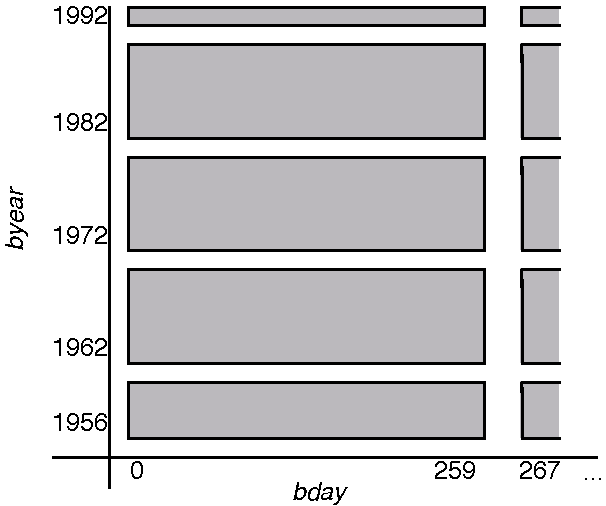
\includegraphics[width=4cm]{figures/bands1.pdf} &
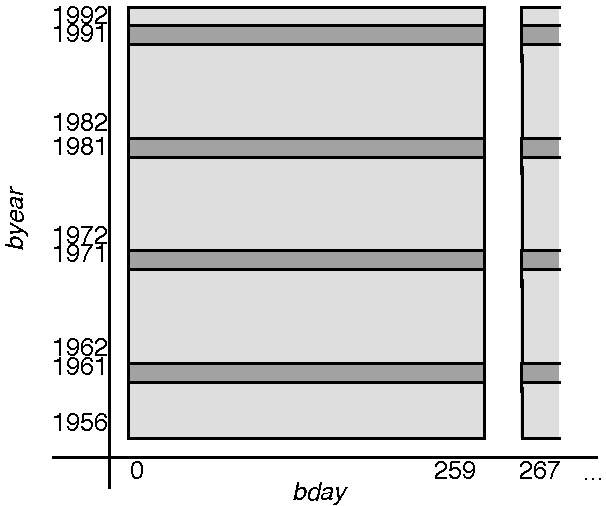
\includegraphics[width=4cm]{figures/bands2.pdf} \\
(a) $\var{output} = \sfalse$ & 
(b) $\var{output} = \strue$ \\
\end{tabular}
\caption{Example 2: most precise revised beliefs}
\label{fig:bands}
\end{figure}

\ifacita 
Running this program reveals nothing about $\var{bday}$, but
does reveal something about $\var{byear}$.  If $\var{output} =
\sfalse$ then the querier knows that $\var{byear} \not\in \{ 1991,
1981, 1971, 1961 \}$, but all other years are equally likely.  We
could represent this new knowledge, combined with the knowledge gained
from the first query, as in Figure~\ref{fig:bands}(a), where
each shaded box is a polyhedron containing equally likely points.  On
the other hand, if $\var{output} = \strue$ then either $\var{byear}
\in \{ 1991, 1981, 1971, 1961 \}$ or the user got lucky.  We represent
the querier's knowledge in this case as in Figure~\ref{fig:bands}(b).
Darker shading indicates higher probability; thus, all years are still
possible, though some are more likely than others.  With the
given threshold of $t_{\var{dy}} = 0.05$, the agent will permit the
query; when $\var{output} = \sfalse$, the likelihood of any point in
the shaded region is $1/11814$; when $\var{output} = \strue$, the
points in the dark bands are the most likely, with probability $
5/13067 $.  Since both outcomes are possible with Bob's $\var{byear} =
1980$, the revised belief will depend on the result of the
probabilistic if statement. 

\else
Running this program reveals
nothing about $\var{bday}$, but does reveal something about
$\var{byear}$.  In particular, if $\var{output} = \sfalse$ then the
querier knows that $\var{byear} \not\in \{ 1991, 1981, 1971, 1961 \}$,
but all other years are equally likely.  We could represent this new
knowledge, combined with the knowledge gained from the first query, as
shown in Figure~\ref{fig:bands}(a), where each shaded box is a
polyhedron containing equally likely points.  On the other hand, if
$\var{output} = \strue$ then either $\var{byear} \in \{ 1991, 1981,
1971, 1961 \}$ or the user got lucky.  We represent the querier's
knowledge in this case as in Figure~\ref{fig:bands}(b).  Darker
shading indicates higher probability; thus, all years are still
possible, though some are much more likely than others.  With the
given threshold of $t_{\var{dy}} = 0.05$, the agent will permit the
query; when $\var{output} = \sfalse$, the likelihood of any point in
the shaded region is $1/11814$; when $\var{output} = \strue$, the
points in the dark bands are the most likely, with probability $
5/13067 $.  Since both outcomes are possible with Bob's $\var{byear} =
1980$, the revised belief will depend on the result of the
probabilistic if statement.
\fi

This example illustrates a potential problem with the simple
representation of probabilistic polyhedra mentioned earlier: when
$\var{output} = \sfalse$ we will jump from using two probabilistic
polyhedra to ten, and when $\var{output} = \strue$ we jump to using
eighteen.  Allowing the number of polyhedra to grow without bound will
result in performance problems. To address this concern, we need a way
to abstract our belief representation to be more concise.
\ifacita
Our technical report~\cite{TR} 
\else
Section~\ref{sec:absinterp} 
\fi
shows how to represent a probabilistic
polyhedron $\pp{}$ as a seven-tuple, $(\getpoly{},\smin{}, \smax{}, \pmin{},
\pmax{}, \mmin{}, \mmax{})$ where $\smin{}$ and $ \smax{}$ are lower
and upper bounds on the number of points with non-zero probability
 in the polyhedron $\getpoly{}$ (called the \textit{support points} of $C$);
the quantities $\pmin{} $ and $ \pmax{} $ are lower and
upper bounds on the probability mass per support point; and $ \mmin{}
$ and $ \mmax{} $ give bounds on the total probability mass. Thus,
polyhedra modeled using the simpler representation $(\getpoly{},m)$
given earlier are equivalent to ones in the more involved
representation with $\mmax{} = \mmin{} = m$, $\pmax{} = \pmin{} = m /
\psize{\getpoly{}}$, and $\smax{} = \smin{} = \psize{\getpoly{}}$.

With this representation, we could choose to collapse the sets of
polyhedron given in Figure~\ref{fig:bands}.  For example, we could
represent Figure~\ref{fig:bands}(a) with two probabilistic polyhedra
$\pp{1}$ and $\pp{2}$ containing polyhedra $\getpoly{1}$ and
$\getpoly{2}$ defined above, respectively, essentially drawing a
box around the two groupings of smaller boxes in the figure.  The
other parameters for $\pp{1}$ would be as follows:
$$
\begin{array}{l}
\pmin{1} = \pmax{1} = 9/135050 \\
\smin{1} = \smax{1} = 8580 \\
\mmin{1} = \mmax{1} = 7722/13505 \\
\end{array}
$$
Notice that $\smin{1} = \smax{2} = 8580 < \psize{\getpoly{1}} = 9620$,
illustrating that the ``bounding box'' of the polyhedron covers more area
than is strictly necessary.  In this representation the probabilities may
not be normalized, which improves both performance and precision.  For this
example, $\pp{2}$ happens to have $\mmin{2} = \mmax{2} = 14553 / 67525 $ so we
can see $\mmax{1} + \mmax{2} = (53163 / 67525) \not= 1$.  

If we consider the representation of
Figure~\ref{fig:bands}(b) in a similar manner, using the same two polyhedra
$\getpoly{1}$ and $\getpoly{2}$, the other parameters for $\getpoly{1}$ are
as follows:
$$
\begin{array}{ll}
\pmin{1} = 1/135050 & \pmax{1} = 10/135050 \\
\smin{1} = 9620 & \smax{1} = 9620 \\
\mmin{1} = 26/185 & \mmax{1} = 26/185 \\
\end{array}
$$
In this case $\smin{1} = \smax{1} = \psize{\getpoly{1}}$, meaning that all
covered points are possible, but $\pmin{1} \not= \pmax{1}$ as some points
are more probable than others (i.e., those in the darker band).

The key property of probabilistic polyhedra, and a main technical
contribution of this paper, is that this abstraction can be used to make
sound security policy decisions.  To accept a query, we must check that, for
all possible outputs, the querier's revised, normalized belief of any of the
possible secrets is below the threshold $t$.  In checking whether the
revised beliefs in our example are acceptable, the agent will try to find
the maximum probability the querier could ascribe to a state, for each
possible output.  In the case $\var{output} = \strue$, the most probable
points are those in the dark bands, which each have probability mass
$10/135050 = \pmax{1}$ (the dark bands in $\pp{2}$ have the same
probability).
% But it is not enough to know
% this value.  We need to know how it compares to the probabilities of
% the other points.  That is, we have to \textit{normalize} the
% distribution before we can find the maximum probability of any point.
To find the maximum normalized probability of these points, we divide by the
minimum possible total mass, as given by the lower bounds in our
abstraction.  In our example, this results in $\pmax{1} / (\mmin{1} +
\mmin{2})$ $=$ $(10/135050) / (26/185 + 49/925) \approx 0.0004 \leq t_{\var{d}} = 0.05$.

As just shown, the bound on minimum total mass is needed in order to soundly
normalize distributions in our abstraction.  The maintenance of such lower
bounds on probability mass is a key component of our abstraction that is
missing from prior work.  Each of the components of a probabilistic
polyhedron play a role in producing the lower bound on total mass.  While
$\smin{1}, \smax{1}, \pmin{1},$ and $\mmax{1}$ do not play a role in making
the final policy decision, their existence allows us to more accurately
update belief during the query evaluation that precedes the final policy
check.  The choice of the number of probabilistic polyhedra to
use impacts both precision and performance, so choosing the right number is
a challenge.  
\ifacita
Section~\ref{sec:impl} shows that our implementation can
often answer these queries in seconds.
\else
For the examples given in this section, our implementation can
often answer queries in a few seconds; details are in Sections
\ref{sec:absinterp}--\ref{sec:impl}.
\fi

\section{Tracking beliefs}
\label{sec:belief}

This section reviews Clarkson et al.'s method of revising a querier's
belief of the possible valuations of secret variables based on the
result of a query involving those
variables~\cite{clarkson09quantifying}.

\begin{figure}[t]
\[
\begin{array}{llcl}
\mathit{Variables} & x & \in & \vars \\ 
\mathit{Integers} & n & \in & \Integer \\
\mathit{Rationals} & q & \in & \Rational \\
\mathit{Arith. ops} & \arithop &::= & + \mid \times \mid - \\
\mathit{Rel. ops} & \relop &::= & \leq \;\mid\; < \;\mid\; = \;\mid\; \neq \;\mid\; \cdots
\\
\mathit{Arith. exps} & \aexp &::= & x \mid n \mid \aop{\aexp_1}{\aexp_2} \\
\mathit{Bool. exps} & \bexp &::= & \bop{\aexp_1}{\aexp_2} \mid \\
% \strue \mid \sfalse \mid \\
& && \bexp_1 \wedge \bexp_2 \mid \bexp_1 \vee \bexp_2 \mid \aneg{\bexp} \\

\mathit{Statements} & \stmt &::= & \sskip \mid \sassign{x}{\aexp} \mid \\
&     && \sif{\bexp}{\stmt_1}{\stmt_2} \mid \\
&     && \spif{q}{\stmt_1}{\stmt_2} \mid \\
&     && \sseq{\stmt_1}{\stmt_2} \mid \swhile{\bexp}{\stmt} % \mid \\
% &     && \suniform{x}{n_1}{n_2} \\
\end{array}
\]
\caption{Core language syntax}
\label{fig:syntax}
\end{figure}

\subsection{Core language}

The programming language we use for queries is given in
Figure~\ref{fig:syntax}.  A computation is defined by a statement
$\stmt$ whose standard semantics can be viewed as a relation between
states: given an input state $\sigma$, running the program will
produce an output state $\sigma'$.  States are maps from variables to
integers:
$$\begin{array}{l}
\sigma, \tau \in \states \defeq \vars \rightarrow \Integer
\end{array}$$
Sometimes we consider states with domains restricted to a
subset of variables $V$, in which case we write $\sigma_V \in \states_V \defeq V
\rightarrow \Integer$.  We may also \emph{project}
states to a set of variables $V$:
\[\project{\sigma}{V} \defeq \lambda x \in \vars_V \lsep \sigma(x)\]

The language is essentially standard. 
\ifacita
We limit the form of expressions to support our abstract
interpretation-based semantics (see the TR version of this paper \cite{TR}).
\else
We limit the form of expressions to support our abstract
interpretation-based semantics (Section~\ref{sec:absinterp}).
\fi
The semantics of the statement form $\spif{q}{\stmt_1}{\stmt_2}$ is
non-deterministic: the result is that of $\stmt_1$ with probability
$q$, and $\stmt_2$ with probability $1 - q$.
% We omit a formal semantics as it is straightforward.

\subsection{Probabilistic semantics for tracking beliefs}
\label{sec:clarkson-semantics}

To enforce a knowledge-based policy, an agent must be able to
estimate what a querier could learn from the output of his query.  To
do this, the agent keeps a distribution $\delta$ that represents
the querier's \emph{belief} of the likely valuations of the user's
secrets.  A distribution is a map from states to positive real
numbers, interpreted as probabilities (in range $[0,1]$).
$$\begin{array}{l}
\delta \in \dists \defeq \states \rightarrow \Real+
\end{array}$$
We sometimes focus our attention on distributions over
states of a fixed set of variables $V$, in which case we write
$\delta_V \in \dists_V$ to mean $\states_V \rightarrow \Real+$.
Projecting distributions onto a set of variables is as
follows:\footnote{The notation $\sum_{x \mid \pi} \rho$ can be read
  \emph{$\rho$ is the sum over all $x$ such that formula $\pi$ is
    satisfied} (where $x$ is bound in $\rho$ and $\pi$).}
\[\project{\delta}{V} \defeq \lambda \sigma_V \in \states_V \lsep \sum_{\sigma' \mid (\project{\sigma'}{V} = \sigma_V)} \delta(\sigma')\]
The \emph{mass} of a distribution, written $ \pmass{\delta} $ is the sum
of the probabilities ascribed to states, $ \sum_{\sigma}
\delta(\sigma) $.  A \emph{normalized distribution} is one such that $
\pmass{\delta} = 1 $.  A normalized distribution can 
be constructed by scaling a distribution according to its
mass:
$$ \normal{\delta} \defeq \frac{1}{\pmass{\delta}} \cdot \delta $$
The \emph{support} of a distribution is the set of states which have
non-zero probability: $\nzset{\delta} \defeq \{\sigma \mid
\delta(\sigma) > 0\}$.

% We take as our basis the denotational semantics for reasoning about belief
% presented by Clarkson et al. \cite{clarkson09quantifying}.


\begin{figure}
%{\small
\centering
\begin{displaymath}
\begin{array}{rcl}
\pevalp{\sskip}{\delta} & = & \delta \\
%
\pevalp{\sassign{x}{\aexp}}{\delta} & = & \delta \bparen{x \ra \aexp} \\
%
\pevalp{\sif{B}{\stmt_1}{\stmt_2}}{\delta} & = &
\pevalp{\stmt_1}{(\dcond{\delta}{B})} + \pevalp{\stmt_2}{(\dcond{\delta}{\neg B})} \\
%
\evalp{\spif{q}{\stmt_1}{\stmt_2}}{\delta} & = & 
\evalp{\stmt_1}{(q \cdot\delta)} + \evalp{\stmt_2}{((1-q) \cdot \delta)} \\
%
\pevalp{\sseq{\stmt_1}{\stmt_2}}{\delta} & = & \pevalp{\stmt_2}{\paren{\evalp{\stmt_1}{\delta}}} \\
\pevalp{\swhile{\bexp}{\stmt}}{} & = & \lfp\left[\lambda
f :\ \dists
\rightarrow \dists \lsep \lambda \delta \lsep \right. \\
& & \left. \quad f\paren{\pevalp{\stmt}{(\dcond{\delta}{B})}} +
       \paren{\dcond{\delta}{\neg B}}\right]
\end{array} 
\end{displaymath} 
where
\begin{displaymath}
\begin{array}{l@{\;\defeq\;}l}
\delta \bparen{x \ra \aexp} & \lambda \sigma \lsep \sum_{\tau \; | \; \tau
  \bparen{x \ra \eeval{\aexp}{\tau}} = \sigma} \delta (\tau) \\
\delta_1 + \delta_2 & \lambda \sigma \lsep \delta_1(\sigma) +
\delta_2(\sigma) \\
\dcond{\delta}{\bexp} & \lambda \sigma \lsep \aif \eeval{\bexp}{\sigma} \athen
\delta(\sigma) \aelse 0 \\
p \cdot \delta & \lambda \sigma \lsep p \cdot \delta(\sigma) \\
\end{array}
\end{displaymath}
%}
\vspace*{-.1in}
\caption{Probabilistic semantics for the core language}
\label{fig-sem-nondet2-core}
\end{figure}

The agent evaluates a query in light of the querier's initial belief using a
probabilistic semantics.  Figure~\ref{fig-sem-nondet2-core} defines a
semantic function $\pevalp{\cdot}{}$ whereby $\pevalp{\stmt}{\delta} =
\delta'$ indicates that, given an input distribution $\delta$, the semantics
of program $\stmt$ is the output distribution $\delta'$.  The semantics is
defined in terms of operations on distributions, including \emph{assignment}
$\delta \bparen{v \ra E}$ (used in the rule for $v := E$),
\emph{conditioning} $\dcond{\delta}{B}$ and \emph{addition} $\delta_1 +
\delta_2$ (used in the rule for $\sifk$), and \emph{scaling} $q \cdot \delta$
where $q$ is a rational (used for $\spifk$).  The semantics is
standard (cf. Clarkson et al.~\cite{clarkson09quantifying}).
\iffull
A brief review is given in Appendix~\ref{appendix:concrete}.
\fi

\subsection{Belief and security}
\label{sec:experiment}

Clarkson et al.~\cite{clarkson09quantifying} describe how a belief
about possible values of a secret, expressed as a probability
distribution, can be revised according to an experiment using the
actual secret.  Such an experiment works as follows.

The values of the set of secret variables $ H $ are given by the hidden
state $\sigma_H$.  The attacker's initial belief as to the possible
values of $\sigma_H$ is represented as a distribution $ \delta_H $.  A
query is a program $ S $ that makes use of variables $ H $ and
possibly other, non-secret variables from a set $L$; the final values
of $L$, after running $S$, are made visible to the attacker.  Let
$\sigma_L$ be an arbitrary initial state of these variables such that
$\dom{\sigma_L} = L$.  Then we take the following steps:

\myparagraph{Step 1} Evaluate $S$ probabilistically using the
querier's belief about the secret to produce an output distribution
$\delta'$, which amounts to the attacker's prediction of the possible output
states.  This is computed as $\delta' = \eval{S}{\delta} $, where
$\delta$, a distribution over variables $ H \uplus L $, is defined
as $ \delta = \delta_H \times \dot{\sigma}_L $.  We make use of
the distribution product operator and point operator.  
That is, given $
\delta_1 $, $ \delta_2 $, which are distributions over states having
disjoint domains, the \emph{distribution product} is
 $$ \delta_1 \times \delta_2 \defeq \lambda(\sigma_1, \sigma_2)
 \lsep \delta_1(\sigma_1) \cdot \delta_2(\sigma_2) $$ where
 $(\sigma_1,\sigma_2)$ is the ``concatenation''
 of the two states, which is itself a state and is
 well-defined because the two states' domains are disjoint.
% \sbmcomment{I wouldn't use the term ``composition'' here.  Maybe ``union''?}
% \sbmcomment{Here is an alternate approach: define projection earlier, and then define product as below.}
%  $$ \delta_1 \times \delta_2 \defeq \lambda \sigma
%  \lsep \delta_1(\project{\sigma}{\dom{\delta_1}}) \cdot \delta_2(\project{\sigma}{\dom{\delta_2}}) $$
% \mwh{This isn't quite right: the domain of $\delta$ is a set of
%   states, but we want to project on a set of variables, i.e., the
%   domain of the domain.  This seems heavier than what's here now.}
And, given a
 state $ \sigma $, the \emph{point distribution} $ \dot{\sigma} $ is a
 distribution in which only $ \sigma $ is possible:
$$ \dot{\sigma} \defeq \lambda \tau \lsep \aif \sigma = \tau \athen 1 \aelse
0 $$ Thus, the initial distribution $\delta$ is the attacker's belief about the
secret variables combined with an arbitrary valuation of the
public variables.

\myparagraph{Step 2} Using the actual
secret $\sigma_H$, evaluate $S$ ``concretely'' to produce an output
state $\hat{\sigma}_L$, in three steps. 
First, we have $\hat{\delta}' = \eval{S}{\hat{\delta}}$, where
$\hat{\delta} = \dot{\sigma}_H \times \dot{\sigma}_L $.  
% Notice here
% that we use the actual secret in constructing the initial
% distribution, rather than the attacker's belief about it. 
Second, we
have $\hat{\sigma} \in \Gamma(\hat{\delta})$ where $\Gamma$ is a sampling
operator that produces a state $\sigma$ from the domain of a
distribution $\delta$ with probability $\delta(\sigma) /
\pmass{\delta}$. Finally, we extract the attacker-visible output of
the sampled state by projecting away the high variables:
$\hat{\sigma}_L = \project{\hat{\sigma}}{L}$.  
% The projection operator
% is defined as $\project{\sigma}{V} \defeq \lambda x \in
% \vars_V \lsep \sigma(x)$.

\myparagraph{Step 3} Revise the attacker's initial belief $\delta_H$
according to the observed output $\hat{\sigma}_L$, yielding a new
belief $\hat{\delta}_H =
\project{\dcond{\delta'}{\hat{\sigma}_L}}{H}$.  Here, $\delta'$ is
\emph{conditioned} on the output $\hat{\sigma}_L$, which yields a new
distribution, and this distribution is then projected to the variables
$H$.  The conditioning is defined as follows:
$$ \dcond{\delta}{\sigma_V} \defeq \lambda \sigma
\lsep \aif \project{\sigma}{V} = \sigma_V \athen \delta (\sigma) \aelse 0 $$
% Second, we have $\hat{\delta}_H =
% \project{\hat{\delta}}{H}$.
%   The latter projection is similar to
% projection on states, given above, but applied to distributions, as
% follows:
% \[
% \project{\delta}{V} \defeq \lambda \sigma_V \in \states_V \lsep \sum_{\sigma' \mid (\project{\sigma'}{V} = \sigma_v)} \delta(\sigma')
% \]
% It allows the querier to
% revise his belief about the secret variables based on the output
% resulting from a query of those secrets.  

\ifacita
\else
Note that this protocol assumes that $S$ always terminates and does not
modify the secret state.  The latter assumption can be eliminated by
essentially making a copy of the state before running the program, while
eliminating the former depends on the observer's ability to detect
nontermination~\cite{clarkson09quantifying}.
\fi
% We say more about
% nontermination as it relates to our approach in the next section.

% A distribution can be projected to a set of variables $ V $:
% $$ \project{\delta}{V}
% = \lambda \sigma_V \lsep \sum_{\sigma : \project{\sigma}{V}
% = \sigma_V} \delta(\sigma) $$
% The projection of a state to $ V $, written $ \project{\sigma}{V} $ as
% above, removes all variables except those of $ V $ from the
% state.

% Given $ \delta $, and a set of
%   states $ S $, we have $\dcond{\delta}{S}$, the revision of $ \delta $,
% The exact behavior is specified as follows:

% $$ \delta | S = \lambda \sigma \lsep \aif \sigma \in S \athen
%   \delta(\sigma) \aelse 0 $$

%   Revision will also be performed based on logical expressions. Having
%   a means of determining whether a logical expression $ B $ is true on a
%   state $ \sigma $, written $ \eeval{B}{\sigma} $, we define revision:

\section{Enforcing knowledge-based policies}
\label{sec:policy}

When presented with a query over a user's data $\sigma_H$, the user's
agent should only answer the query if doing so will not reveal too
much information.  More precisely, given a query $S$, the agent will
return the public output $\sigma_L$ resulting from running $S$ on
$\sigma_H$ if the agent deems that from this output the querier cannot
know the secret state $\sigma_H$ beyond some level of doubt,
identified by a threshold $ t $.  If this threshold could be exceeded,
then the agent declines to run $S$.  We call this security check
\emph{knowledge threshold security}.

\begin{definition}[Knowledge Threshold Security]
\label{def:threshold}
Let $\delta' = \eval{S}{\delta}$, where $\delta$ is the model of the
querier's initial belief.  Then query $S$ is \emph{threshold $ t $
  secure} iff for all $\sigma_L \in \nzset{\project{\delta'}{L}}$ and
all $ \sigma'_H \in \states_H$ we have
$(\project{\drevise{\delta'}{\sigma_L}}{H})(\sigma'_H) \leq t$.
% $(\normal{\project{\paren{\dcond{\delta'}{\sigma_L}}}{H}})(\sigma'_H)
% \leq t$ for some threshold $t$. 
\end{definition}

This definition can be related to the experiment protocol defined in
Section~\ref{sec:experiment}.  First, $\delta'$ in the definition is
the same as $\delta'$ computed in the first step of the protocol.
Step 2 in the protocol produces a concrete output $\hat{\sigma}_L$
based on executing $S$ on the actual secret $\sigma_H$, and Step 3
revises the querier's belief based on this output.
Definition~\ref{def:threshold} generalizes these two steps: instead of
considering a single concrete output based on the actual secret it
considers \emph{all possible} concrete outputs, as given by
$\nzset{\project{\delta'}{L}}$, and ensures that the revised belief in
each case for \emph{all possible} secret states must assign
probability no greater than $t$.

This definition considers a threshold for the whole secret state
$\sigma_H$.  As described in Section~\ref{sec:overview} we can also
enforce thresholds over portions of a secret state.  In particular, a
threshold that applies only to variables $V \subseteq H$ requires that
all $ \sigma'_V \in \states_V$ result in
$(\project{\drevise{\delta'}{\sigma_L}}{V})(\sigma'_V) \leq
t$.

The two ``foralls'' in the definition are critical for ensuring
security.  The reason was shown by the first example in
Section~\ref{sec:overview}: If we used the flawed approach of just
running the experiment protocol and checking if
$\hat{\delta}_H(\sigma_H) > t$ then rejection depends on the value of
the secret state and could reveal information about it.  The more
general policy $\forall \sigma_L \in \nzset{\project{\delta'}{L}}.\,
(\project{\drevise{\delta'}{\sigma_L}}{H})(\sigma_H) \leq t $, would
sidestep the problem in the example, but this policy could still
reveal information because it too depends on the actual secret
$\sigma_H$.
% (An example illustrating the problem in this case is given in 
% Appendix~\ref{appendix:flawed}.)

Definition~\ref{def:threshold} avoids any inadvertent information
leakage because rejection is not based on the actual secret: if there
exists \emph{any} secret such that a possible output would reveal too
much, the query is rejected. Definition~\ref{def:threshold} is
equivalent to a worst-case \emph{conditional vulnerability} (upper)
bound or alternatively a worst-case \emph{conditional min-entropy}
(lower) bound. Min-entropy measures the expected likelihood of an
adversary guessing the secret value \cite{smith09foundations}; the
stronger worst-case used in our definition does away with expectation
and bounds this likelihood regardless of what the secret is. Such
worst-case measures were considered in \cite{koepfbasin07} as a means
of providing a stronger security guarantee. In our case, however, the
extra strength is a side-effect of our need for a simulatable
policy. See Section~\ref{sec:related} for further details.

% In fact, the use
% of a simple maximum probability threshold $ t $ corresponds to a
% minimum relative entropy $ - \lg t $ between the true belief and the
% revised belief ~\cite{clarkson09quantifying}.

% To make belief revision cost effective, we restrict queries to boolean
% results.  By fixing the output space of a query to two values, the
% security policy can be implemented by a single abstract interpretation
% of the query according to the attacker's modeled belief followed by
% two revision operations (which employ polyhedral intersections).  For
% many domains, boolean queries are perfectly acceptable (e.g., should a
% particular ad be shown to a given user), and larger output spaces can
% be handled by multiple queries (e.g., using a directed search).

% I'm convinced by Peter's examples of min / max total mass being
% useful.  It will be interesting to see what types of calculations end
% up being most prevalent in our examples.  The interplay between total
% mass and the per-point mass function is interesting and seems like the
% sort of thing that mathematicians may have considered before.  I did
% some minor digging and Simplexes seem related:

% http://en.wikipedia.org/wiki/Simplex
% (also see http://en.wikipedia.org/wiki/Categorical_distribution)

% As a bonus, n-dimensional simplexes correspond directly to
% n-dimensional convex polyhedra.  One big difference between our
% distribution sets and simplexes is that we have bounds on the number
% of 0-valued points.

% Anyway, something to think about after we get this paper written.  I
% suspect there is a large space of possible abstractions for these
% distributions and it will be interesting to compare them (once we
% discover them :-)

\section{Belief revision via abstract interpretation}
\label{sec:absinterp}

\setlength{\arraycolsep}{0.1cm}
\newcommand{\ajoin}[0]{\bigsqcup}

% We could implement the belief semantics described in the previous
% section more-or-less directly, e.g., using an existing probabilistic
% language (such as IBAL~\cite{pfeffer07ibal} or Probabilistic
% Scheme~\cite{radul07probscheme}).  However, existing approaches use
% sampling to perform belief revisions, and for the examples of the sort
% given in Section~\ref{sec:examples}, the input space is too large for
% sampling to compute sound answers efficiently.  Therefore, we have
% developed a probabilistic semantics using abstract
% interpretation.

Consider how we might implement belief tracking and revision to
enforce the threshold security property given in
Definition~\ref{def:threshold}.  A natural choice would be to evaluate
queries using a probabilistic programming language with support for
conditioning, of which there are many \cite{pfeffer07ibal,
  radul07probscheme, park08sampling, goodman08church,
  kiselyov09embedded, claret12bayesian, milch05blog,
  borgstrom11measure}.  Such languages are largely
ineffective for use in ensuring security guarantees. Approximate
inference in these languages cannot ensure security guarantees, while
exact inference, due to its lack of abstraction facilities, can be too
inefficient when the state space is large.

%As more inputs are enumerated, a more complete view of the
%output distribution emerges.  Unfortunately, to get an accurate
%estimate of the revised distribution following an output observation,
%one must enumerate the entire input space, which could be quite large.
%If insufficient coverage is achieved, then the threshold check in
%Definition~\ref{def:threshold} could either be unsound or excessively
%conservative, depending in which direction an implementation errs.

We have developed a new means to perform probabilistic computation
based on abstract interpretation.  In this approach, execution time
depends on the complexity of the query rather than the size of the
input space.  In the next two sections, we present two abstract
domains.  This section presents the first, denoted $\ppolys$, where an
abstract element is a single \emph{probabilistic polyhedron}, which is
a convex polyhedron~\cite{CousotHalbwachs78-POPL} with information
about the probabilities of its points. 

Because using a single polyhedron will accumulate imprecision after
multiple queries, in our implementation we actually use a different
domain, denoted $ \ppowers $, for which an abstract element consists
of a set of at most $n$ probabilistic polyhedra (whose construction is
inspired by powersets of polyhedra
\cite{bagnara06powerset,Popeea06inferringdisjunctive}).  This domain,
described in the next section, allows us to retain precision at the
cost of increased execution time.  By adjusting $n$, the user can
trade off efficiency and precision. An important element of our
approach is the ability to soundly evaluate the knowledge-threshold
policies, even under approximate inference.

\subsection{Polyhedra} \label{sec:polyhedra}

We first review \emph{convex polyhedra}, a common technique for representing sets of program states.  We use the meta-variables $\ineq, \ineq_1, \ineq_2$, etc. to denote linear inequalities.  We write $\fv\ineq$ to be the set of variables occurring in
$\ineq$; we also extend this to sets, writing $\fv{\{\ineq_1,\ldots,\ineq_n\}}$ for $\fv{\ineq_1} \cup \ldots \cup \fv{\ineq_n}$.

\begin{definition}
  A \emph{convex polyhedron} $\poly = (\cons, V)$ is a set of linear inequalities
  $\cons = \{\ineq_1,\ldots,\ineq_m\}$, interpreted conjunctively,
  over dimensions $ V $.  We write
  $\cp$ for the set of all convex polyhedra.   A polyhedron $\poly$
  represents a set of states, denoted $\pconc{\poly}$, as follows, where $\sigma \models \ineq$ indicates that the state $\sigma$ satisfies the inequality $\ineq$.
\[\pconc{\paren{\cons,V}} \defeq \{\sigma \given \fv{\sigma} =
V,\; \forall \ineq \in \cons.\ \sigma \models \ineq\}\]

Naturally we require that $\fv{\{\ineq_1,\ldots,\ineq_n\}} \subseteq V
$. We write $ \fv{\paren{\cons, V}} $ to denote the set of variables $
V $ of a polyhedron.

\end{definition}

% Figure \ref{fig:polyhedra} gives an example of a
% polyhedron $\poly$ and the set of states $\pconc{\poly}$.
Given a state $\sigma$ and an ordering on the variables in $\fv{\sigma}$, we can view $\sigma$ as a point in
an $N$-dimensional space, where $N = \setsize{\fv{\sigma}}$.  The set $\pconc{\poly}$ can then be viewed as the integer-valued lattice points in an $N$-dimensional polyhedron.
Due to this correspondence, we use the words \textit{point} and
\textit{state} interchangeably.  We will sometimes write linear equalities $x = f(\vec{y})$ as an abbreviation for the pair of inequalities $x \leq f(\vec{y})$ and $x \geq f(\vec{y})$.
% \todo{TODO: draw this picture.}

\newcommand{\myitem}{~\\ \noindent $\bullet$ }
Let $ \poly = (\cons, V) $. Convex polyhedra support the following
operations.
\begin{itemize}
%   We
% write $\setsize{S}$ to represent the cardinality of the set $S$.
\item Polyhedron size, or $ \psize{\poly} $, is the number of
   integer points in the polyhedron, i.e., $\setsize{\pconc{\poly}}$.
   We will always consider bounded polyhedra when determining their
   size, ensuring that $\psize{\poly}$ is finite.
\item (Logical) expression evaluation, $\abseeval{\bexp}{\poly}$ returns a
   convex polyhedron containing at least the points in $\poly$ that satisfy
$\bexp$. Note that $ B $ may or may not have disjuncts.
\item Expression count, $\absecount{\bexp}{\poly}$ returns an upper bound
 on the number of integer points in $\poly$ that satisfy $\bexp$. Note
 that this may be more precise than $\psize{\abseeval{\bexp}{\poly}}$
 if $ B $ has disjuncts.
% \sbmcomment{Because these are abstract operations (and may be approximate).
% $\absecount{\bexp}{\poly} \leq \psize{\abseeval{\bexp}{\poly}}$ but they may
% not be equal (and will not be for polyhedra).  Image the condition $\neg(x = 0)$.
% If $\poly$ is $-5 \leq x \leq 5$ then $\abseeval{\bexp}{\poly}$ is $-5 \leq x \leq 5$,
% which has 11 points, while $\absecount{\bexp}{\poly}$ could return $10$.
% Our implementation of $\absecount{\bexp}{\poly}$ proceeds by introducing some
% disjunction (thus retaining more precision) before doing the counting.  So it would count
% the points in the two polyhedra given by $-5 \leq x \leq -1$ and $1 \leq x \leq 5$.
% (These disjuncts can then either be thrown away or kept, depending on whether we are
% in the single polyhedron domain or the powerset domain.)
% While we implement a rather roundabout way of computing points consistent with $\bexp$
% (introduce disjunctions, take intersections, count),
% it's possible that a more direct method could be devised.  In any case, given the fact
% that considering this operation separately can improve precision, it seemed worth keeping
% it separate.  It also corresponds nicely with $\abseeval{\bexp}{\poly}$ (which is
% more precise than its ``naive'' implementation as $\poly \pmeet \alpha(\bexp)$, where
% $\alpha$ is the abstraction function returning the smallest convex polyhedron containing $\bexp$).
% }
 \item Meet, $ \pa \pmeet \pb $ is the convex
 polyhedron containing exactly the set of points in the intersection of
 $\pconc{\pa}, \pconc{\pb}$.
\item Join, $\pa \pjoin \pb$ is the smallest convex
 polyhedron containing both $\gamma(\pa)$ and $\gamma(\pb)$.
\item Comparison, $\pa \pord \pb$ is a partial order whereby $\pa \pord \pb$ if and only if $\pconc{\pa} \subseteq \pconc{\pb}$.
\item Affine transform, $\poly \bparen{x \ra \aexp}$, where $x
  \in \fv{\poly} $, computes an affine transformation of $ \poly $.  This scales
  the dimension corresponding to $x$ by the coefficient of $x$ in
  $\aexp$ and shifts the polyhedron.  For example, $\paren{\{x \leq y, y =
  2z\}, V} \bparen{y \ra z + y}$ evaluates to $\paren{\{x \leq y - z, y - z =
  2z\}, V}$.
\item Forget, $\forget{x}{\poly}$, projects away $x$.  That is,
  $\forget{x}{\poly} = \pi_{\fv{\poly}-\{x\}}(\poly)$, where
  $\pi_V(\poly)$ is a polyhedron $\poly'$ such that $\pconc{\poly'} =
  \{ \sigma \given \tau \in \pconc{\poly} \wedge \sigma =
  \project{\tau}{V} \}$.  So $\poly' = \forget{x}{\poly}$ implies
  $x \not\in fv(\poly')$. The projection of $ \getpoly{} $ to
  variables $ V $, written $ \project{\getpoly{}}{V}$ is defined as
  the forgetting of all the dimensions of $ \getpoly{} $ other than $
  V $.
%\item{} Add dimensions, $ \newdim{V'}{\poly} $ is the polyhedron with
%  additional dimensions $ V' $ that are disjoint from $ \fv{\poly} $. Thus $
%  \fv{\newdim{V'}{\poly}} = \fv{\poly} \cup V' $ with the dimensions $ V'
%  $ unconstrained. If $ V' = \set{x_1, \cdots, x_m} $ then $
%  \pconc{\newdim{V'}{C}} = \set{\sigma \cup \set{x_i = n_i}_{i=1}^{m}
%    \given \sigma \in \pconc{C}, n_i \in \Integer} $.  We write $
%  \sigma \cup \set{x = n} $ to denote a state $ \sigma $ with an
%  additional assignment of $ x $ to value $ n $. 
\item{} Linear partition $\partn{\getpoly{A}}{\getpoly{B}}$  
  of two (possibly overlapping) polyhedra $ \getpoly{A} $, $
  \getpoly{B} $ is a set of equivalent disjoint polyhedra $
  \set{\getpoly{i}}_{i=1}^{n} $. That is, $ \cup_i \pconc{\getpoly{i}}
  = \pconc{\getpoly{A}} \cup \pconc{\getpoly{B}} $ and $
  \pconc{\getpoly{i}} \cap \pconc{\getpoly{j}} = \emptyset $ for $ i
  \neq j $.  When $\getpoly{A}$ and $\getpoly{B}$ do not overlap then
  $\partn{\getpoly{A}}{\getpoly{B}} = \set{\getpoly{A},\getpoly{B}}$.
\end{itemize}

We write $\isempty{\poly}$ \emph{iff} $\pconc{\poly} = \emptyset$.

\subsection{Probabilistic Polyhedra}

We take this standard representation of sets of program states and
extend it to a representation for sets of distributions over program
states.  We define \emph{probabilistic polyhedra}, the core element of
our abstract domain, as follows.

\begin{definition} \label{def:ppoly}
A \emph{probabilistic polyhedron} $\pp{}$ is a tuple
$(\getpoly{},\smin{},$ $\smax{}, \pmin{},$ $\pmax{}, \mmin{},$ $\mmax{})$.  
We write $\ppolys$ for the set of probabilistic polyhedra.  The
quantities $\smin{}$ and $ \smax{}$ are lower and upper bounds on 
the number of support points in the polyhedron $\getpoly{}$.  The quantities
$\pmin{} $ and $ \pmax{} $ are lower and upper bounds on the
probability mass \emph{per support point}.  The $ \mmin{} $ and $
\mmax{} $ components give bounds on the total probability mass.  
Thus $\pp{}$ represents the \emph{set} of distributions
$\ppconc{\pp{}}$ defined below. 
\[
\ppconc{\pp{}} \defeq
\begin{aligned}[t]
\{\delta \given {} & \nzset{\delta} \subseteq \pconc{\getpoly{}} \wedge {} \\
  & \smin{} \leq \setsize{\nzset{\delta}} \leq \smax{} \wedge {} \\
  & \mmin{} \leq \pmass{\delta} \leq \mmax{} \wedge \\
  & \forall \sigma \in \nzset{\delta}.\ \pmin{} \leq \delta(\sigma) \leq \pmax{}\}
\end{aligned}
\]

We will write $ \fv{\pp{}} \defeq \fv{\poly} $ to denote the set of variables
used in the probabilistic polyhedron. 

\end{definition}
% Recall that $\pmass{\delta}$ gives the mass of distribution $\delta$,
% which is the sum of the probabilities ascribed to states by $\delta$. 
Note the set $\ppconc{\pp{}}$ is a singleton exactly when $\smin{} =
\smax{} = \psize{\getpoly{}}$ and $\pmin{} = \pmax{}$, and $\mmin{} =
\mmax{}$.  In such a case $\ppconc{\pp{}}$ contains only the uniform
distribution where each state in $\pconc{\getpoly{}}$ has probability
$\pmin{}$. In general, however, the concretization of a probabilistic
polyhedron will have an infinite number of distributions. For example,
the pair of probabilistic polyhedra in \sref{sec:overview},
Equation~\ref{eq-nonuniform} admits an infinite set of distributions,
with per-point probabilities varied somewhere in the range $ \pmin{1}
$ and $ \pmax{1} $. The representation of the non-uniform distribution
in that example is thus approximate, but the security policy can still
be checked via the $ \pmax{1} $ (and $ \mmax{2} $) properties of the
probabilistic polyhedron.

Distributions represented by a probabilistic polyhedron
are not necessarily normalized (as was true in
Section~\ref{sec:clarkson-semantics}).  In general, there is a
relationship between $\pmin{}, \smin{}, $ and $\mmin{}$, in that
$\mmin{} \geq \pmin{} \cdot \smin{}$ (and $\mmax{} \leq \pmax{} \cdot
\smax{}$), and the combination of the three can yield more information
than any two in isolation.

Our convention will be to use $\getpoly{1}$, $\smin{1}$, $\smax{1}$,
etc. for the components associated with probabilistic polyhedron
$\pp{1}$ and to use subscripts to name different probabilistic
polyhedra.

\myparagraph{Ordering}
Distributions are ordered point-wise~\cite{clarkson09quantifying}.
That is, $\delta_1 \leq \delta_2$ if and only if $\forall
\sigma.\ \delta_1(\sigma) \leq \delta_2(\sigma)$.  For
our abstract domain, we say that $\pp{1} \ppord \pp{2}$ if and only if
$\forall \delta_1 \in \ppconc{\pp{1}}.\ \exists \delta_2 \in
\ppconc{\pp{2}}.\ \delta_1 \leq \delta_2$.  Testing $\pp{1} \ppord
\pp{2}$ mechanically is non-trivial, but is unnecessary in our
semantics.  Rather, we need to test whether a distribution
represents only the zero distribution $\distzero \defeq \lambda
\sigma. 0$ in order to see that a fixed point for evaluating
$\abspevalp{\swhile{\bexp}{\stmt}}{\pp{}}$ has been reached.
Intuitively, no further iterations of the loop need to be considered
once the probability mass flowing into the $n^\text{th}$ iteration is
zero. This condition can be detected as follows:
% \vspace*{-0.9em}
% \begin{small}
\[
\begin{array}{l}
\iszero{\pp{}} \defeq \\
\qquad \paren{\smin{} = \smax{} = 0 \wedge \mmin{} = 0 \leq \mmax{}} \\
\quad \vee\; \paren{\mmin{} = \mmax{} = 0 \wedge \smin{} = 0 \leq \smax{}} \\
\quad \vee\; \paren{\isempty{\poly} \wedge \smin{} = 0 \leq \smax{} \wedge
\mmin{} = 0 \leq \mmax{}} \\
\quad \vee\; \paren{\pmin{} = \pmax{} = 0 \wedge \smin{} = 0 \leq \smax{} \wedge
\mmin{} = 0 \leq \mmax{}} \\
\end{array}
\]
% \end{small}
If $ \iszero{\pp{}} $ holds, it is the case that $ \ppconc{\pp{}} =
\set{\distzero} $.  This definition distinguishes $\ppconc{\pp{}} =
\emptyset $ (if $ \pp{} $ has inconsistent constraints) from 
$\ppconc{\pp{}} = \set{\distzero} $.  Note that having a more
conservative definition of $\iszero{\pp{}}$ (which holds for fewer
probabilistic polyhedra $\pp{}$) would simply mean our analysis would
terminate less often than it could, with no effect on
security.
%If $ \iszero{\pp{}} $ holds, it is the case that $ \ppconc{\pp{}} =
%\set{\distzero} $.  This definition has been carefully crafted to
%avoid treating a polyhedron with inconsistent constraints (which could
%arise when abstractly interpreting dead code) as being equivalent to
%$\set{\distzero}$; i.e., we must distinguish when $\ppconc{\pp{}} =
%\emptyset $ (arising from inconsistent constraints) from when
%$\ppconc{\pp{}} = \set{\distzero} $.  Note that having a more
%conservative definition of $\iszero{\pp{}}$ (which holds for fewer
%probabilistic polyhedra $\pp{}$) would simply mean our analysis would
%terminate less often than it could, with no effect on
%security. 

Following standard abstract interpretation terminology, we will refer
to $\powerset{\dists}$ (sets of distributions) as the \textit{concrete
  domain}, $\ppolys$ as the \textit{abstract domain}, and $\ppconcfun
: \ppolys \rightarrow \powerset{\dists}$ as the \textit{concretization
  function} for $\ppolys$.


\subsection{Abstract Semantics for $\ppolys$}

To support execution in the abstract domain just defined, we need
to provide abstract implementations of the basic operations of assignment,
conditioning, addition, and scaling used in the concrete semantics given in
Figure \ref{fig-sem-nondet2-core}.  We will overload notation and use the
same syntax for the abstract operators as we did for the concrete operators.

As we present each operation, we will also state the associated
soundness theorem which shows that the abstract operation is an
over-approximation of the concrete operation. Proofs are given in a
separate technical report~\cite{TR}.

The abstract program semantics is then exactly the semantics from
Figure \ref{fig-sem-nondet2-core}, but making use of the abstract
operations defined here, rather than the operations on distributions
defined in Section \ref{sec:clarkson-semantics}.  We will write
$\abspevalp{S}{\pp{}}$ to denote the result of executing $S$ using the
abstract semantics.  The main soundness theorem we obtain is the
following.
\begin{theorem}
\label{thm:pp:soundness}
For all $\pp{}, \delta$, if $ \delta \in \ppconc{\pp{}} $ and
$ \abspevalp{S}{\pp{}} $ terminates, then $ \pevalp{S}{\delta} $ terminates and $
\pevalp{S}{\delta} \in \ppconc{\abspevalp{S}{\pp{}}} $.
\end{theorem}

When we say $ \pevalp{S}{\delta} $ terminates (or $
\abspevalp{S}{\pp{}} $ terminates) we mean that only a finite number
of loop iterations are required to interpret the statement on a
particular distribution (or probabilistic polyhedron). In the concrete
semantics, termination can be checked by iterating until the mass of $
\dcond{\delta}{B} $ (where $ B $ is a guard) becomes zero. (Note that
$ \pevalp{S}{\delta} $ is always defined, even for infinite loops, as
the least fixed-point is always defined, but we need to distinguish
terminating from non-terminating loops for security reasons, as per
the comment at the end of Section~\ref{sec:experiment}.) 
To check termination in the
abstract semantics, we check that upper bound on the mass of $
\absdcond{\pp{}}{B} $ becomes zero. 
%
In a standard abstract domain, termination of the
fixed point computation for loops is often ensured by use of a widening
operator.  This allows abstract fixed points to be computed in fewer
iterations and also permits analysis of loops that may not terminate.
In our setting, however, non-termination may reveal information about secret
values.  As such, we would like to reject queries that may be non-terminating.

We enforce this by not introducing a widening
operator~\cite{CousotHalbwachs78-POPL,cortesi08widening}.  Our abstract
interpretation then has the property that it will not terminate if a
loop in the query may be non-terminating (and, since it is an
over-approximate analysis, it may also fail to terminate even for some
terminating computations).  We then reject all queries for which our
analysis fails to terminate in some predefined amount of time.  Loops
do not play a major role in any of our examples, and so this approach
has proved sufficient so far.  We leave for future work the
development of a widening operator that soundly accounts for
non-termination behavior.

% The precise definitions of termination can be found in
% Appendix~\ref{appendix:proof1}.

The proof for \tref{thm:pp:soundness} is a structural induction on $ S
$; the meat of the proof is in the soundness of the various abstract
operations. The following sections present these abstract
operations and their soundness relative to the concrete
operations. The basic structure of all the arguments is the same: the
abstract operation over-approximates the concrete one.

\subsubsection{Forget} \label{sec:forget}

We first describe the abstract forget operator $\forget{y}{\pp{1}}$,
which is used in implementing assignment. Our abstract implementation
of the operation must be sound relative to the concrete one,
specifically, if $\delta \in \ppconc{\pp{}}$ then $\forget{y}{\delta}
\in \ppconc{\forget{y}{\pp{}}}$.

The concrete forget operation projects away a single dimension:
\begin{align*}
\forget{x}{\delta}
  & \defeq \project{\delta}{\paren{\fv{\delta} - \set{x}}} \\
  & = \lambda \sigma_V \in \states_V \lsep \sum_{\tau \given
  \project{\tau}{V} = \sigma_V} \delta(\tau) & \text{where $ V
= \fv{\delta} - \set{x} $}
\end{align*}
When we forget variable $y$, we collapse any states that are
equivalent up to the value of $y$ into a single state.

To do this soundly, we must find an upper bound
$\maxh{y}$ and a lower bound $\minh{y}$ on the number of integer
points in $ \getpoly{1}$ that share the value of the remaining
dimensions (this may be visualized of as the min and max height of
$\getpoly{1}$ in the $y$ dimension). More precisely, if $ V =
\fv{\getpoly{1}} - \set{y} $, then for every $ \sigma_V \in
\pconc{\project{\getpoly{1}}{V}} $ we have $ \minh{y} \leq
\setsize{\set{\sigma \in \pconc{\getpoly{1}}: \project{\sigma}{V} =
    \sigma_V}} \leq \maxh{y} $.  Once these values are obtained, we
have that $\forget{y}{\pp{1}} \defeq \pp{2}$ where the following hold
of $\pp{2}$.
\[
\begin{array}{lcl@{\hspace{0.4cm}}|@{\hspace{0.4cm}}lcl}
\poly_2 &=& \multicolumn{4}{l}{\forget{y}{\poly_1}} \bigstrut[b] \\
\pmin{2} &=& \multicolumn{4}{l}{\pmin{1} \cdot \maxparen{\minh{y}-(\psize{\poly_1} - \smin{1}),\ 1}} \bigstrut \\
\pmax{2} &=& \multicolumn{4}{l}{\pmax{1} \cdot \minparen{\maxh{y},\ \smax{1}}} \bigstrut \\
\smin{2} &=& \lceil{\smin{1} / \maxh{y}}\rceil &
  \mmin{2} &=& \mmin{1} \bigstrut \\
\smax{2} &=& \minparen{\psize{\forget{y}{\poly_1}},\ \smax{1}} &
  \mmax{2} &=& \mmax{1} \bigstrut[t]
\end{array}
\]

The new values for the under and over-approximations of the various
parameters are derived by reasoning about the situations
in which these quantities could be the smallest or the greatest,
respectively, over all possible $ \delta_2 \in \ppconc{\pp{2}} $ where
$ \delta_2 = \forget{y}{\delta_1} $, $ \delta_1 \in \ppconc{\pp{1}}
$. We summarize the reasoning behind the calculations below:
\begin{itemize}
\item{} $ \pmin{2} $: The minimum probability per support point is
  derived by considering a point of $ \pp{2} $ that had the least
  amount of mass of $ \pp{1} $ mapped to it. Let us call this point $
  \sigma_V $ and the set of points mapped to it $ S = \set{\sigma
      \in \pconc{\getpoly{1}} \given \project{\sigma}{V} = \sigma_V}$.
    $ S $ could have as little as $ \minh{y} $ points, as
    per definition of $ \minh{y} $ and not all of these points must be
    mass-carrying. There are at least $ \smin{1} $ mass-carrying
    points in $ \getpoly{1} $. If we assume that as many as possible
    of the mass carrying points in the region $ \getpoly{1} $ are
    outside of $ S $, it must be that $ S $ still contains at least
    $\minh{y}-(\psize{\poly_1} - \smin{1})$ mass carrying-points, each
    having probability at least $ \pmin{1} $.
\item{} $ \pmax{2} $: The maximum number of points of $ \pp{1} $ that
  get mapped to a single point in $ \pp{2} $ cannot exceed $ \smax{1}
  $, the number of support points in $ \pp{1} $. Likewise it cannot
  exceed $ \maxh{y} $ as per definition of $ \maxh{y} $.
\item{} $ \smin{2} $: There cannot be more than $ \maxh{y} $ support
  points of $ \pp{1} $ that map to a single point in $ \pp{2} $ and
  there are at least $ \smin{1} $ support points in $ \pp{1} $. If we
  assume that every single support point of $ \pp{2} $ had the maximum
  number of points mapped to it, there would still be $ \ceil{\smin{1}
    / \maxh{y}} $ distinct support points in $ \pp{2} $.
\item{} $ \smax{2} $: The maximum number of support points cannot
  exceed the size of the region defining $ \pp{2} $. It also cannot
  exceed the number of support points of $ \pp{1} $, even if we
  assumed there was a one-to-one mapping between the support points of
  $ \pp{1} $ and support points of $ \pp{2} $.
\end{itemize}


\begin{figure}
\begin{center}
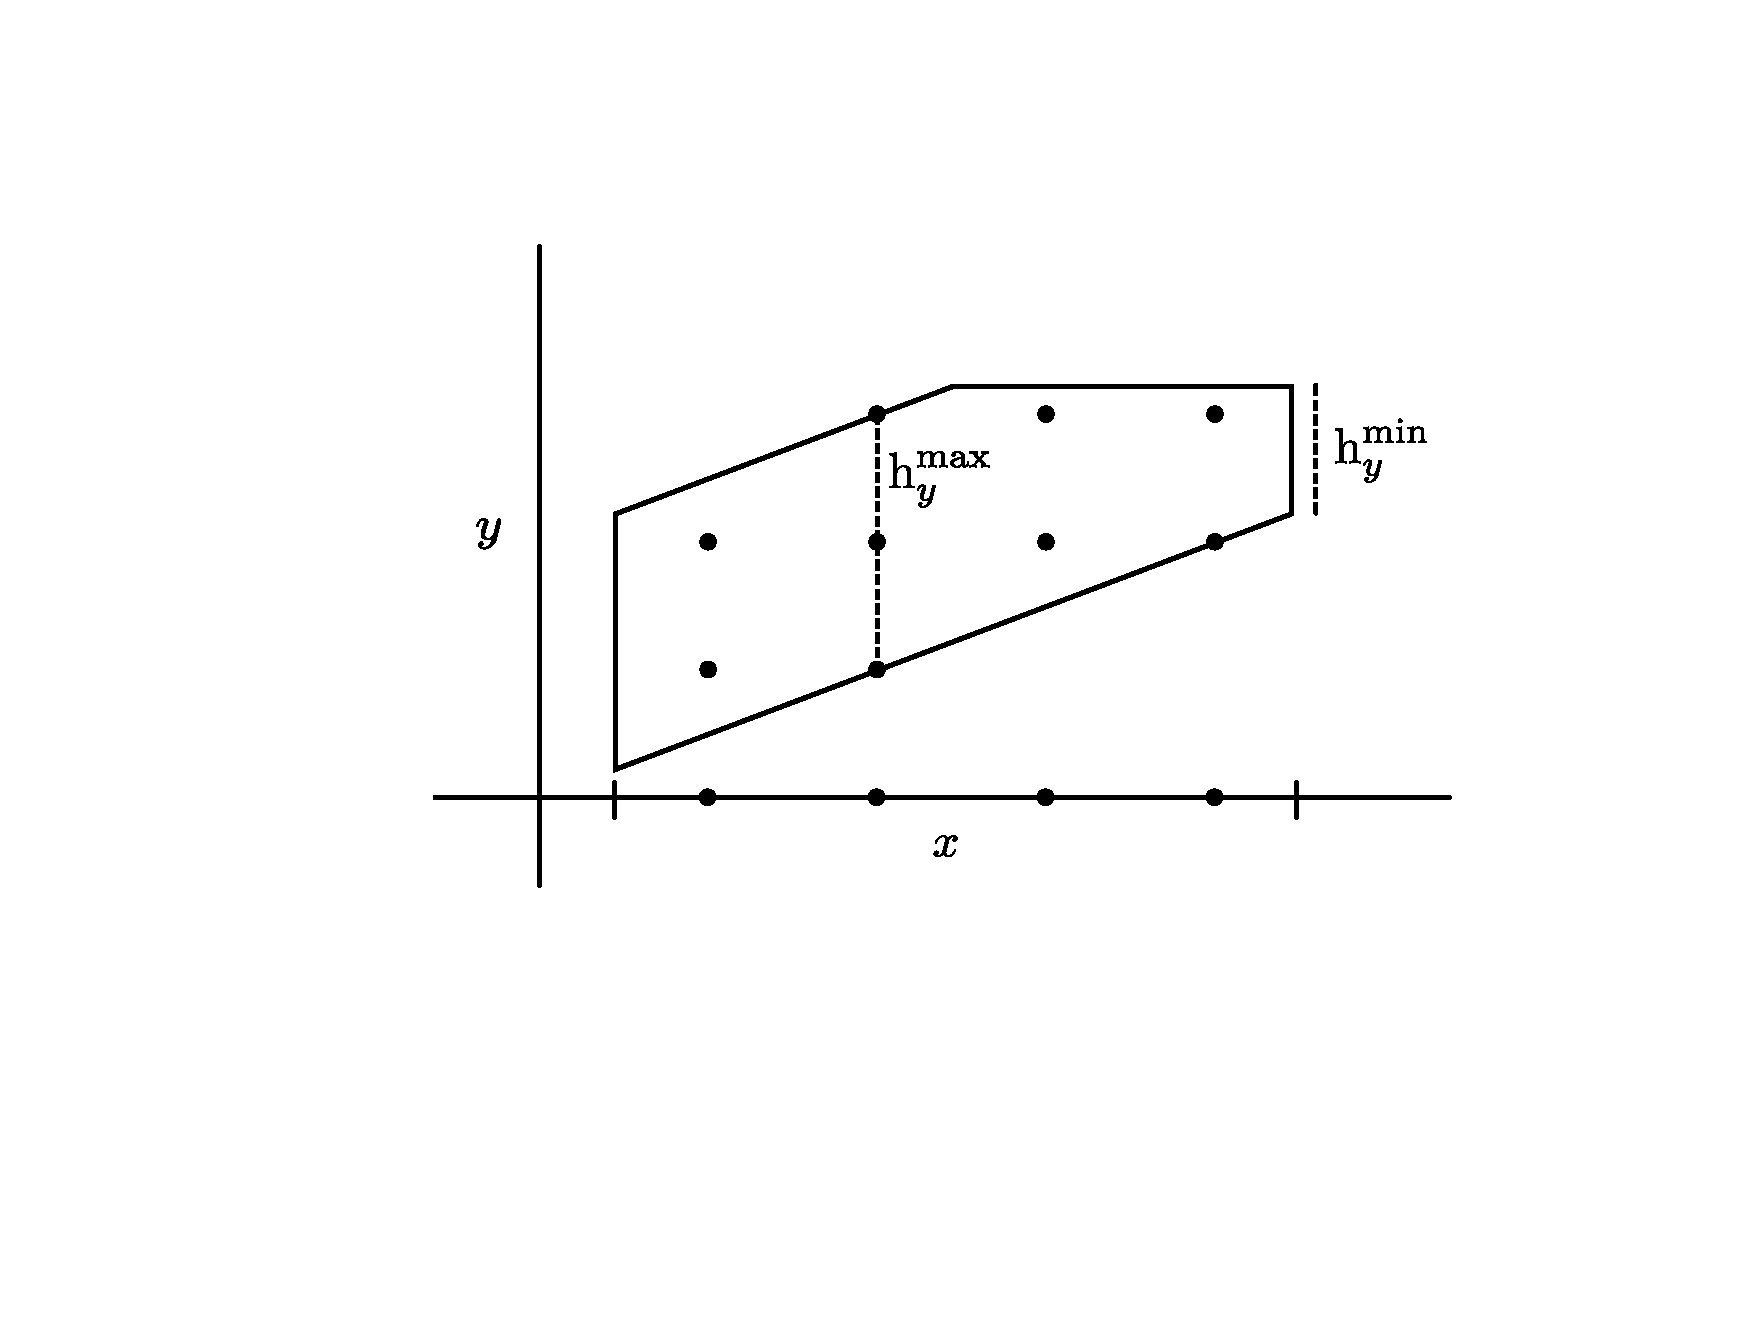
\includegraphics[width=6.5cm]{figures/forget.pdf} % !!! commented out slow figure
\end{center}
\caption{\label{fig:forget} Example of a forget operation in the abstract domain $\ppolys$.  In this case, $\minh{y} = 1$ and $\maxh{y} = 3$.  Note that $\maxh{y}$ is precise while $\minh{y}$ is an under-approximation.  If $\smin{1} = \smax{1} = 9$ then we have $\smin{2} = 3$, $\smax{2} = 4$, $\pmin{2} = \pmin{1} \cdot 1$, $\pmax{2} = \pmax{2} \cdot 4$.}
\end{figure}

Figure \ref{fig:forget} gives an example of a forget operation and
illustrates the quantities $\maxh{y}$ and $\minh{y}$.  If $ \poly_1 =
(\cons_1, V_1) $, the upper bound $\maxh{y}$ can be found by maximizing $y - y'$ subject to the
constraints $\cons_1 \cup \cons_1[y' / y]$, where $y'$ is a fresh variable and $\cons_1[y'/y]$ represents the set of
constraints obtained by substituting $y'$ for $y$ in $\cons_1$.  As our
points are integer-valued, this is an integer linear programming
problem (and can be solved by ILP solvers). A less precise upper bound
can be found by simply taking the extent of the polyhedron $\getpoly{1}$ along $y$,
which is given by $\psize{\pi_y(\getpoly{1})}$.

For the lower bound, it is always sound to use $\minh{y} = 1$. A more
precise estimate can be obtained by treating the convex polyhedron as
a subset of $ \Real^n $ and finding the vertex with minimal height
along dimension $y$. Call this distance $u$. An example of this
quantity is labeled $ \minh{y} $ in \fref{fig:forget}. Since the shape
is convex, all other points will have $y$ height greater than or equal
to $u$. We then find the smallest number of integer points that can be
covered by a line segment of length $u$. This is given by $\lceil u
\rceil - 1$.  The final under-approximation is then taken to be the
larger of $ 1 $ and $ \lceil u \rceil -1 $. As this method requires us
to inspect every vertex of the convex polyhedron and to compute the
$y$ height of the polyhedron at that vertex, we can also look for the
one upon which the polyhedron has the greatest height, providing us
with the estimate for $ \maxh{y} $.

\begin{lemma}
\label{lem:pp:forget}
If $\delta \in \ppconc{\pp{}}$ then $\forget{y}{\delta} \in
\ppconc{\forget{y}{\pp{}}}$.
\end{lemma}
\noindent
We can define an abstract version of projection using forget:
\begin{definition}
Let $\forget{\{x_1,x_2,\ldots,x_n\}}{\pp{}} =
\forget{\{x_2,\ldots,x_n\}}{\forget{x_1}{\pp{}}}$.  Then
$\project{\pp{}}{V'} = \forget{(\fv{\pp{}} - V')}{\pp{}}$. 
\end{definition}
That is, in order to project onto the set of variables $V'$, we forget
all variables not in $V'$.

\subsubsection{Assignment}
The concrete assignment operation is defined so that the probability
of a state $ \sigma $ is the accumulated probability mass of all
states $ \tau $ that lead to $ \sigma $ via the assignment:
$$ \delta \bparen{x \ra \aexp} \defeq \lambda \sigma \lsep \sum_{\tau \given \tau
  \bparen{x \ra \eeval{\aexp}{\tau}} = \sigma} \delta (\tau) $$

The abstract implementation of this operation strongly depends on the
invertibility of the assignment. Intuitively, the set $ \set{\tau
  \given \tau \bparen{x \ra \eeval{\aexp}{\tau}}=\sigma} $ can be
obtained from $ \sigma $ by inverting the assignment, if
invertible.\footnote{An assignment $
  \sassign{x}{E} $ is invertible if there exists an \emph{inverse}
  function $ f:\states \ra \states $ such that $
  f\paren{\evalp{\sassign{x}{E}}{\sigma}} = \sigma $ for all
  $\sigma$. Note that the $ f $ here needs not be expressible as an
  assignment in our (integer-based) language, and generally would not
  be as most integers have no integer multiplicative
  inverses.} Otherwise, the set can be obtained by \emph{forgetting}
about the $ x $ variable in $ \sigma $.

Similarly, we have two cases for abstract assignment. If
$\sassign{x}{E}$ is invertible, the result of the
assignment $\pp{1} \bparen{x \ra E}$ is the probabilistic polyhedron
$\pp{2}$ such that $\getpoly{2} = \getpoly{1} \bparen{x \ra E}$ and
all other components are unchanged.
%
If the assignment is not invertible, then information about the
previous value of $x$ is lost.  In this case, we forget $ x $ thereby
projecting (or ``flattening'') onto the other dimensions. Then we
introduce dimension $ x $ back and add a constraint on $x$ that is
defined by the assignment. More precisely the process is as
follows. Let $\pp{2} = \forget{x}{\pp{1}}$ where $\poly_2 = (\cons_2,
V_2)$.  Then $\pp{1} \bparen{x \ra E}$ is the probabilistic polyhedron
$\pp{3}$ with $ \poly_3 = (\cons_2 \cup \set{x = E}, V_2 \cup
\set{x})$ and all other components as in $\pp{2}$.

The test for invertibility itself is simple as our system restricts
arithmetic expressions to linear ones. Invertibility relative to a
variable $ x $ is then equivalent to the presence of a non-zero
coefficient given to $ x $ in the expression on the right-hand-side
of the assignment. For example, $ \sassign{x}{42 x + 17y} $ is
invertible but $ \sassign{x}{17y} $ is not.

\begin{lemma}
\label{lem:pp:assign}
If $\delta \in \ppconc{\pp{}}$ then $\delta \bparen{v \ra \aexp} \in \ppconc{\pp{} \bparen{v \ra \aexp}}$.
\end{lemma}

The soundness of assignment relies on the fact that our
language of expressions does not include division.  An invariant of
our representation is that $\smax{} \leq \psize{\poly}$.  
% That is,
% there can never be more than $\psize{\poly}$ support points in a
% probabilistic polyhedron with polyhedral portion $\poly$.  
When $E$ contains only multiplication and addition the
above rules preserve this invariant; an $E$ containing division would
violate it. 
Division would collapse multiple points to one and so could be handled
similarly to projection.

\subsubsection{Plus}
The concrete plus operation adds together the mass of two
distributions:
$$ \delta_1 + \delta_2 \defeq \lambda \sigma \lsep \delta_1(\sigma) +
\delta_2(\sigma) $$

The abstract counterpart needs to 
over-approximate this semantics. Specifically, if $\delta_1 \in
\ppconc{\pp{1}}$ and $\delta_2 \in \ppconc{\pp{2}}$ then $\delta_1 +
\delta_2 \in \ppconc{\pp{1} + \pp{2}}$.

% We illustrate abstract plus with the example in Figure
% \ref{fig:pplus}, which shows two overlapping probabilistic
% polyhedra.  
The abstract sum of two probabilistic polyhedra can be easily defined
if their support regions do not overlap. In such situations, we would
define $ \pp{3} $ as below:
\[\begin{array}{lcl}
\getpoly{3} &=& \pa \pjoin \pb \\
\pmin{3} &=& \minparen{\pmin{1}, \pmin{2}} \\
\pmax{3} &=& \maxparen{\pmax{1}, \pmax{2}} \\
\smin{3} &=& \smin{1} + \smin{2} \\
\smax{3} &=& \smax{1} + \smax{2} \\
\mmin{3} &=& \mmin{1} + \mmin{2} \\
\mmax{3} &=& \mmax{1} + \mmax{2}
\end{array}\]

If there is overlap between $ \getpoly{1} $ and $ \getpoly{2} $, the
situation becomes more complex. To soundly compute the effect of plus
we need to determine the minimum and maximum number of points in the
intersection that may be support points for both $\ppa$ and for
$\ppb$.  We refer to these counts as the \emph{pessimistic overlap}
and \emph{optimistic overlap}, respectively, and define them below.

\begin{definition}
\label{def:abs-overlap}
  Given two distributions $\delta_1,\delta_2$, we refer to the set of
  states that are in the support of both $\delta_1$ and $\delta_2$ as
  the \emph{overlap} of $\delta_1,\delta_2$.  The \emph{pessimistic
    overlap} of $\ppa$ and $\ppb$, denoted $\pessoverlap{\ppa}{\ppb}$,
  is the cardinality of the smallest possible overlap for any distributions
  $\delta_1 \in \ppconc{\ppa}$ and $\delta_2 \in \ppconc{\ppb}$.  The
  \emph{optimistic overlap} $\optoverlap{\ppa}{\ppb}$ is the cardinality of the largest possible
  overlap.  Formally, we define these as follows. .% $n_1 \defeq \psize{\pa} - n_3 \bigstrut$, and
%  $n_2 \defeq \psize{\pb} - n_3 \bigstrut[t]$.
%\[\begin{array}{l}
%\pessoverlap{\ppa}{\ppb} \defeq \maxparen{(\smin{1} - n_1) + (\smin{2} - n_2) -
%n_3,\ 0} \\
%\optoverlap{\ppa}{\ppb} \defeq \minparen{\smax{1}, \smax{2}, n_3} \\
%\end{array}\]
\[\begin{array}{l}
\pessoverlap{\ppa}{\ppb} \defeq \maxparen{ \smin{1} +
\smin{2} - \paren{\psize{\pa} + \psize{\pb} - \psize{\pa
    \pmeet \pb} \bigstrut[b] } ,\ 0} \\
\optoverlap{\ppa}{\ppb} \defeq \minparen{\smax{1}, \smax{2}, \psize{\pa
    \pmeet \pb} \bigstrut[b]} \\
\end{array}\]

\end{definition}

The pessimistic overlap is derived from the usual inclusion-exclusion
principle: $ \setsize{A \cap B} = \setsize{A} + \setsize{B} -
\setsize{A \cup B} $.
%, noting that the definition of the pessimistic
%overlap, save for the $ \max $, can be rearranged into $ \smin{1} +
%\smin{2} - \paren{\psize{\pa} + \psize{\pb} - n_3} $. 
The optimistic overlap is trivial; it cannot exceed the support size of either
distribution or the size of the intersection.

We can now define abstract addition.

\begin{definition}
\label{def:pplus}
If not $ \iszero{\pp{1}} $ and not $ \iszero{\pp{2}} $ then $\ppa \ppplus \ppb$ is the probabilistic polyhedron $\pp{3} = (\getpoly{3},\smin{3},\smax{3},\pmin{3},\pmax{3})$ defined as follows.
\[
\begin{array}{lcl}
\getpoly{3} &=& \pa \pjoin \pb \bigstrut \\
\pmin{3} &=& 
\begin{cases}
\pmin{1} + \pmin{2} & \text{if } \pessoverlap{\ppa}{\ppb} = \psize{\getpoly{3}} \bigstrut[t] \\
\minparen{\pmin{1}, \pmin{2}} & \text{otherwise}\bigstrut[b] 
\end{cases} \bigstrut \\

\pmax{3} &=&
\begin{cases}
\pmax{1} + \pmax{2} & \text{if } \optoverlap{\ppa}{\ppb} > 0 \bigstrut[t] \\
\maxparen{\pmax{1}, \pmax{2}} & \text{otherwise}\bigstrut[b]
\end{cases} \bigstrut \\

\smin{3} &=& \maxparen{\smin{1} + \smin{2} - \optoverlap{\ppa}{\ppb},
  \; 0} \bigstrut \\

\smax{3} &=& \minparen{\smax{1} + \smax{2} - \pessoverlap{\ppa}{\ppb},
\; \psize{\getpoly{3}}} \bigstrut \\

\mmin{3} &=& \mmin{1} + \mmin{2} \bigstrut \quad \mid \quad
\mmax{3} = \mmax{1} + \mmax{2} \bigstrut  \\
\end{array}
\]

If $ \iszero{\pp{1}}$ then we define $ \ppa \ppplus \ppb $ as identical 
to $ \ppb $; if $ \iszero{\pp{2}} $, the sum is defined as
identical to $ \pp{1} $. 
\end{definition}

\begin{lemma} \label{lem:pp:plus}
If $\delta_1 \in \ppconc{\pp{1}}$ and $\delta_2 \in \ppconc{\pp{2}}$ then $\delta_1 + \delta_2 \in \ppconc{\pp{1} + \pp{2}}$.
\end{lemma}

\deleted{
\subsubsection{Abstract Union (aka Join)}
 
We next define our abstract join operation, which approximates the set operation $D_1 \cup D_2$.
 
\begin{definition}
The \emph{abstract join} of probabilistic polyhedra $\ppa$ and $\ppb$,
denoted $\ppa \ppcup \ppb$, is the probabilistic polyhedron $\ppc =
(P_3,\pmin{3},\pmax{3},\smin{3},\smax{3})$ defined as follows.
\begin{itemize}
\item{} $ \poly_3 = \pa \pjoin \pb $
\item{} $ \pmin{3} = \minparen{\pmin{1},\pmin{2}}$
\item{} $ \pmax{3} = \maxparen{\pmax{1},\pmax{2}}$
\item{} $ \smin{3} = \minparen{\smin{1},\smin{2}}$
\item{} $ \smax{3} = \maxparen{\smax{1},\smax{2}}$
\end{itemize}
\end{definition}
}

\subsubsection{Product}
The concrete product operation merges two distributions over distinct
variables into a compound distribution over the union of the
variables:
$$ \delta_1 \times \delta_2 \defeq \lambda(\sigma_1, \sigma_2) \lsep
\delta_1(\sigma_1) \cdot \delta_2(\sigma_2) $$

When evaluating the product $\pp{3} = \pp{1} \times \pp{2}$, we assume
that the domains of $\pp{1}$ and $\pp{2}$ are disjoint, i.e.,
$\poly_1$ and $\poly_2$ refer to disjoint sets of 
variables.  If $ \poly_1 = (\cons_1, V_1) $ and $ \poly_2 = (\cons_2,
V_2) $, then the polyhedron $\poly_1 \pprod \poly_2 \defeq
\paren{\cons_1 \cup \cons_2, V_1 \cup V_2}$ is the Cartesian product
of $\poly_1$ and $\poly_2$ and contains all those states $\sigma$ for
which $\project{\sigma}{V_1} \in \pconc{\poly_1}$ and
$\project{\sigma}{V_2} \in \pconc{\poly_2}$. 
Determining the remaining components is straightforward since $\pp{1}$
and $\pp{2}$ are disjoint. 
\[
\begin{array}{rcl@{\hspace{0.35cm}}|@{\hspace{0.35cm}}rcl}
\multicolumn{6}{c}{\poly_3\ =\ \poly_1 \pprod \poly_2} \bigstrut[b] \\
\pmin{3} &=& \pmin{1} \cdot \pmin{2} &
\pmax{3} &=& \pmax{1} \cdot \pmax{2} \bigstrut \\
\smin{3} &=& \smin{1} \cdot \smin{2} &
\smax{3} &=& \smax{1} \cdot \smax{2} \bigstrut \\
\mmin{3} &=& \mmin{1} \cdot \mmin{2} &
\mmax{3} &=& \mmax{1} \cdot \mmax{2} \bigstrut[t]
\end{array}
\]

\begin{lemma}
\label{lem:pp:product}
For all $\pp{1}, \pp{2}$ such that $\fv{\pp{1}} \cap
\fv{\pp{2}} = \emptyset$, if $\delta_1 \in \ppconc{\pp{1}}$ and
$\delta_2 \in \ppconc{\pp{2}}$ then $\delta_1 \times \delta_2
\in \ppconc{\pp{1} \times \pp{2}}$. 
\end{lemma}

In our examples we often find it useful to express uniformly distributed
data directly, rather than encoding it using $\spifk$.  In particular,
we extend statements $S$ to include the statement of the form
$\suniform{x}{n_1}{n_2}$ whose semantics is to define variable $x$ as
having a value uniformly distributed between $n_1$ and $n_2$.
$$
\begin{array}{rcl}
\abspevalp{\suniform{x}{n_1}{n_2}}{\pp{1}} & = & \forget{x}{\pp{1}}
\times \pp{2}
\end{array}
$$
Here, $ \pp{2} $ has $ \pmin{2} = \pmax{2} = \frac{1}{n_2 - n_1 + 1}
$, $ \smin{2} = \smax{2} = n_2 - n_1 + 1 $, $ \mmin{2} = \mmax{2} = 1
$, and $ C_2 = (\set{x \geq n_1, x \leq n_2}, \set{x}) $.

We will say that the abstract semantics correspond to the concrete
semantics of $ \suniformname $ defined similarly as follows.
$$
\begin{array}{rcl}
\pevalp{\suniform{x}{n_1}{n_2}}{\delta} & = &
\paren{\project{\delta}{\fv{\delta} - \set{x}}} \times \delta_2
\end{array}
$$
where $ \delta_2 = (\lambda \sigma. \aif n_1 \leq \sigma(x)
\leq n_2 \athen \frac{1}{n_2 - n_1 + 1} \aelse 0)$.

The soundness of the abstract semantics follows immediately from the
soundness of forget and product.

\subsubsection{Conditioning}

\newcommand{\nn}{\overline{n}} 
\newcommand{\nnu}{\underline{n}} 

The concrete conditioning operation restricts a distribution to a
region defined by a boolean expression, nullifying any probability mass outside it:
$$ \dcond{\delta}{\bexp} \defeq \lambda \sigma \lsep \aif \eeval{\bexp}{\sigma} \athen
\delta(\sigma) \aelse 0 $$

Distribution conditioning for probabilistic polyhedra serves the same
role as meet in the classic domain of polyhedra in that each is used
to perform abstract evaluation of a conditional expression in its
respective domain.

\begin{definition}
  Consider the probabilistic polyhedron $\ppa$ and Boolean expression
  $\bexp$.  Let $n,\nn$ be such that $n = \absecount{\bexp}{\getpoly{1}}$ and
  $\nn = \absecount{(\neg\bexp)}{\getpoly{1}}$.  
The value $n$ is an over-approximation of the number of points in
$\getpoly{1}$ that satisfy the condition $\bexp$ and $\nn$ is an
over-approximation of the number of points in $\getpoly{1}$ that do
not satisfy $\bexp$.
Then $\absdcond{\ppa}{\bexp}$ is the probabilistic polyhedron $\ppb$
  defined as follows.
\[
\setlength{\arraycolsep}{1pt}
\begin{array}{lcl@{\hspace{0.35cm}}|@{\hspace{0.35cm}}lcl}
\pmin{2} &=& \pmin{1} &
\smin{2}\ &=&\ \maxparen{\smin{1} - \nn, 0}\\
\pmax{2} &=& \pmax{1} \bigstrut[b] &
\smax{2} &=&\ \minparen{\smax{1}, n} \bigstrut \\
%\mmin{2} &=& \multicolumn{4}{l}{\max\tparen{\pmin{2} \cdot
%\smin{2},\ \mmin{1} - \pmax{1} \cdot \nn}} \bigstrut\\
\mmin{2} &=& \multicolumn{4}{l}{\maxparen{\pmin{2} \cdot
    \smin{2},\ \mmin{1} - \pmax{1} \cdot \minparen{\smax{1}, \nn}}} \bigstrut\\
%\mmax{2} &=& \multicolumn{4}{l}{\min\tparen{\pmax{2} \cdot
%\smax{2},\ \mmax{1} - \pmin{1} \cdot \nnu}} \bigstrut\\
\mmax{2} &=& \multicolumn{4}{l}{\minparen{\pmax{2} \cdot
    \smax{2},\ \mmax{1} - \pmin{1} \cdot \maxparen{\smin{1}-n, 0}}} \bigstrut\\
\getpoly{2} &=& \multicolumn{4}{l}{\abseeval{\bexp}{\pa}} \bigstrut[t] \\
\end{array}
\]
\end{definition}

The maximal and minimal probability per point
are unchanged, as conditioning simply retains points from
the original distribution.  To compute the minimal number of points in
$\pp{2}$, we assume that
as many points as possible from $\getpoly{1}$ fall in the region
satisfying $\neg\bexp$.  The maximal number of points is obtained by
assuming that a maximal number of points fall within the region
satisfying $\bexp$.

The total mass calculations are more complicated.  There are two
possible approaches to computing $\mmin{2}$ and $\mmax{2}$.  The bound
$\mmin{2}$ can never be less than $\pmin{2} \cdot \smin{2}$, and so we
can always safely choose this as the value of $\mmin{2}$.  Similarly,
we can always choose $\pmax{2} \cdot \smax{2}$ as the value of
$\mmax{2}$.  However, if $\mmin{1}$ and $\mmax{1}$ give good bounds on
total mass (i.e., $\mmin{1}$ is much higher than $\pmin{1} \cdot
\smin{1}$ and dually for $\mmax{1}$), then it can be advantageous to
reason starting from these bounds.

We can obtain a sound value for $\mmin{2}$ by considering the case
where a maximal amount of mass from $\getpoly{1}$ fails to satisfy
$B$.  To do this, we compute $\nn =
\absecount{\neg\bexp}{\getpoly{1}}$, which provides an
over-approximation of the number of points within $\getpoly{1}$ but
outside the area satisfying $B$.  We bound $\nn$ by $\smax{1}$ and
then assign each of these points maximal mass $\pmax{1}$, and subtract
this from $\mmin{1}$, the previous lower bound on total mass.

By similar reasoning, we can compute $\mmax{2}$ by assuming a minimal
amount of mass $m$ is removed by conditioning, and subtracting $m$
from $\mmax{1}$.  This $m$ is given by considering an
under-approximation of the number of points falling outside the area
of overlap between $\getpoly{1}$ and $B$ and assigning each point
minimal mass as given by $\pmin{1}$.  This $m$ is given by
$\max\tparen{\smin{1}-n, 0}$.

\begin{figure}
\begin{center}
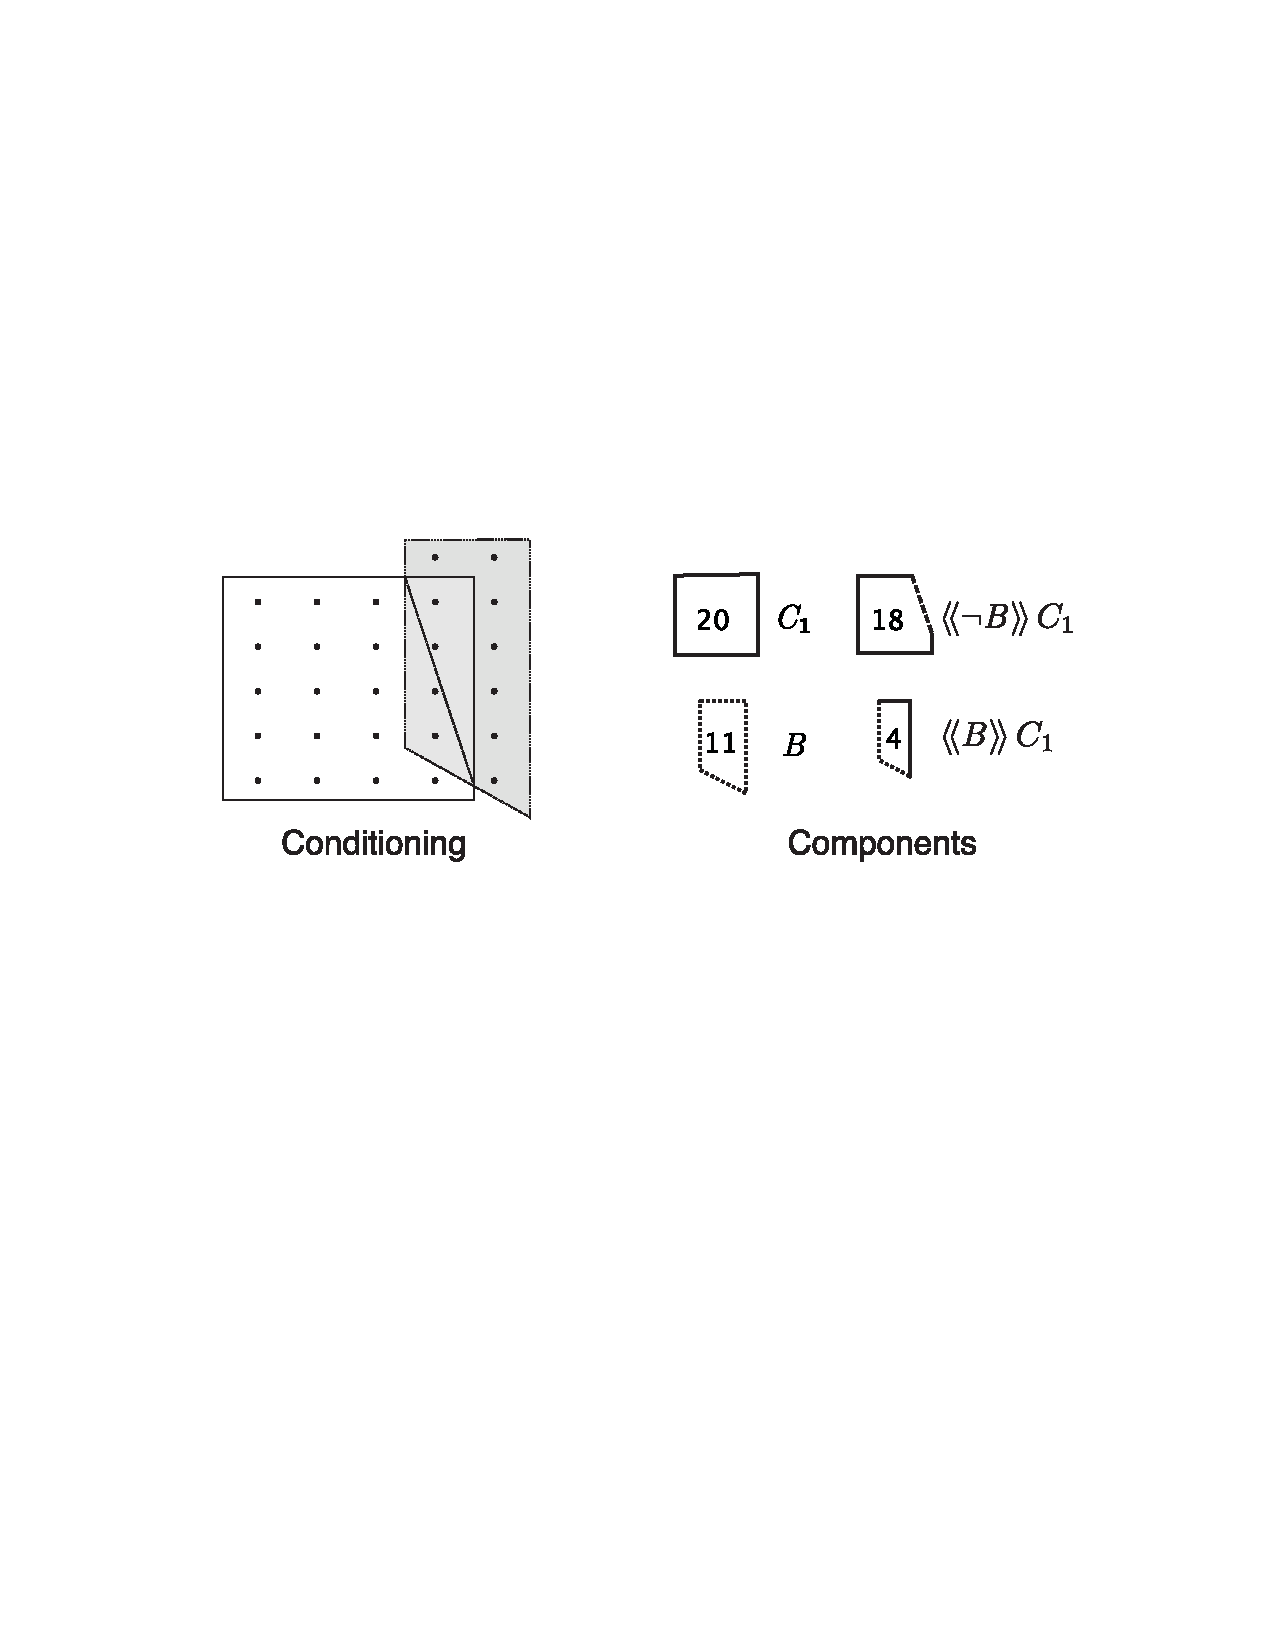
\includegraphics[width=7.5cm]{figures/conditioning-smaller.pdf}
\end{center}
\caption{\label{fig:conditioning} Example of distribution conditioning in the abstract domain $\ppolys$.}
\end{figure}

Figure \ref{fig:conditioning} demonstrates the components that affect the
conditioning operation.  The figure depicts the integer-valued points
present in two polyhedra---one representing $\getpoly{1}$ and the other
representing $\bexp$ (shaded).  As the set of points in $\getpoly{1}$
satisfying $\bexp$ is convex, 
this region is precisely represented by $\abseeval{\bexp}{\getpoly{1}}$.  By contrast, the set of points
in $\getpoly{1}$ that satisfy $\neg\bexp$ is not convex, and thus $\abseeval{\neg\bexp}{\getpoly{1}}$ is an
over-approximation.  The icons
beside the main image indicate which shapes correspond to which components
and the numbers within the icons give the total count of points within those
shapes.

Suppose the components of $\pp{1}$ are as follows.
\[
\begin{array}{l@{\qquad}l@{\qquad}l}
\smin{1} = 19 & \pmin{1} = 0.01 & \mmin{1} = 0.85 \\
\smax{1} = 20 & \pmax{1} = 0.05 & \mmax{1} = 0.9
\end{array}
\]
Then $n = 4$ and $\nn = 16$.  Note that we have set $\nn$ to be the
number of points in the non-shaded region of Figure \ref{fig:conditioning}.
This is more precise than the count given by $\psize{\abseeval{\bexp}{\poly}}$, which
would yield $18$.  This demonstrates why it is worthwhile to have a
separate operation for counting points satisfying a boolean expression.
These values of $n$ and $\nn$ give us the following for
the first four numeric components of $\pp{2}$.
\[
\begin{array}{l@{\qquad}l}
\smin{2} = \max(19 - 16, 0) = 3 & \pmin{2} = 0.01 \\
\smax{2} = \min(20,4) = 4 & \pmax{2} = 0.05
\end{array}
\]
For the $\mmin{2}$ and $\mmax{2}$, we have the following for the
method of calculation based on $\mathrm{p^{min/max}_2}$ and
$\mathrm{s^{min/max}_2}$.
\[
\begin{array}{l@{\qquad}l}
\mmin{2} = 0.01 \cdot 3 = 0.03  & \mmax{2} = 0.05 \cdot 4 = 0.2
\end{array}
\]
For the method of computation based on $\mathrm{m^{min/max}_1}$, we have
\[
\begin{array}{llcrr}
\mmin{2} &= &0.85 - 0.05 \cdot 16& =& 0.05\\
 \mmax{2} &= &0.9 - 0.01 \cdot (19-4)& =& 0.75
\end{array}
\]

In this case, the calculation based on subtracting from total mass
provides a tighter estimate for $\mmin{2}$, while the method based on
multiplying $\pmax{2}$ and $\smax{2}$ is better for
$\mmax{2}$.

\begin{lemma} \label{lem:pp:cond} If $ \delta \in \ppconc{\pp{}} $ then $
  \dcond{\delta}{B} \in \ppconc{\absdcond{\pp{}}{B}} $.
\end{lemma}


% \paragraph{Benefits of dual mass representations}

% The total minimum mass of a probabilistic polyhedron can seemingly be
% determined using two redundant means: either $ \mmin{} $ or $ \pmin{}\cdot \smin{} $. Tracking the measure in these two ways, however, is useful for
% keeping the measure accurate. For some abstract operations one of
% these means is more accurate than the other.

% Any abstract plus operation involving probabilistic polyhedra having
% two different minimum probability per point measures, the total mass
% based approach is more accurate, or equivalently accurate in the rare
% case where the minimum number of points is identical to the number of
% points in the polyhedra.

% \sbmcomment{It might be easier to read if we convert the fractions to decimals.}

% \begin{example} Consider two disjoint probabilistic polyhedra $ \ppa $, $ \ppb $,
% with the following characteristics:

% $ \pmin{1} = \frac{1}{100} $

% $ \smin{1} = 10 $

% $ \mmin{1} = \frac{10}{100} $

% $ \pmin{2} = \frac{1}{200} $

% $ \smin{2} = 20 $

% $ \mmin{2} = \frac{20}{100} $

% $ \pa \cap \pb = \emptyset $

% The abstract plus of the two, $ \ppc := \ppa \ppplus \ppb $ has the
% following properties.

% $ \pmin{3} = \frac{1}{200} $

% $ \smin{3} = 30  $

% $ \mmin{3} = \frac{30}{100} $

% Note that $ \pmin{3} \cdot \smin{3} = \frac{15}{100} $, a more inaccurate
% measure than $ \mmin{3} = \frac{30}{100} $.
% \end{example}

% The difference in the two total mass approaches stems from the need to
% under-approximate both minimum probability per point from both
% polyhedra with a single value.

% For abstract plus, the total mass approach always produces more
% accurate results but in the case of abstract revision, the approach
% can, in some cases, produce results worse than the $ \pmin{}\cdot \smin{} $ approach. First let us look at an example in which the total mass is
% still more accurate.

% \begin{example} Consider a probabilistic polyhedron $ \ppa $ and a
% polyhedron $ \pb $ where the intersection between the two is quite
% large in relation to the size of $ \pa $. 

% $ \pmin{1} = \frac{1}{1000} $

% $ \pmax{1} = \frac{1}{100} $

% $ \smin{1} = 95 $

% $ \mmin{1} = \frac{20}{100} $

% Furthermore, $ \setsize{\pa} - \setsize{\pa \cap \pb} = 10 $ and
% $ \setsize{\pa \cap \pb} = 90 $. That is, the $ \pa $ contains 100
% points, 90 of which are in the intersection with $ \pb $.

% To determine the total mass of $ \ppc := \absdcond{\ppa}{\pb} $ we
% reason that a maximum amount of mass falls outside the intersection,
% corresponding to $ \pmax{1} \cdot \paren{\setsize{\pa}
% - \setsize{\pa \cap \pb}} = \frac{1}{100} \cdot 10 $ .  \sbmcomment{I think you mean \textit{minimal} total mass here.}
% Thus the total
% mass of the intersection would be $ \mmin{1} - \frac{10}{100}
% = \frac{10}{100} $. On the other hand, $ \pmin{3} \cdot \smin{3}
% = \frac{1}{1000} \cdot 85 < \frac{10}{100} $.
% \end{example}

% As seen in the example above, the calculation of total mass derives
% it's accuracy from the maximum estimates as applied to the area
% outside of the intersection. If, however, this area is instead large,
% we see that this approach fails.

% \begin{example}

% Consider a probabilistic polyhedron $ \ppa $ and a
% polyhedron $ \pb $ where the intersection between the two is small in relation to the size of $ \pa $. 

% $ \pmin{1} = \frac{1}{1000} $

% $ \pmax{1} = \frac{1}{100} $

% $ \smin{1} = 95 $

% $ \mmin{1} = \frac{20}{100} $

% Furthermore, $ \setsize{\pa} - \setsize{\pa \cap \pb} = 90 $ and
% $ \setsize{\pa \cap \pb} = 10 $. That is, the $ \pa $ contains 100
% points, 10 of which are in the intersection with $ \pb $.

% To determine the total mass of $ \ppc := \absdcond{\ppa}{\pb} $ we
% reason that a maximum amount of mass falls outside the intersection,
% corresponding to $ \pmax{1} \cdot \paren{\setsize{\pa}
% - \setsize{\pa \cap \pb}} = \frac{1}{100} \cdot 90 $ . Thus the total
% mass of the intersection would be $ \mmin{1} - \frac{90}{100}
% = - \frac{70}{200} $, or simply a value having no use whatsoever. On the other hand, $ \pmin{3} \cdot \smin{3}
% = \frac{85}{1000} $. In such a case, we let $ \mmin{3}
% := \pmin{3} \cdot \smin{3} $ in order for the total mass measure to have
% potential usefulness in further computation.
% \end{example} 

\subsubsection{Scalar Product}
The scalar product is straightforward both in the concrete and
abstract sense; it just scales the mass per point and total mass:
$$ p \cdot \delta \defeq \lambda \sigma \lsep p \cdot \delta(\sigma) $$

\begin{definition}
Given a scalar $p$ in $(0,1]$, we write $p \cdot \ppa$ for the probabilistic polyhedron $\ppb$ specified below.
\[
\begin{array}{lcl@{\hspace{0.5cm}}|@{\hspace{0.5cm}}lcl}
\smin{2} &=& \smin{1} & \pmin{2} &=& p \cdot \pmin{1} \\
\smax{2} &=& \smax{1} & \pmax{2} &=& p \cdot \pmax{1} \\
\mmin{2} &=& p \cdot \mmin{1} & \getpoly{2} &=& \getpoly{1}\\
\mmax{2} &=& p \cdot \mmax{1} 
\end{array}
\]

If $ p = 0 $ then $ p \cdot \ppb $ is defined instead as below:
\[
\begin{array}{lcl@{\hspace{0.5cm}}|@{\hspace{0.5cm}}lcl}
\smin{2} &=& 0 & \pmin{2} &=& 0 \\
\smax{2} &=& 0 & \pmax{2} &=& 0 \\
\mmin{2} &=& 0 & \getpoly{2} &=& \pzero \\
\mmax{2} &=& 0 
\end{array}
\]
\end{definition}
Here $ \pzero $ refers to a convex polyhedra (over the same dimensions
as $ \getpoly{2} $) whose concretization is empty.

\begin{lemma}
\label{lem:pp:scalar-prod}
If $\delta_1 \in \ppconc{\pp{1}}$ then $p \cdot \delta_1 \in \ppconc{p \cdot \pp{1}}$.
\end{lemma}

\subsubsection{Normalization}
The normalization of a distribution produces a true probability
distribution, whose total mass is equal to $ 1 $:
$$ \normal{\delta} \defeq \frac{1}{\pmass{\delta}} \cdot \delta $$

If a probabilistic polyhedron $\pp{}$ has $\mmin{} = 1$ and $\mmax{} =
1$ then it represents a normalized distribution.  We define below an
abstract counterpart to distribution normalization, capable of
transforming an arbitrary probabilistic polyhedron into one containing
only normalized distributions.
% , with the property that if $\delta \in
% \ppconc{\pp{}}$ then $\normal{\delta} \in \ppconc{\normal{\pp{}}}$.
% This ensures that $\normal{\pp{}}$ is a sound over-approximation of
% $\normal{\delta}$ for the purposes of policy evaluation.

\begin{definition}
Whenever $ \mmin{1} > 0 $, we write $\normal{\pp{1}}$ for the
probabilistic polyhedron $\pp{2}$ specified below.
\[
\begin{array}{lcl@{\hspace{0.35cm}}|@{\hspace{0.35cm}}lcl}
\pmin{2} &=& \pmin{1} / \mmax{1} &
\smin{2} &=& \smin{1}\\
\pmax{2} &=& \pmax{1} / \mmin{1} &
\smax{2} &=&\smax{1} \\
\mmin{2} &=& \mmax{2} = 1 & \getpoly{2} &=& \getpoly{1} \\
\end{array}
\]
\end{definition}

When $ \mmin{1} = 0 $, we set $\pmax{2} = 1$.  Note that if $\pp{1}$
is the zero distribution then $\normal{\pp{1}}$ is not defined.

The normalization operator illustrates the key novelty of our
definition of probabilistic polyhedron: to ensure that the
overapproximation of a state's probability ($\pmax{}$) is sound, we
must divide by the \emph{underapproximation} of the total probability
mass ($\mmin{}$).

\begin{lemma}
\label{lem:pp:norm}
If $\delta_1 \in \ppconc{\pp{1}}$ and $\normal{\delta_1}$ is defined, then $\normal{\delta_1} \in \ppconc{\normal{\pp{1}}}$.
\end{lemma}

\subsection{Policy Evaluation}

\noindent Here we show how to implement the threshold test given as
Definition \ref{def:threshold} using probabilistic polyhedra. To make
the definition simpler, let us first introduce a bit of notation.

\begin{notation} If $ \pp{} $ is a probabilistic polyhedron over
  variables $ V $, and $ \sigma $ is a state over variables $ V'
  \subseteq V $, then $ \absdcond{\pp{}}{\sigma} \defeq
  \absdcond{\pp{}}{\bexp} $ where $ \bexp = \bigwedge_{x \in V'} x =
  \sigma(x) $.
\end{notation}

Recall that we define $\drevise{\delta}{\bexp}$ in the concrete
semantics to be $\normal{\dcond{\delta}{\bexp}}$.  The
corresponding operation in the abstract semantics is similar:
$\absdrevise{\pp{}}{\bexp} \defeq \normal{\absdcond{\pp{}}{\bexp}}$.

\begin{definition} \label{def:poly-threshold}
Given some probabilistic polyhedron $\pp{1}$ and statement $S$, with
low security variables $ L $ and high security variables $ H $, where
$\abspevalp{S}{\pp{1}} $ terminates, let $\pp{2} =
\abspevalp{S}{\pp{1}}$ and $\pp{3} = \project{\pp{2}}{L}$. If, for
every $ \sigma_L \in \pconc{\getpoly{3}} $ with $
\neg\iszero{\absdcond{\pp{2}}{\sigma_L}}$, we have $ \pp{4} =
\project{\paren{\absdrevise{\pp{2}}{\sigma_L}}}{H} $ with $\pmax{4}
\leq t$, then we write $\abspolicy{S}{\pp{1}}{t}$.
\end{definition}

The computation of $\pp{3}$ involves only abstract interpretation and
projection, which are computable using the operations defined previously
in this section.  If we have a small number of outputs (as for the binary outputs
considered in our examples), we can enumerate them and check
$\neg\iszero{\absdcond{\pp{2}}{\sigma_L}}$ for each output $\sigma_L$.
When this holds (that is, the output is feasible), we compute $\pp{4}$,
which again simply involves the abstract operations defined previously.
The final threshold check is then performed by comparing $\pmax{4}$ to
the probability threshold $t$.

Now we state the main soundness theorem for abstract interpretation
using probabilistic polyhedra.  This theorem states that the abstract
interpretation just described can be used to soundly determine whether
to accept a query.

\begin{theorem} \label{thm:pp:secure}
  Let $\delta$ be an attacker's initial belief.  If $\delta \in
  \ppconc{\pp{1}}$ and $\abspolicy{S}{\pp{1}}{t}$, then $S$ is threshold secure
  for threshold $t$ when evaluated with initial belief $\delta$.
\end{theorem}

The proof of this theorem follows from the soundness of the
abstraction (\tref{thm:pp:soundness}), noting the direct parallels of
threshold security definitions for distributions (Definitions
\ref{def:threshold}) and probabilistic polyhedra (Definition
\ref{def:poly-threshold}).

\subsection{Supporting Other Domains, Including Intervals and Octagons} \label{sec:simpler}

Our approach to constructing probabilistic polyhedra from normal
polyhedra can be adapted to add probabilities any other abstract
domain for which the operations defined in \sref{sec:polyhedra} can be
implemented.  Most of the operations listed there are standard to
abstract domains in general, except for the size operation and the
related expression count. Adopting an abstract domain to our system
would therefore only require designing these counting methods for the
new domain.

Two domains that are very easy to adapt that are in common use are
intervals and octagons.  \emph{Intervals} \cite{cousot76static},
$\intdomain$, are convex shapes that can be described as a set of
closed intervals, one for each dimension. Alternatively they can be
thought of a restricted form of polyhedra in which the constraints $I$
all have the form $ a \leq x \leq b $. Operations on intervals are
much faster than on polyhedra. Specific to our requirements, counting
the integer points inside interval regions and determining their
height for the forget operation are both trivial computations.

\emph{Octagons} \cite{mine01octagon}, $\octadomain$, are formed by
constraints $O$ that have the form $ a x + b y \leq c $ where $ a,b
\in \set{-1,0,1} $.  In two dimensions these shapes, appropriately,
have at most 8 sides. If the number of dimensions is fixed, the number
of constraints and the number of vertices of an octagon are
bounded. Furthermore, the operations on octagons have lower
computational complexity than those for polyhedra, though they are not
as efficient as those for intervals.

\begin{figure}
\begin{center}

\includegraphics[width=6.5cm]{figures/approx_domains.pdf} 
\end{center}
\caption{\label{fig:approx_domains} The (over)approximation of a polyhedron
  using an octagon (left) and an interval (right).}
\end{figure}

Any interval or octagon is also a polyhedron. Conversely, one can
over-approximate any polyhedron by an interval or octagon. Naturally
the smallest over-approximation is of greatest interest.
Examples are illustrated in \fref{fig:approx_domains}.  This fact is
relevant when computing the various equivalent operations to
those listed for polyhedra in Section~\ref{sec:polyhedra}: applying
the definitions given there on octagons/intervals may not necessarily
result in octagons/intervals, and so the result must be further
approximated.  For example, consider the evaluation operation $
\abseeval{\bexp}{I} $.  This must compute a region that contains \emph{at least}
the points in $ I $ satisfying $ \bexp $.  Thus, if a non-octagon/interval
is produced, it can simply be over-approximated.  Another example is
the affine
transform operation $ I \bparen{x \ra \aexp} $, which should
contain \emph{at least} the points $ \tau
= \sigma \bparen{x \ra \aexp} $ with $ \sigma \in \iconc{I} $, where
$ \sigma \bparen{x \ra \aexp} $ is a single state transformed by the
expression $ \aexp $. In general the operations for simpler domains
are much faster than those for more complex domains. Though the imprecision
and thus the need to approximate expression evaluation might
make it occasionally slower, for our experiments any slowdown is
typically overshadowed by the reduced complexity overall.

Thus we can construct abstractions of probability distributions based
on these simpler domains instead of polyhedra. The domain of
probabilistic intervals $ \pintdomain $ (octagons $ \poctadomain $)
is defined as in Section~\ref{def:ppoly}, except using an interval
(octagon) instead of polyhedron for the region constraint.  The
abstract semantics described in this section can then be soundly
implemented in terms of these simpler shapes in place of
polyhedra.

%We write $\ppolys$ for the set of probabilistic polyhedra.  The
%quantities $\smin{}$ and $ \smax{}$ are lower and upper bounds on 
%the number of support points in the polyhedron $\getpoly{}$.  The quantities
%$\pmin{} $ and $ \pmax{} $ are lower and upper bounds on the
%probability mass \emph{per support point}.  The $ \mmin{} $ and $
%\mmax{} $ components give bounds on the total probability mass.  
%Thus $\pp{}$ represents the \emph{set} of distributions
%$\ppconc{\pp{}}$ defined below. 

\begin{remark} If $ \delta \in \ppconc{\pp{}} $ then
$ \delta \in \piconc{\pint} $ and $ \delta \in \poconc{\pocta}
$, where $ \pint $ and $ \pocta $ are identical to $ \pp{} $
except $ \pp{} $ has region constrained by $ C $, a convex
polyhedron, while $ \pint $ is constrained by interval $ C_I $ and
$ \pocta $ is constrained by octagon $ C_O $, with
$ \pconc{C} \subseteq \iconc{C_I} $ and
$ \pconc{C} \subseteq \oconc{C_O} $.
\end{remark}

\section{Powerset of Probabilistic Polyhedra}
\label{sec:probset}

This section presents the $ \ppowers $ domain, an extension of the $ \ppolys
$ domain 
that abstractly represents a set of distributions as at most $ n $
probabilistic polyhedra, elements of $ \ppolys $.

\begin{definition} A \emph{probabilistic (polyhedral) set} $
  \pps{} $ is a set of probabilistic polyhedra, or  $ \set{\pp{i}} $
  with each $ \pp{i} $ over the same variables.\footnote{We write
    $\set{X_i}$ as shorthand for a set of $n$ elements of type $X$, for some
    $n$.  We write $\set{X_i}_{i=1}^{n}$ when the choice of
    $n$ is important.} We write $
  \ppowers $ for the domain of probabilistic polyhedral powersets
  composed of no more than $ n $ probabilistic polyhedra.

Each probabilistic polyhedron $\pp{}$ is interpreted disjunctively: it
characterizes one of many possible distributions.  The probabilistic
polyhedral set is interpreted additively.  To define this idea
precisely, we first define a lifting of $+$ to sets of distributions.  Let $\distset{1}, \distset{2}$ be two sets of distributions.  We then define addition as follows.
\[\distset{1} + \distset{2} = \{\delta_1 + \delta_2 \given \delta_1 \in \distset{1} \wedge \delta_2 \in \distset{2}\}\]
This operation is commutative and associative and thus we can use
$\sum$ for summations without ambiguity as to the order of operations.
The concretization function for $\ppowers$ is then defined as:
$$ \ppsconc{\pps{}} \defeq \sum_{\pp{} \in \pps{}} \ppconc{\pp{}} $$
\end{definition}

Following Monniaux's formulation of a finite sums
abstraction~\cite{Monniaux_these}, elements of $ \pps{} $ need not be
disjoint. While enforcing disjointness would simplify determining the 
most probable points for policy evaluation (see
\sref{sec:poly-eval}), it would necessitate splitting of probabilistic
polyhedra when overlaps arise.  Repeated splitting of already
approximate probabilistic polyhedra decreases their
precision and can hurt performance by increasing the number of regions
to track during abstract interpretation.

We can characterize the condition of $ \pps{} $ containing only the
zero distribution, written $ \iszero{\pps{}} $, via the condition that
all of the member probabilistic polyhedra are zero.
$$ \iszero{\pps{}} \defeq \bigwedge_{\pp{} \in \pps{}} \iszero{\pp{}} $$

\deleted{
\begin{definition} $ \delta_a = \delta_b $ if and only if $ \forall \sigma $ $
  \delta_a(\sigma) = \delta_b(\sigma) $.
\end{definition}
}

\subsection{Abstract Semantics for $\ppowers$} \label{sec:powerset}
The semantics for the powerset abstraction we describe in this section
is designed to soundly approximate the concrete semantics. 

\begin{theorem} \label{thm:ppp:soundness}
For all $\delta, S, \pps{}$, if $\delta \in \ppsconc{\pps{}}$ and $
\abspevalp{S}{\pps{}} $ terminates, then $ \pevalp{S}{\delta} $ terminates and
$\pevalp{S}{\delta} \in
\ppsconc{\abspevalp{S}{\pps{}}}$.
\end{theorem}

The proof for this theorem follows the same form as the corresponding
soundness theorem for probabilistic polyhedra
(\tref{thm:pp:soundness}), via soundness of the individual abstract
operations in relation to their concrete versions. The full proof of
this is given in the companion technical
report~\cite{TR}.

To bound the size of the set of probabilistic polyhedra that
will arise from the various operations that will follow, we introduce a
simplification operation.

\begin{definition}
\label{def:ppp-simp}
The \emph{powerset simplification} transforms a
  set containing potentially more than $ n $ elements into one
  containing no more than $ n $, for $n \geq 1$. The simplest approach involves repeated use
  of abstract plus in the base domain $ \ppolys $.
$$
\simplify{\set{\pp{i}}_{i=1}^{m}}{n} \defeq \left\{
\begin{array}{cc}
\set{\pp{i}}_{i=1}^{m} & \text{if } m \leq n \\
\simplify{\set{\pp{i}}_{i=1}^{m-2} \cup \set{\pp{m-1} + \pp{m}}}{n} & \text{otherwise} \\
\end{array}
\right.
$$
\end{definition}

\begin{lemma}
\label{lem:ppp:bound}
$ \ppsconc{\pps{}} \subseteq \ppsconc{
    \simplify{\pps{}}{m}} $ where $m \leq n$.
\end{lemma}

Note that the order in which individual probabilistic polyhedra are
simplified has no effect on soundness but may impact the precision of
the resulting abstraction. We explore the variation in precision due
to these choices in \sref{sec:perf-analysis}.

Many of the operations and lemmas for the powerset domain are simple liftings
of the corresponding operations and lemmas for single probabilistic polyhedra.
For these operations (the first four, below) we simply list the
definition; we elaborate on the remaining four.

\paragraph{Forget} $ \forget{y}{\pps{}} \defeq
\set{\forget{y}{\pp{}} \given \pp{} \in \pps{}} $

\vspace*{.1in}
\noindent
\myparagraph{Project} $ \project{\pps{}}{V} \defeq
\set{\project{\pp{}}{V} \given \pp{} \in \pps{}} $

% \begin{lemma} 
% If $ \delta \in \ppsconc{\pps{}} $ then $
%   \project{\delta}{\paren{\fv{\delta} - \set{y}}} \in
%   \ppsconc{\forget{y}{\pps{}}} $
% \end{lemma}

\vspace*{.1in}
\noindent
\myparagraph{Assignment} $ \pps{} \bparen{x \ra E} \defeq
  \set{\pp{} \bparen{x \ra E} \given \pp{} \in \pps{}} $

% \begin{lemma} If $ \delta \in \ppsconc{\pps{}} $ then $
%   \delta\bparen{x \ra E} \in \ppsconc{\pps{} \bparen{x \ra E}} $.
% \end{lemma}

\vspace*{.1in}
\noindent
\myparagraph{Scalar product} $ p \cdot \pps{} \defeq \set{p
  \cdot \pp{} \given \pp{} \in \pps{} \wedge \neg \iszero{p \cdot \pp{}}} $

% \begin{lemma} If $ \delta \in \ppsconc{\pps{}} $ then $
%   p \cdot \delta \in \ppsconc{p \cdot \pps{}} $.
% \end{lemma}

\paragraph{Conditioning}
Recall that for probabilistic polyhedra, conditioning $
\absdcond{\pp{}}{\bexp} $ is defined in terms of logical expression
evaluation for convex polyhedra, $ \abseeval{\bexp}{\poly} $. This
operation returns a convex polyhedron that contains at least the points
in $ \poly $ that satisfy the logical expression $ \bexp $. This
operation is tight if $ \bexp $ does not contain disjuncts.  When
$ \bexp $ does have disjuncts whose union does not define
a convex region then the operation will be approximate.  Consider
Example~\ref{ex:specyear}. The condition 
$ \var{age} = 20 \vee \var{age} = 30 \vee ... \vee \var{age} = 60 $,
were it be approximated using a single convex region, would be
equivalent to the condition $ \var{age} \geq 20 \vee \var{age} \leq 60
$.

In the powerset domain we keep track of multiple convex regions hence
can better approximate the conditioning operation. The approach we
take is to convert the logical expression into a \emph{disjoint}
disjunctive normal form: $ \ddnf{\bexp} \defeq \set{B_1, B_2, \cdots,
  B_m} $, such that $ \set{\sigma \given \sigma \models \bexp} = \set{\sigma
  \given \sigma \models \bexp_1 \vee \cdots \vee \bexp_m} $, each
disjunct $ \bexp_i $ contains no further disjunctions, and $
\set{\sigma \given \sigma \models \bexp_i \wedge \bexp_j} = \emptyset
$ for all $ i \neq j $ ($ B_i $ are disjoint).
%such that $ \bexp \models \ismodeledby \paren{\bexp_1 \vee
%  \bexp_2 \vee \cdots \vee \bexp_m} $, each disjunct $ B_i $ contains
%no further disjunctions, and $ B_i \wedge B_j \models \bot $ for all
%$j \not= i$ (i.e., all $B_i$ are disjoint).

Conditioning is thus defined as follows:
$$ \absdcond{\pps{}}{\bexp} \defeq
\simplify{\set{\absdcond{\pp{}}{\bexp_i} \given \pp{} \in \pps{} \wedge \bexp_i
  \in \ddnf{\bexp} \wedge \neg \iszero{\absdcond{\pp{}}{\bexp_i}}}}{n} $$

The powerset simplification here reduces the set
of probabilistic polyhedra to no more than $ n $. Before the
simplification, the number of probabilistic polyhedra could be as
large as $ \setsize{\pps{}} \cdot \setsize{\ddnf{\bexp}} $. The number of
disjuncts itself can be exponential in the size of $ \bexp $.

\paragraph{Product} The product operation is only required for the
special $ \suniformname $ statement and only applies to the product
of a probabilistic set with a single probabilistic polyhedron.
$ \pps{} \times \pp{}' \defeq \set{\pp{} \times \pp{}' \given \pp{} \in \pps{}} $
(where we assume that $\fv{\pps{}} \cap \fv{\pp{}'} = \emptyset$).

% \begin{lemma} If $ \delta_a \in \ppsconc{\pps{}} $ and $ \delta_b \in
%   \ppconc{\pp{}'} $ then $
%   \delta_a \times \delta_b \in \ppsconc{\pps{} \times \pp{}'} $.
% \end{lemma}

% As we did with the base domain, we take advantage of the extra $
% \suniformname $ statement introduced into the language, we handle its
% abstract interpretation in a specific way.

% $$
% \begin{array}{rcl}
% \abspevalp{\suniform{x}{n_1}{n_2}}{\pps{}} & = &
% \forget{x}{\pps{}} \times \pp{2}
% \end{array}
% $$

% Where $ \pp{2} $ has $ \pmin{2} = \pmax{2} = \frac{1}{n_2 - n_1 + 1}
% $, $ \smin{2} = \smax{2} = n_2 - n_1 + 1 $, $ \mmin{2} = \mmax{2} = 1
% $, and $ C_2 = \set{x \geq n_1, x \leq n_2} $.

\paragraph{Plus} The abstract plus operation involves simplifying
the combined contributions from two sets into one bounded set:
$ \pps{1} + \pps{2} \defeq \simplify{\pps{1} \cup \pps{2}}{n} $,
whenever $ \neg\iszero{\pps{1}} $ and $ \neg\iszero{\pps{2}}
$. Alternatively, if $ \iszero{\pps{1}} $ (or $ \iszero{\pps{2}} $)
then $ \pps{1} + \pps{2} $ is defined to be identical to $
\pps{2} $ (or $ \pps{1} $).

The definition of abstract plus given above is technically sound but
for an implementation it would make sense to assuming that $ \pps{1} $
contains probabilistic polyhedra that are somewhat more related to
each other than those in $ \pps{2} $. It is preferable to merge
regions that close together rather than those further apart. Therefore
our implementation performs abstract plus heuristically as
follows.
$$ \pps{1} + \pps{2} = \simplify{\pps{1}}{\floor{n/2}} \cup
\simplify{\pps{2}}{n - \floor{n/2}} $$ This may not always be the best
grouping of probabilistic polyhedra to merge. There is quite a lot of
arbitrary choice that can be made in order to evaluate this heuristic
or the base definition of abstract plus without this heuristic.

\deleted{
\subsubsection{Conditioning} To take best advantage of the richer
abstraction, we can approximate the state cover of boolean expressions
using a set of polyhedra interpreted as disjuncts, called the
\emph{disjunctive abstract}, and then condition
on this set rather than on single polyhedron.
\begin{definition}
A set of convex polyhedra $ \polyset $ represents all states that
are in at least one of its the polyhedra.
$ \psconc{\polyset} \defeq \bigcup_{\poly \in \polyset} \pconc{\poly} $
\end{definition}
\begin{definition} The \emph{disjunctive abstract} of a boolean expression
  $\bexp$, denoted $ \absdbexp{m}{\bexp} $, is a set of polyhedra $
  \polyset $ with $ \setsize{\polyset} \leq m $, and $
  \set{\sigma \given \sigma \models B} \subseteq  \psconc{\polyset} $.
\end{definition}

Thus, to compute $ \absdcond{\pps{}}{\bexp} $ we simply compute $
\absdcond{\pps{}}{\polyset} $ defined as follows, where $\polyset =
\absdbexp{m}{\bexp}$.
\begin{definition} Conditioning a single probabilistic polyhedron
  $\pp{}$ on a $\polyset$, which produces a
member of $ \ppowers$, is defined as follows:
$ \absdcond{\pp{1}}{\polyset} \defeq \bigcup_{\poly \in \polyset}
\absdcond{\pp{1}}{\poly} $.  Conditioning a set $\pps{}$ on $\polyset$
can then be defined as:
$ \absdcond{\pps{}}{\polyset} \defeq \bigsimplify{\bigcup_{\pp{i} \in \pps{}}
\bigl(\absdcond{\pp{i}}{\polyset}\bigr)}{n} $.
\end{definition}
Note that the parameter $ m $ bounding the number of disjuncts in the
abstraction of $\bexp$ need not be related to $ n $.

\begin{lemma}
\label{lem:ppp:cond}
If $ \delta \in \ppsconc{\pps{}} $ then $
  \dcond{\delta}{B} \in \ppsconc{\absdcond{\pps{}}{B}} $.
\end{lemma}
}

\paragraph{Normalization} 

Since in the $ \ppowers $ domain the over(under) approximation of the
total mass is not contained in any single probabilistic polyhedron,
the normalization must scale each component of a set by the overall
total. The minimum (maximum) mass of a probabilistic polyhedron set
$\pps{} = \{\pp{1},\ldots,\pp{n}\}$ is defined as follows.
$$\begin{array}{l|l}
\ppmmin{\pps{}} \defeq \sum_{i=1}^n \mmin{i}\quad &\quad
\ppmmax{\pps{}} \defeq \sum_{i=1}^n \mmax{i} \\
\end{array}$$

\begin{definition}

\newcommand{\munder}{\underline{m}}
\newcommand{\mover}{\overline{m}}

The normalization a probabilistic polyhedra $ \pp{1} $ relative to a
probabilistic polyhedron set $ \pps{} $, written $
\normalp{\pps{}}{\pp{1}} $, is the probabilistic polyhedron $ \pp{2} $
defined as follows whenever $ \ppmmin{\pps{}} > 0 $.
\[
\begin{array}{lcl@{\hspace{0.35cm}}|@{\hspace{0.35cm}}lcl}
\pmin{2} &=& \pmin{1} / \ppmmax{\pps{}} &
\smin{2} &=& \smin{1}\\
\pmax{2} &=& \pmax{1} / \ppmmin{\pps{}} &
\smax{2} &=&\smax{1} \\
\mmin{2} &=& \mmin{1} / \ppmmax{\pps{}} & \getpoly{2} &=& \getpoly{1} \\
\mmax{2} &=& \mmax{1} / \ppmmin{\pps{}} \\
\end{array}
\]

Whenever $ \ppmmin{\pps{}} = 0 $ the resulting $ \pp{2} $ is defined
as above but with $\pmax{2} = 1$ and $\mmax{2} = 1$.
\end{definition}

Normalizing a set of probabilistic polyhedra is then defined as follows
$$ \normal{\pps{}} \defeq \set{\normalp{\pps{}}{\pp{}} \given \pp{} \in
  \pps{}} $$

%\begin{definition} We write $\maxprobof{\pp{}}{\sigma}$ to mean the maximum
%  probability of a state $ \sigma $ according to a \ppname{} $ \pp{} $, and
%  $\maxprobof{\pps{}}{\sigma}$ to mean the maximum probability of a
%  state $\sigma$ according to a \ppsname{} $\pps{}$.  The definitions
%  are as follows. 
%$$
%\begin{array}{l|l}
% \maxprobof{\pp{}}{\sigma} = \left\{ \begin{array}{cc}
%\pmax{} & \text{if } \sigma \in \pconc{\getpoly{}} \\
%0        & \text{otherwise} \\
%\end{array} \right. \quad & \quad
%\maxprobof{\pps{}}{\sigma} = \sum_i \maxprobof{\pp{i}}{\sigma} \\
%\end{array}
%$$
%
%\end{definition}

\subsubsection{Powersets of Intervals and
  Octagons} \label{sec:psimpler}

Following the probabilistic extensions to the interval and octagon
domains described in Section~\ref{sec:simpler}, we can also define
powersets of probabilistic intervals and octagons: $ \ppintdomain $ is
composed of at most $ n $ probabilistic intervals and $ \ppoctadomain
$ is composed of at most $ n $ probabilistic octagons.  The
operations have the same form as those described above.

\subsection{Policy Evaluation}
\label{sec:poly-eval}

Determining the bound on the probability of any state represented by a
single \ppname{} is as simple as checking the $ \pmax{} $ value in the
normalized version of the \ppname{}. In the domain of \ppsnames{},
however, the situation is more complex, as polyhedra may overlap and
thus a state's probability could involve multiple \ppnames{}.
A simple estimate of the bound can be computed by abstractly adding all the 
\ppnames{} in the set, and using the $ \pmax{} $ value of the
result.

\begin{lemma}
\label{lem:ppp:prob-bound}
%Let $\pp{} = \paren{\Sigma_i \pp{i}}$.  Then
%$ \maxprobof{\pps{}}{\sigma} \leq
%  \maxprobof{\pp{}}{\sigma} $
If $ \delta \in \ppsconc{\pps{}} $ and $ \pp{1} = \sum_{\pp{} \in \pps{}} \pp{}
$ then $ \max_{\sigma} \delta(\sigma) \leq \pmax{1} $.
\end{lemma}

This approach has an unfortunate tendency to increase the max probability
bound as one increases the bound on the number of
probabilistic polyhedra allowed.  A more complicated method, which is
used in our implementation, computes a partition of the polyhedra in
the set into another set of disjoint polyhedra and determines the
maximum probable point among the representatives of each region in the
partition. In order to present this method precisely we begin with
some definitions. 

\begin{definition} \label{def:max_prob} The \emph{maximum} probability of a state $ \sigma $ according to
a probabilistic polyhedron $ \pp{1} $, written $
\ppprob{\pp{1}}{\sigma} $, is as follows.
%$ \pmax{1} $ if $ \pp{1} \in
%\pconc{\getpoly{1}} $ and $ 0 $ otherwise.
$$ \ppprob{\pp{1}}{\sigma} \defeq \left\{
   \begin{array}{ll}
   \pmax{1} & \text{if } \sigma \in \pconc{\getpoly{1}} \\
   0        & \text{otherwise}
\end{array}
\right.
$$

Likewise the \emph{maximum} probability of $ \sigma $ according to a
probabilistic polyhedron set $ \pps{} = \set{\pp{i}} $, written $
\ppsprob{\pps{}}{\sigma} $, is defined as follows.
$$ \ppsprob{\pps{}}{\sigma} \defeq \sum_i \ppprob{\pp{i}}{\sigma} $$
\end{definition}

A mere application of the various definitions allows one to conclude
the following.

\begin{remark} \label{rem:ppp:prob} If $ \delta \in \ppsconc{\pps{}} $ then
for every $ \sigma $, $ \delta(\sigma) \leq \ppsprob{\pps{}}{\sigma}
$, and therefore $ \max_{\tau} \delta(\tau) \leq
\max_{\tau}\ppsprob{\pps{}}{\tau} $.
\end{remark}

Notice that in the case of a single probabilistic polyhedron, $
\ppprob{\pp{1}}{\sigma} = \ppprob{\pp{1}}{\tau} $ for every $ \sigma,
\tau \in \pconc{\getpoly{1}} $. That is, every supported state has the
same maximum probability. On the other hand, this is not the case for
sets of probabilistic polyhedra, $ \ppsprob{\pps{}}{\sigma} $ is not
necessarily equal to $ \ppsprob{\pps{}}{\tau} $, for supported states
$ \sigma, \tau \in \bigcup_{\pp{i}\in\pps{}} \pconc{\getpoly{i}} $, or
even for states $ \sigma, \tau \in \pconc{\getpoly{i}} $, supported by
a single probabilistic polyhedron $ \pp{i} \in \pps{} $. This is the
case as there might be one set of probabilistic polyhedra in $ \pps{}
$ that supports a state $ \sigma $, while a different set supports $
\tau $.

Taking advantage of the polyhedra domain, we will produce a set of
representative points $ \set{\sigma_j}_{j=1}^{m} $ with $
\max_{j=1}^{m}\ppsprob{\pps{}}{\sigma_j} =
\max_{\sigma}\ppsprob{\pps{}}{\sigma} $. This set will thus let us
determine the maximum probability over all points, without having to
look at all points. To do this, we first need to define a linear
partition. 

\begin{definition} \label{def:ppp:pp} A \emph{poly partition} of a set of polyhedra
$ \set{P_i}_{i=1}^{n} $ is another set of polyhedra $ \set{L_j}_{j=1}^{m} $, usually of
larger size, with the following properties.

\begin{enumerate}
\item{} $ \pconc{L_i} \cap \pconc{L_j} = \emptyset $
for every $ i \neq j $.
\item{} $ \cup_{j=1}^{m} \pconc{L_j} = \cup_{i=1}^{n} \pconc{P_i} $
\item{} For every $ i,j $, either $ \pconc{L_i} \subseteq \pconc{P_j}
$ or $ \pconc{L_i} \cap \pconc{P_j} = \emptyset $.
\end{enumerate}

\begin{figure}
\begin{center} 
\includegraphics[width=6.5cm]{figures/poly_partition.pdf} \end{center}
\caption{\label{fig:poly-partition} Example of a poly partition of two
  overlapping convex polyhedra (shaded), resulting in 5 disjoint convex polyhedra
  (outlined).}
\end{figure}

We call any set $R = \set{\sigma_j}_{j=1}^{m} $  a \emph{representative set}
of partition $ \mathcal{L} = \set{L_j}_{j=1}^{m} $ when the $j$th
element $\sigma_j \in R$ is in the concretization of the respective element $L_j
\in \mathcal{L}$; i.e., $ \sigma_j \in \pconc{L_j}$. 

\end{definition}

We can now determine the maximal probability using only representative
points, one from each piece of the poly partition.

\begin{lemma} \label{lem:ppp:pp} $ \max_{\sigma \in R}\ppsprob{\pps{}}{\sigma}
= \max_{\sigma}\ppsprob{\pps{}}{\sigma} $ where $ \parta $ is a poly
partition of $ \pps{} $ and $ R $ is a representative set
of $ \parta $. 
\end{lemma}

Note that the set of representatives $ R $ is not unique and the lemma
holds for any such set and the maximal state probability is the same,
regardless of which set of representatives is used, or even which poly
partition is computed. Also note that the process of producing the
poly partition would be unnecessary if somehow we kept the regions
defined by probabilistic polyhedra in $ \pps{} $ disjoint from each
other, as they would already define a poly partition. Doing so would
simplify our task here, but would significantly complicate matters in
the abstract interpretation of a program, as well as reducing the
precision of the final result.

The process of producing a poly partition
from a set of polyhedra is achieved via repeated use of the linear
partition operation for polyhedra, which splits two polyhedra into
disjoint pieces. Our implementation does this in the most naive way
possible: we maintain a bag of polyhedra, splitting any overlapping
pairs, until no overlapping regions remain, as in the pseudo-code
below.
\begin{align*}
& \var{poly}\text{-}\var{partition}(\Phi) \defeq \\
& \;\; \awhile \; \exists \; \pa, \pb \in \Phi \given \neg \isempty{\pa \pmeet
   \pb} \\
& \;\;\;\; \Phi \leftarrow \paren{\Phi-\set{\pa,\pb}} \cup
  \paren{\partn{\pa}{\pb}} \\
& \;\; \areturn \; \Phi
\end{align*}

We will write $ \ppsmax{\pps{}} $ for $
\max_{\sigma}\ppsprob{\pps{}}{\sigma} $ to make explicit the method
with which this value can be computed according to the lemma above.

\begin{notation} If $ \pps{} $ is a probabilistic polyhedron set over
  variables $ V $, and $ \sigma $ is a state over variables $ V'
  \subseteq V $, then $ \absdcond{\pps{}}{\sigma} \defeq
  \absdcond{\pps{}}{\bexp} $ where $ \bexp = \bigwedge_{x \in V'} x =
  \sigma(x) $.
\end{notation}

%To describe policy evaluation we begin by defining concretization for
%sets of polyhedra.
%\noindent
%We now define $\abspolicyname$ for $\ppowers$:
%
%\begin{definition}
%Suppose we have some initial probabilistic polyhedron set $\pps{1} $.
%Let $\pps{2} = \abspevalp{S}{\pps{1}}$.  Let $\pps{}' = \set{\pp{i}'} =
%\project{\pps{2}}{L} $.  If, for all $ \sigma \in
%\psconc{\set{\getpoly{i}'}} $ we have $\maxprobof{\pps{3}}{\sigma}
%\leq t$ where $\pps{3} = \normal{\absdcond{\pps{2}}{\bigwedge_{x \in L} x =
%    \sigma(x)}}$, then we write $\abspolicy{S}{\pps{1}}{t}$.
%\end{definition}

\begin{definition}
Given some probabilistic polyhedron set $\pps{1}$ and statement $ S $ where
$ \abspevalp{S}{\pps{1}} $ terminates, let $\pps{2} =
\abspevalp{S}{\pps{1}}$ and $\pps{3} = \project{\pps{2}}{L} =
\set{\pp{i}'}$. If for every $ \sigma_L \in \psconc{\set{\poly_{i}'}} $
with $ \neg\iszero{\absdcond{\pps{2}}{\sigma_L}} $ we have $ \pps{4} =
\project{\paren{\absdrevise{\pps{2}}{\sigma_L}}}{H} $ and
$ \ppsmax{\pps{4}} \leq t $, then we write
$\abspolicy{S}{\pps{1}}{t}$.
\end{definition}

Below we state the main soundness theorem for abstract interpretation
using \ppsnames{}.  This theorem states that the abstract
interpretation just described can be used to soundly determine whether
to accept a query.

\begin{theorem}
\label{thm:ppp:secure}
  Let $\delta$ be an attacker's initial belief.  If $\delta \in
  \ppsconc{\pps{}}$ and $\abspolicy{S}{\pps{}}{t}$, then $ S $ is threshold secure
  for threshold $t$ when evaluated with initial belief $\delta$.
\end{theorem}

Note that the process described in computing
threshold security involves merging probabilistic polyhedra via the simplification
operation (Definition~\ref{def:ppp-simp}); the
order in which these polyhedra are combined has no effect on
soundness, but could affect precision. 
We explore the variation possible in the precision due to ordering in
\sref{sec:perf-analysis}. The heuristic used for simplification in the
abstract plus operation aims to optimize some of these choices;
further optimizations are part of our ongoing work.

% Examples from talk on 1/7/2011
% DHS <- Airline
% CIA <-> MI6
% Realty A <-> Realty B (to find double-dealing sellers
% IRS <- Swiss Bank (to find info on suspected tax cheats)
% Hospital <- Social Security Administration (# patients with fake SSNs)
% Alice <-> Bob (do we have at least k friends in common?)

%\mwh{We need this stuff, but not sure where it goes yet:}
%
%In the static analysis we develop, we will work with representations
%of sets of distributions.  There are operations analogous to those
%above operating on such sets.  Suppose $D_1,D_2$ are sets of
%distributions.  Then we have the following.  We re-use the notation
%introduced above when the operation is a simple lifting of the
%corresponding operation on distributions.  Whether the operation is
%being applied to distributions or sets of distributions will always be
%clear from context.
%
%\begin{itemize}
%\item{} \emph{minimum distribution mass} -- The \emph{minimum mass} of a set of distributions,
%  $ \pmassmin{D_1} $ is $\min\{\pmass{\delta} \given \delta \in D_1\}$.
%
%\item{} \emph{maximum distribution mass} -- The \emph{maximum mass} of a set of distributions,
%  $ \pmassmax{D_1} $ is $\max\{\pmass{\delta} \given \delta \in D_1\}$.
%
%\sbmcomment{May not end up using the above two.}
%
%\item{} \emph{normalized distribution} -- A set of distributions is \emph{normalized}
%  if and only if every component distribution is normalized.
%
%\item{} \emph{distribution product} -- \sbmcomment{Left out because I don't think we use it.}
%
%\item{} \emph{distribution revision} -- 
%$\dcond{D_1}{S} = \{ \dcond{\delta}{S} \given \delta \in D_1 \}$
%
%\item{} \emph{distribution scalar product} -- Given a
%  scalar $ p $ in $ [0,1] $, we have
%
%$ p \cdot D_1 = \{ p \cdot \delta \given \delta \in D_1 \} $
%
%\item{} \emph{distribution normalization} --
%$ \normal{D_1} = \{\normal{\delta} \given \delta \in D_1\}$
%
%\item{} \emph{distribution sum} -- 
%$D_1 + D_2 = \{\delta_1 + \delta_2 \given \delta_1 \in D_1 \wedge \delta_2 \in D_2\} $
%\end{itemize}

%\subsection{Powersets of Intervals and Octagons} \label{sec:psimpler}
%
%To balance the precision loss due to the simpler domains, we increase
%the number of probabilistic regions in a powerset representation,
%though of course still maintaining the upper bound on their
%number. Specifically, the abstract interpretation of the $ \suniformname $
%statement produces two regions instead of one.  \mwh{Explain why doing
%  this will help precision}
%
%Specifically, the statement $\suniform{x}{n_1}{n_2}$ has the following
%abstract semantics (in the case of probabilistic intervals).
%$$
%\begin{array}{rcl}
%\abspevalp{\suniform{x}{n_1}{n_2}}{\pps{}} & = & \forget{x}{\pps{}}
%\times I_1 + \forget{x}{\pps{}} \times I_2
%\end{array}
%$$
%If we let $ m = \floor{\frac{n_1+n_2}{2}} $, then the parameters of
%the two probabilistic intervals $ I_1, I_2 $ above are as follows.
%$$
%\begin{array}{lr}
%\pmin{1} = \pmax{1} = \frac{1}{n_2 - n_1 + 1} & \pmin{2} = \pmax{2}
%= \frac{1}{n_2 - n_1 + 1} \\
%\smin{1} = \smax{1} = m - n_1 + 1  & \smin{2} = \smax{2} = n_2 - m \\
%\mmin{1} = \mmax{1} = \frac{m - n_1 + 1}{n_2 - n_1 + 1} & \mmin{2} = \mmax{2} = \frac{n_2 - m}{n_2 - n_1 + 1} \\
%{C_I}_1 = (\set{x \geq n_1, x \leq m}, \set{x}) & {C_I}_2 = (\set{x \geq m+1, x \leq n_2}, \set{x})\\
%\end{array}
%$$
%
%Though we split our uniform regions in two, we could just have well
%split them into more than two. Ideally regions could be split only
%when necessary and in the face of particularly unrepresentable
%inequalities.

\begin{figure}[t]
\centering
\begin{tabular}{c}
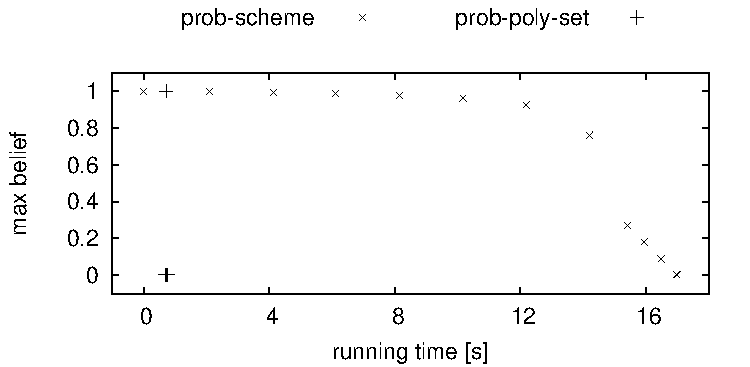
\includegraphics[width=9cm]{figures/plot_bday.pdf} \\
(a) birthday query (\eref{ex:bday}) \\
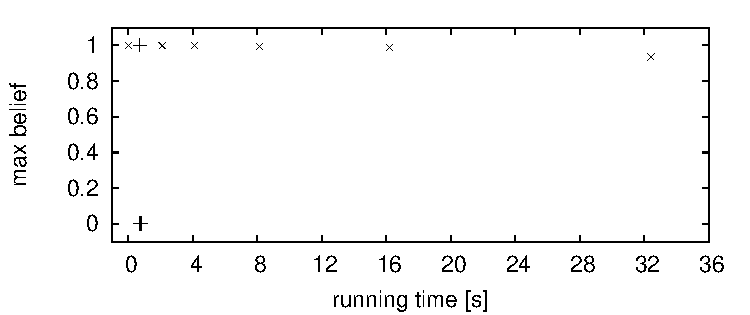
\includegraphics[width=9cm]{figures/plot_bday_large.pdf} \\
(b) birthday query (\eref{ex:bday}), larger state space \\
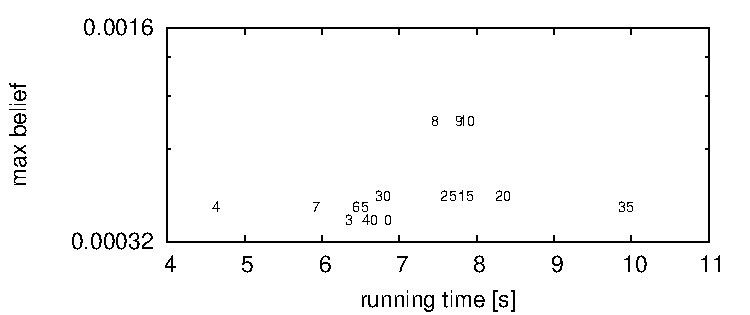
\includegraphics[width=9cm]{figures/plot_bday_seq.pdf} \\
(c) special year query (\eref{ex:specyear}) \\
\end{tabular}
\caption{Query evaluation comparison}
\label{fig:plots_bday}
\end{figure}

\iffull
\begin{table*}[t]
\scriptsize
\centering
\begin{tabular}{||p{1.35cm}|p{0.50cm}p{0.50cm}p{0.50cm}p{0.50cm}p{0.50cm}p{0.50cm}p{0.50cm}p{0.50cm}p{0.50cm}p{0.50cm}p{0.50cm}p{0.50cm}p{0.50cm}p{0.50cm}p{0.50cm}p{0.50cm}p{0.50cm}c||}
\hline \hline {\small time [s]} \par {\scriptsize max belief}& \multicolumn{18}{c||}{\textbf{prob-poly set size bound}} \\
\hline \hline \textbf{query} & \textbf{1} & \textbf{2} & \textbf{3} & \textbf{4} & \textbf{5} & \textbf{6} & \textbf{7} & \textbf{8} & \textbf{9} & \textbf{10} & \textbf{15} & \textbf{20} & \textbf{25} & \textbf{30} & \textbf{35} & \textbf{40} & \textbf{$ \infty $} & \\
\hline \hline bday \par 1 box & {\small 0.0}\par{\scriptsize\parbox{1.0cm}{1}} \par{\scriptsize 0} & {\small 0.0}\par{\scriptsize\parbox{1.0cm}{0.00386}} \par{\scriptsize 0} & {\small 0.0}\par{\scriptsize\parbox{1.0cm}{0.00386}} \par{\scriptsize 0} & {\small 0.0}\par{\scriptsize\parbox{1.0cm}{0.00386}} \par{\scriptsize 0} & {\small 0.0}\par{\scriptsize\parbox{1.0cm}{0.00386}} \par{\scriptsize 0} & {\small 0.0}\par{\scriptsize\parbox{1.0cm}{0.00386}} \par{\scriptsize 0} & {\small 0.0}\par{\scriptsize\parbox{1.0cm}{0.00386}} \par{\scriptsize 0} & {\small 0.0}\par{\scriptsize\parbox{1.0cm}{0.00386}} \par{\scriptsize 0} & {\small 0.0}\par{\scriptsize\parbox{1.0cm}{0.00386}} \par{\scriptsize 0} & {\small 0.0}\par{\scriptsize\parbox{1.0cm}{0.00386}} \par{\scriptsize 0} & {\small 0.0}\par{\scriptsize\parbox{1.0cm}{0.00386}} \par{\scriptsize 0} & {\small 0.0}\par{\scriptsize\parbox{1.0cm}{0.00386}} \par{\scriptsize 0} & {\small 0.0}\par{\scriptsize\parbox{1.0cm}{0.00386}} \par{\scriptsize 0} & {\small 0.0}\par{\scriptsize\parbox{1.0cm}{0.00386}} \par{\scriptsize 0} & {\small 0.0}\par{\scriptsize\parbox{1.0cm}{0.00386}} \par{\scriptsize 0} & {\small 0.0}\par{\scriptsize\parbox{1.0cm}{0.00386}} \par{\scriptsize 0} & {\small 0.0}\par{\scriptsize\parbox{1.0cm}{0.00386}} \par{\scriptsize 0} & \\
\hline bday \par 1 octalatte & {\small 0.6}\par{\scriptsize\parbox{1.0cm}{1}} \par{\scriptsize 8} & {\small 0.6}\par{\scriptsize\parbox{1.0cm}{0.00386}} \par{\scriptsize 8} & {\small 0.7}\par{\scriptsize\parbox{1.0cm}{0.00386}} \par{\scriptsize 8} & {\small 0.7}\par{\scriptsize\parbox{1.0cm}{0.00386}} \par{\scriptsize 8} & {\small 0.7}\par{\scriptsize\parbox{1.0cm}{0.00386}} \par{\scriptsize 8} & {\small 0.7}\par{\scriptsize\parbox{1.0cm}{0.00386}} \par{\scriptsize 8} & {\small 0.7}\par{\scriptsize\parbox{1.0cm}{0.00386}} \par{\scriptsize 8} & {\small 0.8}\par{\scriptsize\parbox{1.0cm}{0.00386}} \par{\scriptsize 8} & {\small 0.7}\par{\scriptsize\parbox{1.0cm}{0.00386}} \par{\scriptsize 8} & {\small 0.7}\par{\scriptsize\parbox{1.0cm}{0.00386}} \par{\scriptsize 8} & {\small 0.9}\par{\scriptsize\parbox{1.0cm}{0.00386}} \par{\scriptsize 8} & {\small 0.7}\par{\scriptsize\parbox{1.0cm}{0.00386}} \par{\scriptsize 8} & {\small 0.7}\par{\scriptsize\parbox{1.0cm}{0.00386}} \par{\scriptsize 8} & {\small 0.8}\par{\scriptsize\parbox{1.0cm}{0.00386}} \par{\scriptsize 8} & {\small 0.8}\par{\scriptsize\parbox{1.0cm}{0.00386}} \par{\scriptsize 8} & {\small 0.7}\par{\scriptsize\parbox{1.0cm}{0.00386}} \par{\scriptsize 8} & {\small 0.7}\par{\scriptsize\parbox{1.0cm}{0.00386}} \par{\scriptsize 8} & \\
\hline bday \par 1 poly & {\small 0.7}\par{\scriptsize\parbox{1.0cm}{1}} \par{\scriptsize 8} & {\small 0.7}\par{\scriptsize\parbox{1.0cm}{0.00386}} \par{\scriptsize 8} & {\small 0.8}\par{\scriptsize\parbox{1.0cm}{0.00386}} \par{\scriptsize 8} & {\small 0.9}\par{\scriptsize\parbox{1.0cm}{0.00386}} \par{\scriptsize 8} & {\small 0.8}\par{\scriptsize\parbox{1.0cm}{0.00386}} \par{\scriptsize 8} & {\small 0.8}\par{\scriptsize\parbox{1.0cm}{0.00386}} \par{\scriptsize 8} & {\small 0.8}\par{\scriptsize\parbox{1.0cm}{0.00386}} \par{\scriptsize 8} & {\small 0.8}\par{\scriptsize\parbox{1.0cm}{0.00386}} \par{\scriptsize 8} & {\small 0.8}\par{\scriptsize\parbox{1.0cm}{0.00386}} \par{\scriptsize 8} & {\small 0.8}\par{\scriptsize\parbox{1.0cm}{0.00386}} \par{\scriptsize 8} & {\small 0.8}\par{\scriptsize\parbox{1.0cm}{0.00386}} \par{\scriptsize 8} & {\small 0.9}\par{\scriptsize\parbox{1.0cm}{0.00386}} \par{\scriptsize 8} & {\small 0.9}\par{\scriptsize\parbox{1.0cm}{0.00386}} \par{\scriptsize 8} & {\small 0.8}\par{\scriptsize\parbox{1.0cm}{0.00386}} \par{\scriptsize 8} & {\small 0.8}\par{\scriptsize\parbox{1.0cm}{0.00386}} \par{\scriptsize 8} & {\small 0.8}\par{\scriptsize\parbox{1.0cm}{0.00386}} \par{\scriptsize 8} & {\small 0.8}\par{\scriptsize\parbox{1.0cm}{0.00386}} \par{\scriptsize 8} & \\
\hline bday \par 1+2 box & {\small 0.0}\par{\scriptsize\parbox{1.0cm}{1}} \par{\scriptsize 0} & {\small 0.0}\par{\scriptsize\parbox{1.0cm}{1}} \par{\scriptsize 0} & {\small 0.0}\par{\scriptsize\parbox{1.0cm}{0.02703}} \par{\scriptsize 0} & {\small 0.0}\par{\scriptsize\parbox{1.0cm}{0.02703}} \par{\scriptsize 0} & {\small 0.0}\par{\scriptsize\parbox{1.0cm}{0.02703}} \par{\scriptsize 0} & {\small 0.0}\par{\scriptsize\parbox{1.0cm}{0.02703}} \par{\scriptsize 0} & {\small 0.0}\par{\scriptsize\parbox{1.0cm}{0.02703}} \par{\scriptsize 0} & {\small 0.0}\par{\scriptsize\parbox{1.0cm}{0.02703}} \par{\scriptsize 0} & {\small 0.0}\par{\scriptsize\parbox{1.0cm}{0.02703}} \par{\scriptsize 0} & {\small 0.0}\par{\scriptsize\parbox{1.0cm}{0.02703}} \par{\scriptsize 0} & {\small 0.0}\par{\scriptsize\parbox{1.0cm}{0.02703}} \par{\scriptsize 0} & {\small 0.0}\par{\scriptsize\parbox{1.0cm}{0.02703}} \par{\scriptsize 0} & {\small 0.0}\par{\scriptsize\parbox{1.0cm}{0.02703}} \par{\scriptsize 0} & {\small 0.0}\par{\scriptsize\parbox{1.0cm}{0.02703}} \par{\scriptsize 0} & {\small 0.0}\par{\scriptsize\parbox{1.0cm}{0.02703}} \par{\scriptsize 0} & {\small 0.0}\par{\scriptsize\parbox{1.0cm}{0.02703}} \par{\scriptsize 0} & {\small 0.0}\par{\scriptsize\parbox{1.0cm}{0.02703}} \par{\scriptsize 0} & \\
\hline bday \par 1+2 octalatte & {\small 0.8}\par{\scriptsize\parbox{1.0cm}{1}} \par{\scriptsize 6} & {\small 1.3}\par{\scriptsize\parbox{1.0cm}{1}} \par{\scriptsize 8} & {\small 1.4}\par{\scriptsize\parbox{1.0cm}{0.02703}} \par{\scriptsize 8} & {\small 1.4}\par{\scriptsize\parbox{1.0cm}{0.02703}} \par{\scriptsize 8} & {\small 1.5}\par{\scriptsize\parbox{1.0cm}{0.02703}} \par{\scriptsize 8} & {\small 1.5}\par{\scriptsize\parbox{1.0cm}{0.02703}} \par{\scriptsize 8} & {\small 1.5}\par{\scriptsize\parbox{1.0cm}{0.02703}} \par{\scriptsize 8} & {\small 2.1}\par{\scriptsize\parbox{1.0cm}{0.02703}} \par{\scriptsize 8} & {\small 1.5}\par{\scriptsize\parbox{1.0cm}{0.02703}} \par{\scriptsize 8} & {\small 2.4}\par{\scriptsize\parbox{1.0cm}{0.02703}} \par{\scriptsize 8} & {\small 1.7}\par{\scriptsize\parbox{1.0cm}{0.02703}} \par{\scriptsize 8} & {\small 1.5}\par{\scriptsize\parbox{1.0cm}{0.02703}} \par{\scriptsize 8} & {\small 1.5}\par{\scriptsize\parbox{1.0cm}{0.02703}} \par{\scriptsize 8} & {\small 1.5}\par{\scriptsize\parbox{1.0cm}{0.02703}} \par{\scriptsize 8} & {\small 1.5}\par{\scriptsize\parbox{1.0cm}{0.02703}} \par{\scriptsize 8} & {\small 1.4}\par{\scriptsize\parbox{1.0cm}{0.02703}} \par{\scriptsize 8} & {\small 1.5}\par{\scriptsize\parbox{1.0cm}{0.02703}} \par{\scriptsize 8} & \\
\hline bday \par 1+2 poly & {\small 1.1}\par{\scriptsize\parbox{1.0cm}{1}} \par{\scriptsize 8} & {\small 1.3}\par{\scriptsize\parbox{1.0cm}{1}} \par{\scriptsize 8} & {\small 1.6}\par{\scriptsize\parbox{1.0cm}{0.02703}} \par{\scriptsize 8} & {\small 2.6}\par{\scriptsize\parbox{1.0cm}{0.02703}} \par{\scriptsize 8} & {\small 1.6}\par{\scriptsize\parbox{1.0cm}{0.02703}} \par{\scriptsize 8} & {\small 1.6}\par{\scriptsize\parbox{1.0cm}{0.02703}} \par{\scriptsize 8} & {\small 1.6}\par{\scriptsize\parbox{1.0cm}{0.02703}} \par{\scriptsize 8} & {\small 1.6}\par{\scriptsize\parbox{1.0cm}{0.02703}} \par{\scriptsize 8} & {\small 1.6}\par{\scriptsize\parbox{1.0cm}{0.02703}} \par{\scriptsize 8} & {\small 1.6}\par{\scriptsize\parbox{1.0cm}{0.02703}} \par{\scriptsize 8} & {\small 1.6}\par{\scriptsize\parbox{1.0cm}{0.02703}} \par{\scriptsize 8} & {\small 1.6}\par{\scriptsize\parbox{1.0cm}{0.02703}} \par{\scriptsize 8} & {\small 1.6}\par{\scriptsize\parbox{1.0cm}{0.02703}} \par{\scriptsize 8} & {\small 1.7}\par{\scriptsize\parbox{1.0cm}{0.02703}} \par{\scriptsize 8} & {\small 1.6}\par{\scriptsize\parbox{1.0cm}{0.02703}} \par{\scriptsize 8} & {\small 1.6}\par{\scriptsize\parbox{1.0cm}{0.02703}} \par{\scriptsize 8} & {\small 1.6}\par{\scriptsize\parbox{1.0cm}{0.02703}} \par{\scriptsize 8} & \\
\hline bday \par 1+2+special box & {\small 0.5}\par{\scriptsize\parbox{1.0cm}{1}} \par{\scriptsize 0} & {\small 0.5}\par{\scriptsize\parbox{1.0cm}{1}} \par{\scriptsize 0} & {\small 0.4}\par{\scriptsize\parbox{1.0cm}{4.22e-4}} \par{\scriptsize 0} & {\small 0.4}\par{\scriptsize\parbox{1.0cm}{4.22e-4}} \par{\scriptsize 0} & {\small 0.4}\par{\scriptsize\parbox{1.0cm}{4.22e-4}} \par{\scriptsize 0} & {\small 0.4}\par{\scriptsize\parbox{1.0cm}{4.22e-4}} \par{\scriptsize 0} & {\small 0.4}\par{\scriptsize\parbox{1.0cm}{4.22e-4}} \par{\scriptsize 0} & {\small 0.4}\par{\scriptsize\parbox{1.0cm}{8.06e-4}} \par{\scriptsize 0} & {\small 0.4}\par{\scriptsize\parbox{1.0cm}{8.06e-4}} \par{\scriptsize 0} & {\small 0.5}\par{\scriptsize\parbox{1.0cm}{8.06e-4}} \par{\scriptsize 0} & {\small 0.5}\par{\scriptsize\parbox{1.0cm}{4.60e-4}} \par{\scriptsize 0} & {\small 0.5}\par{\scriptsize\parbox{1.0cm}{0.00186}} \par{\scriptsize 0} & {\small 0.5}\par{\scriptsize\parbox{1.0cm}{0.00163}} \par{\scriptsize 0} & {\small 0.5}\par{\scriptsize\parbox{1.0cm}{0.00145}} \par{\scriptsize 0} & {\small 0.5}\par{\scriptsize\parbox{1.0cm}{4.60e-4}} \par{\scriptsize 0} & {\small 0.5}\par{\scriptsize\parbox{1.0cm}{3.84e-4}} \par{\scriptsize 0} & {\small 0.5}\par{\scriptsize\parbox{1.0cm}{3.84e-4}} \par{\scriptsize 0} & \\
\hline bday \par 1+2+special octalatte & {\small 2.7}\par{\scriptsize\parbox{1.0cm}{1}} \par{\scriptsize 10} & {\small 3.7}\par{\scriptsize\parbox{1.0cm}{1}} \par{\scriptsize 12} & {\small 8.0}\par{\scriptsize\parbox{1.0cm}{4.22e-4}} \par{\scriptsize 12} & {\small 5.0}\par{\scriptsize\parbox{1.0cm}{4.22e-4}} \par{\scriptsize 10} & {\small 7.2}\par{\scriptsize\parbox{1.0cm}{4.22e-4}} \par{\scriptsize 11} & {\small 5.9}\par{\scriptsize\parbox{1.0cm}{4.22e-4}} \par{\scriptsize 11} & {\small 6.7}\par{\scriptsize\parbox{1.0cm}{4.22e-4}} \par{\scriptsize 11} & {\small 8.0}\par{\scriptsize\parbox{1.0cm}{8.06e-4}} \par{\scriptsize 11} & {\small 7.0}\par{\scriptsize\parbox{1.0cm}{8.06e-4}} \par{\scriptsize 11} & {\small 10.7}\par{\scriptsize\parbox{1.0cm}{8.06e-4}} \par{\scriptsize 11} & {\small 12.4}\par{\scriptsize\parbox{1.0cm}{4.60e-4}} \par{\scriptsize 11} & {\small 14.7}\par{\scriptsize\parbox{1.0cm}{0.00132}} \par{\scriptsize 16} & {\small 14.9}\par{\scriptsize\parbox{1.0cm}{0.00116}} \par{\scriptsize 16} & {\small 15.9}\par{\scriptsize\parbox{1.0cm}{0.00103}} \par{\scriptsize 16} & {\small 15.3}\par{\scriptsize\parbox{1.0cm}{4.60e-4}} \par{\scriptsize 14} & {\small 17.2}\par{\scriptsize\parbox{1.0cm}{3.84e-4}} \par{\scriptsize 10} & {\small 16.1}\par{\scriptsize\parbox{1.0cm}{3.84e-4}} \par{\scriptsize 10} & \\
\hline bday \par 1+2+special poly & {\small 3.4}\par{\scriptsize\parbox{1.0cm}{1}} \par{\scriptsize 10} & {\small 5.7}\par{\scriptsize\parbox{1.0cm}{1}} \par{\scriptsize 12} & {\small 5.0}\par{\scriptsize\parbox{1.0cm}{4.22e-4}} \par{\scriptsize 12} & {\small 6.3}\par{\scriptsize\parbox{1.0cm}{4.22e-4}} \par{\scriptsize 10} & {\small 8.7}\par{\scriptsize\parbox{1.0cm}{4.22e-4}} \par{\scriptsize 11} & {\small 6.0}\par{\scriptsize\parbox{1.0cm}{4.22e-4}} \par{\scriptsize 11} & {\small 6.8}\par{\scriptsize\parbox{1.0cm}{4.22e-4}} \par{\scriptsize 11} & {\small 10.8}\par{\scriptsize\parbox{1.0cm}{8.06e-4}} \par{\scriptsize 11} & {\small 8.7}\par{\scriptsize\parbox{1.0cm}{8.06e-4}} \par{\scriptsize 11} & {\small 7.4}\par{\scriptsize\parbox{1.0cm}{8.06e-4}} \par{\scriptsize 11} & {\small 10.9}\par{\scriptsize\parbox{1.0cm}{4.60e-4}} \par{\scriptsize 11} & {\small 14.2}\par{\scriptsize\parbox{1.0cm}{4.60e-4}} \par{\scriptsize 14} & {\small 16.9}\par{\scriptsize\parbox{1.0cm}{4.60e-4}} \par{\scriptsize 14} & {\small 18.2}\par{\scriptsize\parbox{1.0cm}{4.60e-4}} \par{\scriptsize 14} & {\small 18.5}\par{\scriptsize\parbox{1.0cm}{4.22e-4}} \par{\scriptsize 12} & {\small 18.0}\par{\scriptsize\parbox{1.0cm}{3.84e-4}} \par{\scriptsize 10} & {\small 18.2}\par{\scriptsize\parbox{1.0cm}{3.84e-4}} \par{\scriptsize 10} & \\
\hline \hline bday large \par 1 box & {\small 0.0}\par{\scriptsize\parbox{1.0cm}{1}} \par{\scriptsize 0} & {\small 0.0}\par{\scriptsize\parbox{1.0cm}{0.00141}} \par{\scriptsize 0} & {\small 0.0}\par{\scriptsize\parbox{1.0cm}{0.00141}} \par{\scriptsize 0} & {\small 0.0}\par{\scriptsize\parbox{1.0cm}{0.00141}} \par{\scriptsize 0} & {\small 0.0}\par{\scriptsize\parbox{1.0cm}{0.00141}} \par{\scriptsize 0} & {\small 0.0}\par{\scriptsize\parbox{1.0cm}{0.00141}} \par{\scriptsize 0} & {\small 0.0}\par{\scriptsize\parbox{1.0cm}{0.00141}} \par{\scriptsize 0} & {\small 0.0}\par{\scriptsize\parbox{1.0cm}{0.00141}} \par{\scriptsize 0} & {\small 0.0}\par{\scriptsize\parbox{1.0cm}{0.00141}} \par{\scriptsize 0} & {\small 0.0}\par{\scriptsize\parbox{1.0cm}{0.00141}} \par{\scriptsize 0} & {\small 0.0}\par{\scriptsize\parbox{1.0cm}{0.00141}} \par{\scriptsize 0} & {\small 0.0}\par{\scriptsize\parbox{1.0cm}{0.00141}} \par{\scriptsize 0} & {\small 0.0}\par{\scriptsize\parbox{1.0cm}{0.00141}} \par{\scriptsize 0} & {\small 0.0}\par{\scriptsize\parbox{1.0cm}{0.00141}} \par{\scriptsize 0} & {\small 0.0}\par{\scriptsize\parbox{1.0cm}{0.00141}} \par{\scriptsize 0} & {\small 0.0}\par{\scriptsize\parbox{1.0cm}{0.00141}} \par{\scriptsize 0} & {\small 0.0}\par{\scriptsize\parbox{1.0cm}{0.00141}} \par{\scriptsize 0} & \\
\hline bday large \par 1 octalatte & {\small 0.6}\par{\scriptsize\parbox{1.0cm}{1}} \par{\scriptsize 8} & {\small 0.6}\par{\scriptsize\parbox{1.0cm}{0.00141}} \par{\scriptsize 8} & {\small 0.8}\par{\scriptsize\parbox{1.0cm}{0.00141}} \par{\scriptsize 8} & {\small 0.8}\par{\scriptsize\parbox{1.0cm}{0.00141}} \par{\scriptsize 8} & {\small 0.7}\par{\scriptsize\parbox{1.0cm}{0.00141}} \par{\scriptsize 8} & {\small 0.8}\par{\scriptsize\parbox{1.0cm}{0.00141}} \par{\scriptsize 8} & {\small 0.7}\par{\scriptsize\parbox{1.0cm}{0.00141}} \par{\scriptsize 8} & {\small 0.7}\par{\scriptsize\parbox{1.0cm}{0.00141}} \par{\scriptsize 8} & {\small 0.7}\par{\scriptsize\parbox{1.0cm}{0.00141}} \par{\scriptsize 8} & {\small 0.7}\par{\scriptsize\parbox{1.0cm}{0.00141}} \par{\scriptsize 8} & {\small 1.7}\par{\scriptsize\parbox{1.0cm}{0.00141}} \par{\scriptsize 8} & {\small 0.7}\par{\scriptsize\parbox{1.0cm}{0.00141}} \par{\scriptsize 8} & {\small 0.7}\par{\scriptsize\parbox{1.0cm}{0.00141}} \par{\scriptsize 8} & {\small 0.7}\par{\scriptsize\parbox{1.0cm}{0.00141}} \par{\scriptsize 8} & {\small 0.7}\par{\scriptsize\parbox{1.0cm}{0.00141}} \par{\scriptsize 8} & {\small 0.7}\par{\scriptsize\parbox{1.0cm}{0.00141}} \par{\scriptsize 8} & {\small 0.8}\par{\scriptsize\parbox{1.0cm}{0.00141}} \par{\scriptsize 8} & \\
\hline bday large \par 1 poly & {\small 0.7}\par{\scriptsize\parbox{1.0cm}{1}} \par{\scriptsize 8} & {\small 0.7}\par{\scriptsize\parbox{1.0cm}{0.00141}} \par{\scriptsize 8} & {\small 0.8}\par{\scriptsize\parbox{1.0cm}{0.00141}} \par{\scriptsize 8} & {\small 0.9}\par{\scriptsize\parbox{1.0cm}{0.00141}} \par{\scriptsize 8} & {\small 0.8}\par{\scriptsize\parbox{1.0cm}{0.00141}} \par{\scriptsize 8} & {\small 0.8}\par{\scriptsize\parbox{1.0cm}{0.00141}} \par{\scriptsize 8} & {\small 0.9}\par{\scriptsize\parbox{1.0cm}{0.00141}} \par{\scriptsize 8} & {\small 0.9}\par{\scriptsize\parbox{1.0cm}{0.00141}} \par{\scriptsize 8} & {\small 1.5}\par{\scriptsize\parbox{1.0cm}{0.00141}} \par{\scriptsize 8} & {\small 0.9}\par{\scriptsize\parbox{1.0cm}{0.00141}} \par{\scriptsize 8} & {\small 0.8}\par{\scriptsize\parbox{1.0cm}{0.00141}} \par{\scriptsize 8} & {\small 0.8}\par{\scriptsize\parbox{1.0cm}{0.00141}} \par{\scriptsize 8} & {\small 0.9}\par{\scriptsize\parbox{1.0cm}{0.00141}} \par{\scriptsize 8} & {\small 0.8}\par{\scriptsize\parbox{1.0cm}{0.00141}} \par{\scriptsize 8} & {\small 0.9}\par{\scriptsize\parbox{1.0cm}{0.00141}} \par{\scriptsize 8} & {\small 0.8}\par{\scriptsize\parbox{1.0cm}{0.00141}} \par{\scriptsize 8} & {\small 0.8}\par{\scriptsize\parbox{1.0cm}{0.00141}} \par{\scriptsize 8} & \\
\hline bday large \par 1+2 box & {\small 0.0}\par{\scriptsize\parbox{1.0cm}{1}} \par{\scriptsize 0} & {\small 0.0}\par{\scriptsize\parbox{1.0cm}{1}} \par{\scriptsize 0} & {\small 0.0}\par{\scriptsize\parbox{1.0cm}{0.00990}} \par{\scriptsize 0} & {\small 0.0}\par{\scriptsize\parbox{1.0cm}{0.00990}} \par{\scriptsize 0} & {\small 0.0}\par{\scriptsize\parbox{1.0cm}{0.00990}} \par{\scriptsize 0} & {\small 0.0}\par{\scriptsize\parbox{1.0cm}{0.00990}} \par{\scriptsize 0} & {\small 0.0}\par{\scriptsize\parbox{1.0cm}{0.00990}} \par{\scriptsize 0} & {\small 0.0}\par{\scriptsize\parbox{1.0cm}{0.00990}} \par{\scriptsize 0} & {\small 0.0}\par{\scriptsize\parbox{1.0cm}{0.00990}} \par{\scriptsize 0} & {\small 0.0}\par{\scriptsize\parbox{1.0cm}{0.00990}} \par{\scriptsize 0} & {\small 0.0}\par{\scriptsize\parbox{1.0cm}{0.00990}} \par{\scriptsize 0} & {\small 0.0}\par{\scriptsize\parbox{1.0cm}{0.00990}} \par{\scriptsize 0} & {\small 0.0}\par{\scriptsize\parbox{1.0cm}{0.00990}} \par{\scriptsize 0} & {\small 0.0}\par{\scriptsize\parbox{1.0cm}{0.00990}} \par{\scriptsize 0} & {\small 0.0}\par{\scriptsize\parbox{1.0cm}{0.00990}} \par{\scriptsize 0} & {\small 0.0}\par{\scriptsize\parbox{1.0cm}{0.00990}} \par{\scriptsize 0} & {\small 0.0}\par{\scriptsize\parbox{1.0cm}{0.00990}} \par{\scriptsize 0} & \\
\hline bday large \par 1+2 octalatte & {\small 0.8}\par{\scriptsize\parbox{1.0cm}{1}} \par{\scriptsize 6} & {\small 1.3}\par{\scriptsize\parbox{1.0cm}{1}} \par{\scriptsize 8} & {\small 1.5}\par{\scriptsize\parbox{1.0cm}{0.00990}} \par{\scriptsize 8} & {\small 1.5}\par{\scriptsize\parbox{1.0cm}{0.00990}} \par{\scriptsize 8} & {\small 1.4}\par{\scriptsize\parbox{1.0cm}{0.00990}} \par{\scriptsize 8} & {\small 1.5}\par{\scriptsize\parbox{1.0cm}{0.00990}} \par{\scriptsize 8} & {\small 1.5}\par{\scriptsize\parbox{1.0cm}{0.00990}} \par{\scriptsize 8} & {\small 1.5}\par{\scriptsize\parbox{1.0cm}{0.00990}} \par{\scriptsize 8} & {\small 1.5}\par{\scriptsize\parbox{1.0cm}{0.00990}} \par{\scriptsize 8} & {\small 1.4}\par{\scriptsize\parbox{1.0cm}{0.00990}} \par{\scriptsize 8} & {\small 3.0}\par{\scriptsize\parbox{1.0cm}{0.00990}} \par{\scriptsize 8} & {\small 1.5}\par{\scriptsize\parbox{1.0cm}{0.00990}} \par{\scriptsize 8} & {\small 1.4}\par{\scriptsize\parbox{1.0cm}{0.00990}} \par{\scriptsize 8} & {\small 1.4}\par{\scriptsize\parbox{1.0cm}{0.00990}} \par{\scriptsize 8} & {\small 1.4}\par{\scriptsize\parbox{1.0cm}{0.00990}} \par{\scriptsize 8} & {\small 1.4}\par{\scriptsize\parbox{1.0cm}{0.00990}} \par{\scriptsize 8} & {\small 1.5}\par{\scriptsize\parbox{1.0cm}{0.00990}} \par{\scriptsize 8} & \\
\hline bday large \par 1+2 poly & {\small 1.1}\par{\scriptsize\parbox{1.0cm}{1}} \par{\scriptsize 8} & {\small 1.3}\par{\scriptsize\parbox{1.0cm}{1}} \par{\scriptsize 8} & {\small 1.6}\par{\scriptsize\parbox{1.0cm}{0.00990}} \par{\scriptsize 8} & {\small 1.6}\par{\scriptsize\parbox{1.0cm}{0.00990}} \par{\scriptsize 8} & {\small 1.6}\par{\scriptsize\parbox{1.0cm}{0.00990}} \par{\scriptsize 8} & {\small 1.6}\par{\scriptsize\parbox{1.0cm}{0.00990}} \par{\scriptsize 8} & {\small 1.6}\par{\scriptsize\parbox{1.0cm}{0.00990}} \par{\scriptsize 8} & {\small 1.6}\par{\scriptsize\parbox{1.0cm}{0.00990}} \par{\scriptsize 8} & {\small 3.1}\par{\scriptsize\parbox{1.0cm}{0.00990}} \par{\scriptsize 8} & {\small 1.7}\par{\scriptsize\parbox{1.0cm}{0.00990}} \par{\scriptsize 8} & {\small 1.6}\par{\scriptsize\parbox{1.0cm}{0.00990}} \par{\scriptsize 8} & {\small 1.6}\par{\scriptsize\parbox{1.0cm}{0.00990}} \par{\scriptsize 8} & {\small 2.6}\par{\scriptsize\parbox{1.0cm}{0.00990}} \par{\scriptsize 8} & {\small 1.6}\par{\scriptsize\parbox{1.0cm}{0.00990}} \par{\scriptsize 8} & {\small 1.6}\par{\scriptsize\parbox{1.0cm}{0.00990}} \par{\scriptsize 8} & {\small 1.6}\par{\scriptsize\parbox{1.0cm}{0.00990}} \par{\scriptsize 8} & {\small 1.6}\par{\scriptsize\parbox{1.0cm}{0.00990}} \par{\scriptsize 8} & \\
\hline bday large \par 1+2+special box & {\small 0.5}\par{\scriptsize\parbox{1.0cm}{1}} \par{\scriptsize 0} & {\small 0.5}\par{\scriptsize\parbox{1.0cm}{1}} \par{\scriptsize 0} & {\small 0.4}\par{\scriptsize\parbox{1.0cm}{1.61e-4}} \par{\scriptsize 0} & {\small 0.4}\par{\scriptsize\parbox{1.0cm}{1.61e-4}} \par{\scriptsize 0} & {\small 0.4}\par{\scriptsize\parbox{1.0cm}{1.61e-4}} \par{\scriptsize 0} & {\small 0.4}\par{\scriptsize\parbox{1.0cm}{1.61e-4}} \par{\scriptsize 0} & {\small 0.5}\par{\scriptsize\parbox{1.0cm}{1.61e-4}} \par{\scriptsize 0} & {\small 0.5}\par{\scriptsize\parbox{1.0cm}{3.08e-4}} \par{\scriptsize 0} & {\small 0.5}\par{\scriptsize\parbox{1.0cm}{3.08e-4}} \par{\scriptsize 0} & {\small 0.5}\par{\scriptsize\parbox{1.0cm}{3.08e-4}} \par{\scriptsize 0} & {\small 0.5}\par{\scriptsize\parbox{1.0cm}{1.76e-4}} \par{\scriptsize 0} & {\small 0.5}\par{\scriptsize\parbox{1.0cm}{3.08e-4}} \par{\scriptsize 0} & {\small 0.5}\par{\scriptsize\parbox{1.0cm}{3.08e-4}} \par{\scriptsize 0} & {\small 0.5}\par{\scriptsize\parbox{1.0cm}{3.08e-4}} \par{\scriptsize 0} & {\small 0.5}\par{\scriptsize\parbox{1.0cm}{1.76e-4}} \par{\scriptsize 0} & {\small 0.5}\par{\scriptsize\parbox{1.0cm}{3.08e-4}} \par{\scriptsize 0} & {\small 0.5}\par{\scriptsize\parbox{1.0cm}{1.47e-4}} \par{\scriptsize 0} & \\
\hline bday large \par 1+2+special octalatte & {\small 3.8}\par{\scriptsize\parbox{1.0cm}{1}} \par{\scriptsize 10} & {\small 6.3}\par{\scriptsize\parbox{1.0cm}{1}} \par{\scriptsize 12} & {\small 8.5}\par{\scriptsize\parbox{1.0cm}{1.61e-4}} \par{\scriptsize 12} & {\small 8.5}\par{\scriptsize\parbox{1.0cm}{1.61e-4}} \par{\scriptsize 10} & {\small 7.6}\par{\scriptsize\parbox{1.0cm}{1.61e-4}} \par{\scriptsize 11} & {\small 11.6}\par{\scriptsize\parbox{1.0cm}{1.61e-4}} \par{\scriptsize 11} & {\small 8.7}\par{\scriptsize\parbox{1.0cm}{1.61e-4}} \par{\scriptsize 11} & {\small 12.3}\par{\scriptsize\parbox{1.0cm}{3.08e-4}} \par{\scriptsize 11} & {\small 10.7}\par{\scriptsize\parbox{1.0cm}{3.08e-4}} \par{\scriptsize 11} & {\small 10.9}\par{\scriptsize\parbox{1.0cm}{3.08e-4}} \par{\scriptsize 11} & {\small 18.5}\par{\scriptsize\parbox{1.0cm}{1.76e-4}} \par{\scriptsize 11} & {\small 18.4}\par{\scriptsize\parbox{1.0cm}{3.08e-4}} \par{\scriptsize 11} & {\small 21.7}\par{\scriptsize\parbox{1.0cm}{3.08e-4}} \par{\scriptsize 11} & {\small 24.3}\par{\scriptsize\parbox{1.0cm}{3.08e-4}} \par{\scriptsize 11} & {\small 28.8}\par{\scriptsize\parbox{1.0cm}{1.76e-4}} \par{\scriptsize 11} & {\small 32.2}\par{\scriptsize\parbox{1.0cm}{3.08e-4}} \par{\scriptsize 11} & {\small 49.3}\par{\scriptsize\parbox{1.0cm}{1.47e-4}} \par{\scriptsize 10} & \\
\hline bday large \par 1+2+special poly & {\small 4.0}\par{\scriptsize\parbox{1.0cm}{1}} \par{\scriptsize 10} & {\small 4.8}\par{\scriptsize\parbox{1.0cm}{1}} \par{\scriptsize 12} & {\small 7.0}\par{\scriptsize\parbox{1.0cm}{1.61e-4}} \par{\scriptsize 12} & {\small 7.1}\par{\scriptsize\parbox{1.0cm}{1.61e-4}} \par{\scriptsize 10} & {\small 9.3}\par{\scriptsize\parbox{1.0cm}{1.61e-4}} \par{\scriptsize 11} & {\small 7.9}\par{\scriptsize\parbox{1.0cm}{1.61e-4}} \par{\scriptsize 11} & {\small 15.5}\par{\scriptsize\parbox{1.0cm}{1.61e-4}} \par{\scriptsize 11} & {\small 8.6}\par{\scriptsize\parbox{1.0cm}{3.08e-4}} \par{\scriptsize 11} & {\small 12.3}\par{\scriptsize\parbox{1.0cm}{3.08e-4}} \par{\scriptsize 11} & {\small 9.5}\par{\scriptsize\parbox{1.0cm}{3.08e-4}} \par{\scriptsize 11} & {\small 16.1}\par{\scriptsize\parbox{1.0cm}{1.76e-4}} \par{\scriptsize 11} & {\small 18.8}\par{\scriptsize\parbox{1.0cm}{3.08e-4}} \par{\scriptsize 11} & {\small 23.1}\par{\scriptsize\parbox{1.0cm}{3.08e-4}} \par{\scriptsize 11} & {\small 25.7}\par{\scriptsize\parbox{1.0cm}{3.08e-4}} \par{\scriptsize 11} & {\small 33.6}\par{\scriptsize\parbox{1.0cm}{1.76e-4}} \par{\scriptsize 11} & {\small 33.7}\par{\scriptsize\parbox{1.0cm}{3.08e-4}} \par{\scriptsize 11} & {\small 50.2}\par{\scriptsize\parbox{1.0cm}{1.47e-4}} \par{\scriptsize 10} & \\
\hline \hline pizza box & {\small 0.1}\par{\scriptsize\parbox{1.0cm}{1}} \par{\scriptsize 0} & {\small 0.1}\par{\scriptsize\parbox{1.0cm}{1}} \par{\scriptsize 0} & {\small 0.1}\par{\scriptsize\parbox{1.0cm}{1}} \par{\scriptsize 0} & {\small 0.1}\par{\scriptsize\parbox{1.0cm}{1}} \par{\scriptsize 0} & {\small 0.1}\par{\scriptsize\parbox{1.0cm}{1}} \par{\scriptsize 0} & {\small 0.2}\par{\scriptsize\parbox{1.0cm}{1}} \par{\scriptsize 0} & {\small 0.2}\par{\scriptsize\parbox{1.0cm}{1}} \par{\scriptsize 0} & {\small 0.2}\par{\scriptsize\parbox{1.0cm}{1}} \par{\scriptsize 0} & {\small 0.2}\par{\scriptsize\parbox{1.0cm}{1}} \par{\scriptsize 0} & {\small 0.2}\par{\scriptsize\parbox{1.0cm}{1}} \par{\scriptsize 0} & {\small 0.2}\par{\scriptsize\parbox{1.0cm}{1}} \par{\scriptsize 0} & {\small 0.3}\par{\scriptsize\parbox{1.0cm}{1}} \par{\scriptsize 0} & {\small 0.3}\par{\scriptsize\parbox{1.0cm}{1}} \par{\scriptsize 0} & {\small 0.3}\par{\scriptsize\parbox{1.0cm}{1}} \par{\scriptsize 0} & {\small 0.4}\par{\scriptsize\parbox{1.0cm}{1}} \par{\scriptsize 0} & {\small 0.4}\par{\scriptsize\parbox{1.0cm}{1}} \par{\scriptsize 0} & {\small 0.4}\par{\scriptsize\parbox{1.0cm}{1}} \par{\scriptsize 0} & \\
\hline pizza octalatte & ? \par ? & {\small 35.2}\par{\scriptsize\parbox{1.0cm}{1}} \par{\scriptsize 29} & {\small 45.6}\par{\scriptsize\parbox{1.0cm}{1}} \par{\scriptsize 30} & {\small 42.2}\par{\scriptsize\parbox{1.0cm}{1.63e-9}} \par{\scriptsize 30} & {\small 73.9}\par{\scriptsize\parbox{1.0cm}{1}} \par{\scriptsize 33} & {\small 59.5}\par{\scriptsize\parbox{1.0cm}{4.60e-10}} \par{\scriptsize 30} & {\small 88.4}\par{\scriptsize\parbox{1.0cm}{4.60e-10}} \par{\scriptsize 36} & {\small 79.3}\par{\scriptsize\parbox{1.0cm}{2.14e-10}} \par{\scriptsize 30} & {\small 74.0}\par{\scriptsize\parbox{1.0cm}{2.14e-10}} \par{\scriptsize 30} & {\small 80.2}\par{\scriptsize\parbox{1.0cm}{2.14e-10}} \par{\scriptsize 30} & {\small 98.0}\par{\scriptsize\parbox{1.0cm}{1.08e-10}} \par{\scriptsize 30} & {\small 120.1}\par{\scriptsize\parbox{1.0cm}{6.00e-11}} \par{\scriptsize 27} & {\small 147.3}\par{\scriptsize\parbox{1.0cm}{6.00e-11}} \par{\scriptsize 29} & {\small 165.6}\par{\scriptsize\parbox{1.0cm}{6.00e-11}} \par{\scriptsize 27} & {\small 185.2}\par{\scriptsize\parbox{1.0cm}{6.00e-11}} \par{\scriptsize 26} & {\small 209.0}\par{\scriptsize\parbox{1.0cm}{6.00e-11}} \par{\scriptsize 26} & {\small 209.0}\par{\scriptsize\parbox{1.0cm}{6.00e-11}} \par{\scriptsize 26} & \\
\hline pizza poly & {\small 204.4}\par{\scriptsize\parbox{1.0cm}{1}} \par{\scriptsize 45} & {\small 89.1}\par{\scriptsize\parbox{1.0cm}{1}} \par{\scriptsize 40} & {\small 84.5}\par{\scriptsize\parbox{1.0cm}{1}} \par{\scriptsize 38} & {\small 78.5}\par{\scriptsize\parbox{1.0cm}{8.66e-10}} \par{\scriptsize 40} & {\small 2161.9}\par{\scriptsize\parbox{1.0cm}{4.95e-10}} \par{\scriptsize 80} & {\small 71.3}\par{\scriptsize\parbox{1.0cm}{1.50e-10}} \par{\scriptsize 36} & {\small 91.7}\par{\scriptsize\parbox{1.0cm}{1.50e-10}} \par{\scriptsize 33} & {\small 72.7}\par{\scriptsize\parbox{1.0cm}{1.37e-10}} \par{\scriptsize 27} & {\small 453.6}\par{\scriptsize\parbox{1.0cm}{1.37e-10}} \par{\scriptsize 66} & {\small 79.2}\par{\scriptsize\parbox{1.0cm}{1.37e-10}} \par{\scriptsize 27} & {\small 110.1}\par{\scriptsize\parbox{1.0cm}{6.00e-11}} \par{\scriptsize 29} & {\small 120.4}\par{\scriptsize\parbox{1.0cm}{6.00e-11}} \par{\scriptsize 26} & {\small 145.0}\par{\scriptsize\parbox{1.0cm}{6.00e-11}} \par{\scriptsize 26} & {\small 168.3}\par{\scriptsize\parbox{1.0cm}{6.00e-11}} \par{\scriptsize 26} & {\small 190.9}\par{\scriptsize\parbox{1.0cm}{6.00e-11}} \par{\scriptsize 26} & {\small 217.8}\par{\scriptsize\parbox{1.0cm}{6.00e-11}} \par{\scriptsize 26} & {\small 212.8}\par{\scriptsize\parbox{1.0cm}{6.00e-11}} \par{\scriptsize 26} & \\
\hline \hline travel box & {\small 0.2}\par{\scriptsize\parbox{1.0cm}{1}} \par{\scriptsize 0} & {\small 0.2}\par{\scriptsize\parbox{1.0cm}{1}} \par{\scriptsize 0} & {\small 0.2}\par{\scriptsize\parbox{1.0cm}{1}} \par{\scriptsize 0} & {\small 0.2}\par{\scriptsize\parbox{1.0cm}{1}} \par{\scriptsize 0} & {\small 0.2}\par{\scriptsize\parbox{1.0cm}{1}} \par{\scriptsize 0} & {\small 0.2}\par{\scriptsize\parbox{1.0cm}{1}} \par{\scriptsize 0} & {\small 0.2}\par{\scriptsize\parbox{1.0cm}{0.02778}} \par{\scriptsize 0} & {\small 0.2}\par{\scriptsize\parbox{1.0cm}{0.01389}} \par{\scriptsize 0} & {\small 0.3}\par{\scriptsize\parbox{1.0cm}{0.01389}} \par{\scriptsize 0} & {\small 0.3}\par{\scriptsize\parbox{1.0cm}{0.00417}} \par{\scriptsize 0} & {\small 0.4}\par{\scriptsize\parbox{1.0cm}{0.00370}} \par{\scriptsize 0} & {\small 0.4}\par{\scriptsize\parbox{1.0cm}{0.00253}} \par{\scriptsize 0} & {\small 0.4}\par{\scriptsize\parbox{1.0cm}{5.05e-4}} \par{\scriptsize 0} & {\small 0.5}\par{\scriptsize\parbox{1.0cm}{5.05e-4}} \par{\scriptsize 0} & {\small 0.4}\par{\scriptsize\parbox{1.0cm}{5.05e-4}} \par{\scriptsize 0} & {\small 0.5}\par{\scriptsize\parbox{1.0cm}{5.05e-4}} \par{\scriptsize 0} & {\small 0.4}\par{\scriptsize\parbox{1.0cm}{5.05e-4}} \par{\scriptsize 0} & \\
\hline travel octalatte & {\small 9.9}\par{\scriptsize\parbox{1.0cm}{1}} \par{\scriptsize 20} & {\small 5.9}\par{\scriptsize\parbox{1.0cm}{1}} \par{\scriptsize 17} & {\small 10.3}\par{\scriptsize\parbox{1.0cm}{1}} \par{\scriptsize 21} & {\small 8.3}\par{\scriptsize\parbox{1.0cm}{1}} \par{\scriptsize 16} & {\small 14.0}\par{\scriptsize\parbox{1.0cm}{1}} \par{\scriptsize 21} & {\small 12.7}\par{\scriptsize\parbox{1.0cm}{1}} \par{\scriptsize 16} & {\small 16.1}\par{\scriptsize\parbox{1.0cm}{0.01667}} \par{\scriptsize 17} & {\small 17.0}\par{\scriptsize\parbox{1.0cm}{0.00833}} \par{\scriptsize 16} & {\small 22.0}\par{\scriptsize\parbox{1.0cm}{0.00833}} \par{\scriptsize 16} & {\small 23.3}\par{\scriptsize\parbox{1.0cm}{0.00417}} \par{\scriptsize 17} & {\small 38.2}\par{\scriptsize\parbox{1.0cm}{0.00247}} \par{\scriptsize 20} & {\small 45.8}\par{\scriptsize\parbox{1.0cm}{0.00152}} \par{\scriptsize 17} & {\small 51.4}\par{\scriptsize\parbox{1.0cm}{5.05e-4}} \par{\scriptsize 18} & {\small 62.7}\par{\scriptsize\parbox{1.0cm}{5.05e-4}} \par{\scriptsize 20} & {\small 68.8}\par{\scriptsize\parbox{1.0cm}{5.05e-4}} \par{\scriptsize 19} & {\small 76.0}\par{\scriptsize\parbox{1.0cm}{5.05e-4}} \par{\scriptsize 18} & {\small 120.7}\par{\scriptsize\parbox{1.0cm}{5.05e-4}} \par{\scriptsize 16} & \\
\hline travel poly & {\small 210.0}\par{\scriptsize\parbox{1.0cm}{1}} \par{\scriptsize 34} & {\small 9.8}\par{\scriptsize\parbox{1.0cm}{1}} \par{\scriptsize 19} & {\small 15.2}\par{\scriptsize\parbox{1.0cm}{1}} \par{\scriptsize 23} & {\small 11.9}\par{\scriptsize\parbox{1.0cm}{1}} \par{\scriptsize 18} & {\small 23.0}\par{\scriptsize\parbox{1.0cm}{1}} \par{\scriptsize 25} & {\small 18.9}\par{\scriptsize\parbox{1.0cm}{1}} \par{\scriptsize 22} & {\small 31.7}\par{\scriptsize\parbox{1.0cm}{0.00556}} \par{\scriptsize 28} & {\small 21.8}\par{\scriptsize\parbox{1.0cm}{0.00278}} \par{\scriptsize 22} & {\small 37.1}\par{\scriptsize\parbox{1.0cm}{0.00278}} \par{\scriptsize 28} & {\small 29.2}\par{\scriptsize\parbox{1.0cm}{0.00278}} \par{\scriptsize 22} & {\small 57.5}\par{\scriptsize\parbox{1.0cm}{0.00123}} \par{\scriptsize 22} & {\small 60.5}\par{\scriptsize\parbox{1.0cm}{0.00101}} \par{\scriptsize 22} & {\small 66.7}\par{\scriptsize\parbox{1.0cm}{5.05e-4}} \par{\scriptsize 19} & {\small 71.3}\par{\scriptsize\parbox{1.0cm}{5.05e-4}} \par{\scriptsize 25} & {\small 81.0}\par{\scriptsize\parbox{1.0cm}{5.05e-4}} \par{\scriptsize 20} & {\small 83.0}\par{\scriptsize\parbox{1.0cm}{5.05e-4}} \par{\scriptsize 20} & {\small 121.0}\par{\scriptsize\parbox{1.0cm}{5.05e-4}} \par{\scriptsize 16} & \\
\hline \hline
\end{tabular}

\caption{Query evaluation benchmarks}
\label{fig:bench_table}
\end{table*}
\fi

\iffull
\begin{figure}[t]
\scriptsize
\centering
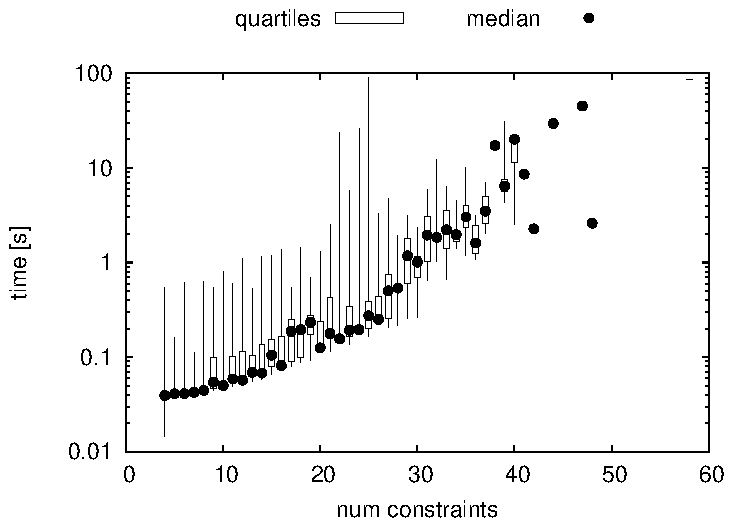
\includegraphics[width=8.5cm]{figures/plot_latte.pdf} \\
\caption{LattE benchmarks}
\label{fig:bench_latte}
\end{figure}
\fi

\section{Implementation and experiments}
\label{sec:impl}

We implemented an interpreter for the language based on the
probabilistic polyhedra powerset domain. The manipulations of
polyhedra are done using the PPL \cite{parma}. Size calculations are
done using the LattE \cite{latte}. LattE is also
used for the integer linear programming problem involved in the
abstract forget operation. The interpreter itself is written in OCaml.
We conducted several experiments on a Mac Pro with two 2.26 GHz
quad-core Xeon processors using 16 GB of RAM and running OS X v10.6.7.
While many of the abstract operations distribute over the set of
probabilistic polyhedra and thus could be parallelized, our
implementation is currently single-threaded.

\fref{fig:plots_bday}(a) illustrates the result of running the query
given in Example~\ref{ex:bday} (Section~\ref{sec:overview}) using our
implementation and one using Probabilistic
Scheme~\cite{radul07probscheme}, which is capable of sound probability
estimation after partial enumeration.  Each $\times$ plots
prob-scheme's maximum probability value (the y axis)---that is, the
probability it assigns to the most likely secret state---when given a
varying amount of time for sampling (the x axis).  We can see the
precision improves steadily until it reaches the exact value of 1/259
at around 17 seconds. Each $+$ plots our implementation's maximum
probability value when given an increasing number of probabilistic
polyhedra; with a polyhedral bound of 2 (or more), we obtain the exact
value in less than 3 seconds. The timing measurements are taken to be
the medians of 12 runs. The advantage of our approach is more evident
in \fref{fig:plots_bday}(b) where we use the same program but allow
$\var{byear}$ to span 1910 to 2010 rather than 1956 to 1992. In this
case prob-scheme makes little progress even after a minute, and
eventually runs out of memory.  Our approach, however, is unaffected
by this larger state space and produces the exact maximum belief in
around 3 seconds when using only 2 probabilistic polyhedra.

\ifacita

\fref{fig:plots_bday}(c) shows the result of assessing the special
query (Example~\ref{ex:specyear}) with initial belief matching that
following the first birthday query.  Each point is the number of
polyhedra allowed.  The result shows that more complex queries, ones
with many disjunctions, slow our approach and reduce the precision of
the maximum probability. The example requires 36 polyhedra for exact
calculations though as little as 3 produce probabilities near
exact. Note that the precision does not increase monotonically with
the number of polyhedra---in some cases more polyhedra leads to a less
precise result.  We conjecture that the occasional worsening of the
precision with increase in the number of allowable polyhedra is due to
an overly simple means of deciding which polyhedra to merge when
performing abstract simplification, a conjecture we plan to
investigate.

\else
\fref{fig:plots_bday}(c) shows the result of our implementation
assessing the special query (Example~\ref{ex:specyear}) with initial
belief matching that following the first birthday query.  Each plotted
point is the number of polyhedra allowed.  The result demonstrates
that more complex queries, specifically ones with many disjunctions in
their conditionals, not only slow our approach, but also reduce the
precision of the maximum probability value. The example requires 36
polyhedra for exact calculations though as little as 3 produce
probabilities near exact. Note that the precision does not increase
monotonically with the number of polyhedra---in some cases more
polyhedra leads to a less precise result.  We conjecture
that the occasional worsening of the precision with increase in the
number of allowable polyhedra is due to an overly simple means of
deciding which polyhedra to merge when performing abstract
simplification; we plan to investigate this issue in future work.
\fi

\iffull

Table~\ref{fig:bench_table} tabulates details for the example programs
along three other queries we developed based on advertising scenarios;
these queries are described in the Appendix~\ref{appendix:queries}. In
each box is the wall clock time for processing (median of 12 runs),
the running time's semi-interquartile range (SIQR), the number of
outliers, which are defined to be the points $ 3\times\text{SIQR} $
below the first quartile or above the third, and the max belief
computed (smaller being more accurate).  Obvious trends are that
running time goes up and max belief goes down as the number of
polyhedra increase, by and large.  There are exceptions to running
time trend, and most are close to the SIQR and so possibly not
statistically significant. The most striking exception is the running
time for poly-size 9 of the ``pizza'' query.  This extreme outlier is
due to a single invocation of LattE on the largest set of constraints
among all the benchmarks performed in the table. We have no good
explanation of how this complex polyhedron arose. \pxm{the previous
  was incorrect, we do know why the outlier exists, fixed.} The only
exceptions to monotonic decrease in max belief are the ``special
queries'', as already discussed.  \mwh{I observe that these are the
  only queries that employ probabilistic choice; any possibility this
  is correlated with the behavior?} \pxm{This might indirectly be the
  cause as it is the only example in which the postbelief is not a
  normalized restriction of the prebelief but I'm not sure how to
  better argue this Mike's hypothesis.}

Investigating the running time results further, we discovered that for
nearly all benchmarks, 95\% or more of the running time is spent in
the LattE counting tool.  The LattE tool exhibits super-exponential
running time in terms of the number of constraints (see
\fref{fig:bench_latte}) over the polyhedra that occur when evaluating
the various queries in Table~\ref{fig:bench_table}. As such, overall
running time is susceptible to the complexity of the polyhedra
involved, even when they are few in number. The merging operation,
while used to keep the number of probabilistic polyhedra below the
required bound, also tends to produce more complex polyhedra. These
observations suggest a great deal of performance improvement can be
gained by simplifying the polyhedra if they become too complex.

\fi

% LocalWords:  bday specyear bigmac


\section{Discussion}
\label{sec:future-work}

This section considers the some of the tradeoffs, challenges, design
alternatives, and possibilities for future work on knowledge-based
security policies and probabilistic polyhedra.

\subsection{Knowledge-based policies}

Employing knowledge-based policies successfully requires maintaining a
reasonable estimate of queriers' beliefs.  Two difficulties that arise
in doing so are (1) establishing the initial belief, and (2)
accounting for collusion among queriers.  Here we discuss
these two issues, and suggest further applications of knowledge-based
policies.

\paragraph*{Initial belief.}

For $P_1$ to enforce a knowledge-based policy on queries by $P_2$
requires that $P_1$ estimate $P_2$'s belief about the possible
valuations of $P_1$'s secret data.  When $P_2$ has no particular
knowledge of $P_1$'s secrets, statistical demographic data can be
used; e.g., the US Census and other public sources could be used for
personal information. When $P_2$ might have inside knowledge, $P_1$
must expend more effort to account for it.  For example, in a military
setting, estimating a coalition partner's estimate of one's resources
could be derived from shared information, and from the likelihood of
$P_2$ having acquired illicit information.  
Our benchmarks largely considered personal, private information, e.g.,
gender, age, level of education, etc.  This information can be drawn
from public sources (e.g., Facebook
demographics~\cite{facebook-demographics}).  However, the
distributions we experimented with were oversimplifications of the
actual, reported distributions: they were largely simple, uniform
distributions.  At present, the syntax of our query language
itself only allows specification of a single distribution. 
% Our
% abstraction has the benefit, however, of an approximate
% representation, which can be taken advantage of to easy the burden
% initial belief specification. A representation that attributes maximal
% probability of $ 1 $ to every state is technically sound (though
% not very useful). 
Of course, we could permit users to more directly specify
distributions of interest in a separate syntax.  A more interesting
alternative is to define the initial distribution using a
probabilistic program employing conditioning based on observations,
using the same mechanisms already developed to determining whether to
answer queries.  This is done in languages like IBAL~\cite{pfeffer07ibal} and
Fun~\cite{borgstrom11measure} and could be adapted to our setting.

% Machine learning techniques could be useful for our purposes
% here. Large bodies of work in ML deals with constructing models of
% probability distributions from samples, purported to come from said
% distributions. Recent work \cite{gordon13model} explores how to
% perform model learning using probabilistic language techniques. An
% interesting capability of this work is ability to specify models as
% programs, perform learning of the model given samples, and ascertain
% the model's imprecision via uncertainty in its parameters. Though the
% representations of distributions used there are different than the
% ones we use here, the same techniques could be applied here to learn
% an initial belief as a model from publicly visible samples.

If the initial belief estimate is (very) inaccurate, then $P_1$ risks
releasing information to $P_2$ contrary to his intended policy.  To
``hedge his bets'' against this possibility, he might choose to
maintain a set of possible beliefs $\Delta$, rather than a single
belief $\delta$, and only release if the threshold was satisfied for
every $\delta \in \Delta$.  We return to this idea in
Section~\ref{sec:diffpriv}. In some sense we already do maintain
multiple beliefs, as our implementation models/abstracts powersets of
probabilistic polyhedra, rather than single polyhedra, for performance
reasons.  We leave to future work the exploration of the practical
implementation of this idea.

\paragraph*{Collusion.}

Assuming that $P$ maintains separate beliefs and thresholds for
distinct queriers $Q_1$ and $Q_2$, the possibility of collusion
arises.  Following our motivating example in the Introduction, $P$'s
privacy would be thwarted if he shared only his birth day with $Q_1$
and only his birth year with $Q_2$ but then $Q_1$ and $Q_2$ shared
their information. This problem is not unique to our work; the same
problem would arise if $P$ used an access control policy to protect
birth day and birth year in the same way --- the policy will be
thwarted if $Q_1$ and $Q_2$ pool their information.

A simple approach to preventing this would be to model adversary
knowledge globally, effectively assuming that all queriers share their
query results; doing so would prevent either $Q_1$'s or $Q_2$'s query
(whichever was last). This approach is akin to having a global privacy
budget in differential privacy (see Section~\ref{sec:diffpriv}) or a
single, global access control policy and would obviously harm utility.
Moreover, the confidence of an agent can actually decrease as a result
of observing query outputs. This can occur when the agent is initially
confident in something that is not true, or as a result of improbable
outputs of probabilistic queries (like Example~\ref{ex:specyear}),
even when the agent is not mistakenly confident. Due to this
non-monotonicity in knowledge, if agents purported to be colluding are
in fact not colluding then a global belief might under-approximate a
non-colluding agent's true level of knowledge. \pxm{Second part of
  this para has changed.}

One possible compromise would be to consider both the potential of
collusion and non-collusion by tracking a global belief \emph{and} a
set of individual beliefs. When considering a query, a rejection would
be issued if either belief fails the policy check.

It is important to note that despite the possibility of a decreased
certainty due to queries, rational adversaries, interested in
maximizing their chances of guessing the secret value, will take all
outputs into account, even unlikely outcomes of probabilistic
queries. Though they might be detrimental to certainty, in
expectation, all queries increase chances of guessing the secret
correctly. This point is discussed further in the section on Accuracy,
Uncertainty, and Misinformation of
\cite{clarkson09quantifying}. \pxm{para changed}

\paragraph*{Further applications}

We have used the goal of decentralizing social networking applications
as a motivator for our technique.  But knowledge-based policies have
other applications as well.  Here are four examples.  

The first application is \emph{secure multiparty computation}
(SMC)~\cite{Yao86}.  Such computations allow a set of mutually
distrusting parties to compute a function~$f$ of their private inputs
while revealing nothing about their inputs beyond what is implied by
the result.  Depending on~$f$, however, the result itself may reveal
more information than parties are comfortable with.  Knowledge-based
policies can generalized to this setting: each party $X$ can assess
whether the other parties $Y_i$ could have secret values such that
$f$'s result would exceed a knowledge threshold about $X$'s secret.
We have explored two methods for implementing the generalized
knowledge threshold check; details are elsewhere~\cite{mardziel12smc}.

Another application is to protecting user browsing history.  With the
advent of ``do not track'' guidelines that forbid storing cookies to
track users' browsing habits across sites~\cite{dnt}, service
providers have turned to \emph{fingerprinting}, which aims to identify
a user based on available browser
characteristics~\cite{boda11fingerprint}.  We can protect these
attributes with knowledge-based policies, and enforce them by
analyzing the javascript code on browsed pages.  The flexibility of
knowledge-based policies is useful: with access control we would have
to choose, in advance, which attributes to reveal, but with
knowledge-based policies we can set a threshold on the entire tuple of
the most sensitive attributes and a web page can have access to
whatever (legal) subset of information it likes, for a better user
experience.

A third application is to protect sensing capabilities.  In
particular, we can treat sensor readings as samples from a random
process parameterized by confidential characteristics of the sensor.
Each reading provides information about these parameters, in addition
to information from the reading itself.  For example, suppose we want
to share mobility traces for traffic planning, but want to protect
individuals' privacy.  We can view each trace as a series of samples
from a random process that determines the individual's location based
on periodic factors, like previous location, time of day, day of week,
etc.~\cite{shokri11quantifying}.  We can define the sampling function in our simple
language, involving probabilistic choices over the hidden parameters.
Belief tracking can be used to narrow down the set of possible
parameters to the model that could have produced the observed traces;
if the observer's certainty about these parameters exceeds the
threshold, then the trace elements are not revealed.  Note that trace
obfuscation techniques are easily accounted for---they can simply be
composed with the sampling function and reasoned about together.

Finally, we observe that we can simply track the \emph{amount} of
released information due to an interaction as a degenerate case of
enforcing knowledge-based policies.  In particular, we can set the
pre-belief over some sensitive information to be the uniform
distribution, and set the threshold to be 1.  In this case, we will
always answer any query, and at any time we can compute the entropy of
the current belief estimate to calculate the (maximum) number of bits
leaked.  This information may be used to evaluate the susceptibility
to attack by gauging the confidence an attacker might have in their
belief about secret information.  It can be used to gauge what aspects
of secret information were of interest to the attacker, giving hints
to as their motive, or maybe even differentiating an honest querier
from a malicious one.  Tracking information in this manner is less
expensive than enforcing threshold policies directly, since not all
possible outputs need to be considered, and carries no risk of a
mis-estimate of the pre-belief: the number of reported leaked bits
will be conservatively high.

\subsection{Improving the Performance of Probabilistic Polyhedra}

While the performance of probabilistic polyhedra compares favorably to
alternative approaches, it can nevertheless be improved; this will be
important for applying it to the deployment scenarios listed above.  Here we
present several ideas for improving the implementation that we hope to
explore in future work.

\paragraph*{Handling nominal values.}  

Our probabilistic domains are based on polyhedra, octagons, and
intervals, which are best for analyzing programs with \emph{numeric}
variables, that contain linear conditionals. Most of the variables in
the benchmark programs were of the numeric variety. However, some were
\emph{nominal}, e.g., the variable encoding a user's language in the
travel query, and these are unordered.  Some variables are nominal but
partially ordered, like education level in the pizza query.  While we
can encode nominal values as integers, they may be better handled via
other means, perhaps even via na\"ive enumeration. Handling of large
quantities of nominal values could be performed symbolically using
some of the tools used by other probabilistic languages:
\cite{claret12bayesian}, graphical models \cite{milch05blog}, or
factor graphs \cite{borgstrom11measure, pfeffer07ibal}. Ideally
abstract domains like used in our system and ones better suited for
nominal values, could be integrated (i.e. via reduced product
\cite{cousot79systematic}) to effectively process programs that
contain both types of variables.

\paragraph*{Region splitting.}

As the performance experiments in the previous section show, intervals
can be far more efficient than polyhedra.  While a single interval may
be more imprecise than a single polyhedron, an interesting idea is
consider \emph{splitting} a polyhedron into many intervals, aiming for
the best of both worlds.  The simplest means of implementing this idea
is to modify the handling of the $ \suniformname $ statement for the
powerset domains to result not in one, but several intervals. Though a
single interval is sufficient to exactly represent distributions
produced by $ \suniformname $, it would be insufficient if, later, the
program introduces relations not representable by intervals. 

The challenge is to find the right tradeoff---increasing the number of
intervals will slowly degrade performance and may hurt precision if we
use an unfortunate merging order at join points, as seen in
Figure~\ref{fig:random_box}.  Heuristically picking the right merge
order is a known challenge in abstract interpretation-based analyses.

\paragraph*{Querier belief tracking.} 

Recall a vital property of our knowledge-based policy enforcement is
\emph{simulatability}: the adversary has (or is allowed to have) all
the information necessary to decide the policy that governs its
access, without interacting with the data owner. As such, the
computation of policy enforcement could, in theory, by done by the
querier.  Naturally, they should not be trusted in this regard
completely.  One general direction is to imagine the querier
performing the entire computation, and providing proof of the outcome,
via something like proof-carrying
code~\cite{necula97pcc}. Alternatively, the querier could provide
hints to the data owner to improve the speed of his computation.  For
example, the querier could determine the optimal choices for merge
order, and send a digest of these choices.

\section{Related work} \label{sec:related}
We consider four areas of work related to ours: systems aimed at
protecting access to users' private data; methods for quantifying
information flow from general-purpose programs; methods for
privacy-preserving computation, most notably \emph{differential
  privacy}; and finally approaches to performing general-purpose
probabilistic computation.

\subsection{Privacy enhancing network services}
Several recent proposals have considered alternative service
architectures for better ensuring the privacy of individual
participants.  These systems tend to enforce access control policies.
%
For example, PrPl~\cite{prpl} is a decentralized social networking
infrastructure aimed to permit participants to participate in social
networking without losing ownership of their data.  The system uses
\emph{Personal-Cloud Butler} services to store data and enforce access
control policies.  Persona~\cite{persona} uses a centralized
Facebook-style service, but users can store personal data on
distributed storage servers that use attribute-based encryption.
Access to data is granted to those parties who have the necessary
attribute keys.  XBook~\cite{xbook} mediates social network data
accesses by third-party application extensions.  Privad~\cite{privad}
is a privacy-preserving advertising platform that, like our running
examples, runs the ad selection algorithm over the user's data on the
user's platform.  Privad \emph{presumes} that outputs of ad selection
reveal little about the inputs.

Knowledge-based security policies generalize access control policies:
if we maintain a belief estimate for each principal $P$, then the
equivalent of granting $P$ access to data $d$ is to just set $P$'s
knowledge threshold for $d$ to 1; for principals $R$ who should not
have access, the threshold for $d$ is 0.  Knowledge-based policies
afford greater flexibility by allowing \emph{partial} access, i.e.,
when a threshold less than 1.  Moreover, as mentioned in the
introduction, we can set a policy on multiple data items, and thus
grant more access to one item than another (e.g., birth day and/or
year) as long as knowledge of the aggregate is controlled.

\subsection{Quantified information flow}
Others have considered how an adversary's knowledge of private data
might be informed by a program's output.  Clark, Hunt, and
Malacaria~\cite{clark2005QIF} define a static analysis that bounds the
secret information a straight-line program can leak in terms of
equivalence relations between the inputs and outputs.  Backes et
al.~\cite{backes09automatic} automate the synthesis of such
equivalence relations and quantify leakage by computing the exact size
of equivalence classes.  K\"opf and
Rybalchenko~\cite{kopf:rybalchenko} extend this approach, improving
its scalability by using sampling to identify equivalence classes and
using under- and over-approximation to obtain bounds on their size.
% \sbmcomment{Here we imply that the size of these blocks are important,
% but then Boris said that it is only the number of blocks that is of interest.
% Could we clarify this?} \mwh{They worry about class sizes to compute
% shannon entropy.  It's mentioned here because we care about sizes
% too.  I think we can just leave it given clarifications I make below.}
Mu and Clark~\cite{Mu:2009:inverval-qif} present a similar analysis
that uses over-approximation only.  In all cases, the inferred
equivalence classes can be used to compute entropy-based metrics of
information leakage.

We differ from this work in two main ways.  First, we implement a
different security criterion.  The most closely related metric is
\emph{conditional vulnerability} $V$ as proposed by
Smith~\cite{smith09foundations}, which can be defined using our
notation as follows:%\footnote{Smith actually proposes \emph{min
%    entropy}, which is $-\mathit{log}\;V$.}
\begin{definition}
\label{def:vul-threshold}
Let $\delta' = \eval{S}{\delta}$, where $\delta$ is the model of the
querier's initial belief.
%, and let $\overline{\delta_X} \defeq
%\normal{\project{\delta}{X}}$.

Then query $S$ is \emph{vulnerability threshold secure} iff for
%$$V = \sum_{\sigma_L \in
%  \nzset{\delta'_L}}\; \overline{\delta'_L}(\sigma_L) \cdot \max_{\sigma_H \in \states_H}\;
%  \overline{(\dcond{\delta'}{\sigma_L})_H}(\sigma_H)$$
$$V = \sum_{\sigma_L \in \support{\project{\delta'}{L}}}\;
  (\project{\delta'}{L})(\sigma_L) \cdot \max_{\sigma_H \in \states_H}\;
  (\project{\drevise{\delta'}{\sigma_L}}{H})(\sigma_H)$$
  we have $V \leq t$ for some threshold $t$.
\end{definition}
% $Pr[H=h] = (\project{\delta}{H})(h)$
% $Pr[H=h|L=l] = (\project{\dcond{\pevalp{S}{\delta}}{(L=l)}}{H})(h)$
% $Pr[L=l] = \dcond{\pevalp{S}{\delta}}{(L=l)}$
The above definition is an \emph{expectation} over all possible
outputs $\sigma_L$, so unlikely outputs have less influence.  Our
notion of threshold security (Definition~\ref{def:threshold}), in
contrast, is equivalent to a bound on the following quantity:
$$V^* = \max_{\sigma_L \in \support{\project{\delta'}{L}}}\;
\max_{\sigma_H \in \states_H}\;
(\project{\drevise{\delta'}{\sigma_L}}{H})(\sigma_H)$$

This notion of security is strictly stronger as it considers each
output individually: if \emph{any} output, however unlikely, would
increase knowledge beyond the threshold, the query would be rejected.
For example, recall the query from Example~\ref{ex:bday} where the
secret data $\var{bday}$ is (assumed by the querier to be) uniformly
distributed; call this query $S_1$.  According to
Definition~\ref{def:vul-threshold}, the minimum acceptable threshold
for which the query would be considered safe is $ V = \frac{7}{365} *
\frac{1}{7} + \frac{358}{365} * \frac{1}{358} = 2/365 \approx 0.005$,
whereas according to Definition~\ref{def:threshold}, the minimum
threshold is $ V^* = 1/7 \approx 0.143$.

The idea of strengthening of an entropy measure by eliminating the
expectation has been briefly considered by K{\"o}pf and Basin
\cite{koepfbasin07}. In their work this measure is proposed as a
stronger alternative, a choice ultimately dependent on the
application. In our case, however, the worst-case measure is
absolutely necessary in order to prevent the leakage of information
when rejecting a query.

The other distinguishing feature of our approach is that we keep an on-line model of
adversary knowledge according to prior, actual query results. Once a
query is answered, the alternative possible outputs of this query no
longer matter. To see the benefit of this
query-by-query approach, consider performing query $S_1$ followed by a
query $S_2$ which uses the same code as $S_1$ (from Example~\ref{ex:bday}) but has
$\var{today} = 265$.  With our system and $\var{bday} = 270$ the
answer to $S_1$ is $\sfalse$ and with the revised belief the query
$S_2$ will be accepted as below threshold $t_d = 0.2$.  If instead we
had to model this pair of queries statically they would be rejected
because (under the assumption of uniformity) the pair of outputs
$\strue$,$\strue$ is possible and implies $\var{bday} \in \{ 265, 266
\}$ which would require $t_d \geq 0.5$.  Our approach also inherits
from the belief-based approach the ability to model a querier who is
misinformed or incorrect, which can arise following the result of a
probabilistic query or because of a change to the secret data between
queries~\cite{clarkson09quantifying}.
% Probabilistic queries are not
% handled by the previously-described existing work that statically
% computes conditional min-entropy.  
We note these advantages come at the cost
of maintaining on-line belief models.

Our proposed abstract domains are useful beyond the application of
belief-based threshold security; e.g., they could be used to model
uncertainty off-line (as in the above work) rather than beliefs
on-line, with the advantage that they are not limited to uniform
distributions (as required
by~\cite{backes09automatic,kopf:rybalchenko}).

McCamant and Ernst's \flowcheck{} tool~\cite{McCamantE2008} measures
the information released by a particular execution.  However, it
measures information release in terms of \emph{channel capacity},
rather than remaining uncertainty which is more appropriate for our
setting.  For example, \flowcheck{} would report a query that tries to
guess a user's birthday leaks one bit regardless of whether the guess
was successful, whereas the belief-based model (and the other models
mentioned above) would consider a failing guess to convey very little
information (much less than a bit), and a successful guess conveying
quite a lot (much more than a bit).  

\subsection{Differential privacy}
\label{sec:diffpriv}

A recent thread of research has aimed to enforce the privacy of
database queries.  Most notably, Dwork and colleagues have proposed
\emph{differential privacy}~\cite{diffpriv}: a differentially private
query $Q$ over a database of individuals' records is a randomized
function that produces roughly the same answer whether a particular
individual's data is in the database or not.  An appealing feature of
this definition is that the querier's knowledge is not considered
directly; rather, we are merely assured that $Q$'s answer will not
differ by much whether a particular individual is in the database or
not. On the other hand, differentially private databases require that
individuals trust the database curator, a situation we would prefer to
avoid, as motivated in the introduction.

We can compare differential privacy to our notion of threshold
security by recasting the differential privacy definition into the
form of an \emph{adversarial privacy} definition, which was formulated
by Rastogi and Suciu to compare their own privacy definition on
databases to differential privacy~\cite{rastogi09relationship}.
Rastogi and Suciu's definition is in terms of the presence or
absence of a record in a database, whereas our notion is defined on
secret states over variables in $H$.  To bridge this gap suppose that,
without loss of generality, variables $x \in H$ range over $\{ 0, 1
\}$, and we say a variable $x$ is ``in a state'' $\sigma$ when
$\sigma(x) = 1$. (We can always encode an integer $i$ as a sequence of
bits.)  Define $\delta(\{x_1,...,x_n\})$ to be the probability of all
states $\sigma$ such that $\sigma(x_i) = 1$ for all $1 \leq i \leq n$;
i.e.,
$$\delta(\{x_1,...,x_n\}) \defeq 
\sum_{\sigma \mid
  \sigma(x_1) = 1 \wedge ... \wedge \sigma(x_n) = 1} \delta(\sigma) 
$$
Then we can state adversarial privacy as follows.

\begin{definition}[Adversarial Privacy]
\label{def:adv-privacy}
Given a query statement $\stmt$, let $O \subseteq \states_{L\cup H}$
be the set of all possible output states of $\stmt$ (over some set of
secret variables $H$ and public variables $L$), and $\Delta_H \subseteq
\dists_H$ be a set of distributions over secret states.
%
We say that program $\stmt$ is $\varepsilon$-\emph{adversarially
  private} w.r.t. $\Delta_H$ iff for all adversary beliefs $\delta_H
\in \Delta_H$, all secret variables $x \in H$, and all possible
outputs $\sigma_o \in O$, that $\delta_H(\{x\}) \leq e^{\varepsilon}\,
\delta'_H(\{x\})$.  Here, $\delta'_H =
\project{(\evalp{\stmt}{(\delta_H \times \dot{\sigma}_L)}) |
  \sigma_o}{H}$; that is, it is the revised adversary belief after
seeing that public output state of $\stmt$ is $\sigma_o$.
\end{definition}

This definition says that query $\stmt$ is acceptable when the output
of $S$ increases only by a small multiplicative factor an adversary's
certainty that some variable $x$ is in the secret input state, for all
adversaries whose prebeliefs are characterized by $\Delta_H$.  Rastogi
and Suciu show that defining $\Delta_H$ to be the class of
\emph{planar, total sub-modular} (or $PTLM$) distributions renders an
adversarial privacy definition equivalent to differential privacy.
Among other conditions, $PTLM$ distributions require fixed-sized
databases (which comes by construction in our setting), and require
the probability of one tuple's presence to not be positively
correlated with another's.  We can transfer this latter condition to
our setting by requiring that for all $\delta \in \Delta_H$, and all
$x_1,x_2 \in H$, we have $\delta(\{x_1\}) \delta(\{x_2\}) \leq
\delta(\{x_1,x_2\})$.

Comparing Definition~\ref{def:adv-privacy} to
Definition~\ref{def:threshold} we can see that the former makes a
\emph{relative} assertion about the increased certainty of any one of
a \emph{set} of possible adversarial beliefs, while the latter makes
an \emph{absolute} assertion about the certainty of a \emph{single}
adversarial belief.  The absolute threshold of our definition is
appealing, as is the more flexible prebelief, which allows positive
correlations among state variables.  On the other hand, our definition
assumes we have correctly modeled the adversary's belief.  While this
is possible in some cases, e.g., when demographic information is
available, differential privacy is appealing in that it is robust a
much larger number of adversaries, i.e., all those whose prebeliefs
are in $PTLM$.

Unfortunately, this strong privacy guarantee seems to come at strong
cost to utility.  For example, deterministic queries are effectively
precluded, eliminating some possibly useful applications.  
For the application of social
networks, Machanavajjhala et al.~\cite{machanavajjhala11personal} have
shown that good private social recommendations are feasible only for a
small subset of the users in the social network or for a lenient
setting of privacy parameters.  We can see the utility loss in our
motivating scenario as well.  Consider the birthday query from
Example~\ref{ex:bday}.  Bob's birthday being/not being in the query
range influences the output of the query only by 1 (assuming yes/no is
1/0). One could add an appropriate amount of (Laplacian) noise to the
query answer to hide what the true answer was and make the query
differentially private. However, this noise would be so large compared
to the original range $\{0,1\}$ that the query becomes essentially
useless---the user would be receiving a birthday announcement most
days.\footnote{By our calculations, with privacy parameter $\varepsilon =
  0.1$ recommended by Dwork~\cite{diffpriv}, the probability the query
  returns the correct result is approximately $0.5249$.}  

By contrast, our approach permits answering (deterministic or
randomized) queries exactly if the release of information is below the
threshold.  Moreover, by tracking beliefs between queries, there is no
artificial limit on the number of queries since we can track the
released information exactly.  Differential privacy imposes an artificial
limit on the number of queries because the post-query, revised beliefs
of the adversary are not computed.  Rather, each query conservatively
adds up to $\varepsilon$ to an adversary's certainty about a tuple,
and since the precise release is not computed, we must assume the
worst.  Eventually, performing further queries will pose too great of a risk.

As mentioned in the previous section, we could gain some of the
privacy advantages of differential privacy by modeling a (larger) set
of beliefs rather than a single one.  Our abstractions $\ppolys$ and
$\ppowers$ already model sets of distributions, rather than a single
distribution, so it remains interesting future work to exploit this
representation toward increasing privacy.

\subsection{Probabilistic programming}
The core of our methodology relies on probabilistic computation. A
variety of tools exist for specifying random processes as computer
programs and performing inference on them.

Implementations based on partial sampling \cite{goodman08church,
  park08sampling} or full enumeration \cite{radul07probscheme} of the
state space are unsuitable in our setting. Such tools are either too
inefficient or too imprecise. Works based on smarter representations
of probability distributions are promising alternatives. Projects
based on algebraic decision diagrams \cite{claret12bayesian},
graphical models \cite{milch05blog}, and factor graphs
\cite{borgstrom11measure, pfeffer07ibal} translate programs into
convenient structures and take advantage of efficient algorithms for
their manipulation or inference.

Our implementation for probabilistic computation and inference differs
from existing works in two main ways. Firstly, we are capable of
approximation and hence can trade off precision for performance, while
maintaining soundness in terms of a strong security policy. The second
difference is the nature of our representation of probability
distributions. Our work is based on numerical abstractions: intervals,
octagons, and polyhedra. These abstractions are especially well suited
for analysis of imperative programs with numeric variables and linear
conditionals. Other probabilistic languages
might serve as better choices when nominal, rather than numeric,
variables are used in queries. The comparative study of the power and effectiveness
of various representations in probabilistic computation is a topic of
our ongoing research.

We are not the first to propose probabilistic abstract
interpretation. Monniaux~\cite{Monniaux_these} gives an abstract
interpretation for probabilistic programs based on over-approximating
probabilities of points. Di Pierro describes abstract interpretation
for probabilistic lambda calculus
\cite{dipierro05probabilistic}. Smith~\cite{smith08probabilistic}
describes probabilistic abstract interpretation for verification of
quantitative program properties. Cousot~\cite{cousot12probabilistic}
unifies these and other probabilistic program analysis tools. However,
these do not deal with sound distribution conditioning, the unique
element of our approach, which is crucial for belief-based information
flow analysis.

% Following the flow of our example from Section~\ref{sec:overview},
% when advertiser $X$ submits Example~\ref{ex:specyear}, a result of
% $\strue$ will lead $X$ to believe that $1980$ (Bob's actual birthday)
% is a less likely birth year ($1/11814 \times 268 = 0.023$) than he
% previously thought ($1/37 = 0.027$).  Suppose we are using $X$'s
% modeled belief (call it $\delta_X$) to also model $Y$'s knowledge,
% where $Y$ would otherwise give $1980$ has probability $1/37$ (i.e., if
% we were modeling $Y$'s knowledge separately as $\delta_Y$).  If Bob's
% threshold for his birth year is $t_{yr} = 0.03$, then under $\delta_X$
% a query \mwh{need to choose a query in which we'd reject under
%   $\delta_Y$ but not under $\delta_X$}.

% One way to address this problem is to allow only deterministic
% queries.  Then there is no misinformation.  Obviously doing this
% reduces the system's expressive power.  Another possibility is to
% force knowledge to be monotonic: if an accepted query Q would cause
% the posterior certainty to be reduced, we do not change the modeled
% belief, but leave it as is.  I haven't thought carefully about the
% ramifications of doing so, though.  I suspect the result is simply
% conservative, but I need to think harder about whether it's unsafe.

% So, in short, I think that DP has problems with collusion, but these
% problems are entirely in terms of utility, not performance or
% safety.  That is, DP, can have a global privacy budget and while
% using such a mechanism will severely limit utility, it will not harm
% privacy.  In our case, we could model many belief sets to avoid the
% safety problems, but at an enormous performance cost, and at some
% cost to utility (the same flavor as DP, i.e., if principals were not
% really colluding).  Or, we could ignore the possibility of collusion
% to regain performance and utility, but impose some risk on safety.

% But there is a key difference to your approach: [25,26] use *conditional* min-entropy as a measure, which is (in some sense) the expected min-entropy over all possible choices of secrets. An iterative application (and summing conditional min-entropy, as suggested above) implicitly assumes that the secret is freshly chosen in each run. While this is a sound over-approximation of what the adversary may learn, its knowledge will never level off (as it may do in your approach). This is a clear advantage of the belief-based approach.

%%In any case, we believe there is much to be said for both approaches, and hope that this paper serves as another useful step on the path toward practical privacy-preserving computation.


%%For example, if a client
%%wants to determine what proportion of Facebook users are male, this
%%query will be permitted, as the removal of a particular user's data
%%will not significantly affect the result.  However in the course of
%%computing this result, substantial access to individual user data is
%%required.   In the absence of a system for secure multi-party
%%computation \cite{fairplaymp}, the agent computing the result must
%%have full access to gender information for each user, so that the
%%number of male users and female users can be determined.  Such queries
%%would leak too much individual information.

%%Thus, it would appear that we need a trusted third party to execute
%5these queries.  However, in our approach one can use the probabilistic conditional
%%\textsf{pif} to permit certain types of data aggregation.  For our
%%Facebook gender example, an estimate of the proportion of users who
%%are male can be obtained by executing the query below.  We assume that
%%gender is encoded as a binary value, where 0 represents ``male.''

%%\[\spif{0.6}{output := gender}{output := not(gender)}\]

%% This gives the client imperfect information about each user, but this
%5information is still useful in aggregate. For 60\% of the queries, the
%%client will get the correct gender.  If all users are male, the client would
%%expect 60\% of the queries to return 0.  If all users are female, the client
%%would expect 40\% of the queries to return 0.  The percentage in between
%%correspond to varying percentages of male users, with the crossover point
%%being 50\%---if more than 50\% of the queries return 0, then there are likely
%%to be more males than females (where the likelihood depends on the number
%%of users that are sampled).

%%Second, our approach investigates a knowledge-based policy that succinctly captures the semantics of the information that has thus far been revealed to a querier via one or more queries. While differential privacy allows the queried entity to cumulatively track loss in privacy over one or more queries~\cite{PINQ-SIGMOD09}, it fails to consider semantic overlap between such queries $-$ thereby weakening the tightness of their estimates.


%% to pass the individual privacy
%%monitoring \sbmcomment{better term for this?} system described
%%here.



%% Recent advances have explored the notion of adversarial privacy~\cite{rastogi09relationship} to partially bridge this semantic gap by explicitly modeling the adversary's belief on the input dataset. In their setting privacy is defined by the closeness between the posterior and prior distribution on the likelihood of a tuple after seeing the output of query. Their approach is shown to offer tighter estimates by proving that adversarial privacy under a bounded belief model subsumes differential privacy. While their approach quantitatively estimates privacy loss wrt to the querier's belief (as against differential privacy that is agnostic to the querier's belief), they fail to capture the semantics of the information released via one or more queries. Further, similar to differential privacy, adversarial privacy is designed to operate on aggregate data from multiple individuals.

%%Differential privacy~\cite{diffpriv}: works on aggregate data, not on
%%individual data; fixed number of possible queries allowed until the
%%data must be destroyed (cannot even answer the same query twice).  By
%%contrast, our approach models semantic knowledge, so you can ask the
%%same question in different ways and still get an answer.

%%Also want to talk about Rastogi and Suciu's stuff.

%%Backes et al.~\cite{backes09automatic} model information leakage in a program as (the size of) an equivalence relationship between the set of input and output symbols. While their approach quantifies per-program entropy measures, they also fail to offer fine-grained (per query) semantically richer approach to track information release.

%%\mwh{More rambling below}

%%Diffpriv different in that they don't model belief explicitly, but they do have a privacy ``budget'' $\epsilon$.  In effect this is a counter of the amount of knowledge they are willing to let an attacker gain.  While they are not required to model a belief explicitly, which is an advantage, they need to have the assumed level of knowledge in mind in order to set $\epsilon$.  A disadvantage of the indirect modeling of knowledge is that it is difficult to reason how much a query $q$ overlaps with a prior query $q'$.  As such, the default is to presume all queries reveal (equivalent) knowledge, and so there is a fixed number of queries a particular principal may pose.  Also, equally vulnerable to collusion as our approach.  I wonder: how does diffpriv handle changing values?  Work on declassification/anonymization: picks values to release in advance, so less flexibility for the querier.  In scenarios like SMC, this could be a showstopper.  But this is simpler to implement and resistant to collusion.  Could imagine combining pro-active anonymization with belief-based policies.

%%\mwh{Taken from introduction, to work in here}:


%%Returning exact results is in contrast to approaches like differential privacy~\cite{diffpriv}
%%that, while also limiting which queries may be performed, must add
%%noise to increase uncertainty, since knowledge is not modeled
%%directly.

%%\todo{Mention limitations somewhere: what about collusion?
%%  What if you get the belief models wrong?  How to deal with
%%  non-discrete data, or fixed-length loops?}

%%\mwh{Work the following into the discussion of differential privacy?}



%%\mwh{and more ...}

%%Differential privacy guarantees that privacy is preserved by ensuring
%%that sufficient data aggregation occurs.  

%%\sbmcomment{Would be good to make this more formal.  What are the equations
%%that yield the likely percentage of males and the confidence in this estimate?}



\section{Conclusion}
\label{sec:conc}

This paper has explored the idea of \emph{knowledge-based security
  policies}: given a query over some secret data, that query should
only be answered if doing so will not increase the querier's knowledge
above a fixed threshold.  We enforce knowledge-based policies by
explicitly tracking a model of a querier's belief about secret data,
represented as a probability distribution, and we deny any query that
could increase knowledge above the threshold.  Our denial criterion is
independent of the actual secret, so denial does not leak information.
We implement query analysis and belief tracking via abstract
interpretation using domains of \emph{powersets of probabilistic
polyhedra, octagons, and intervals}.
%
Compared to typical approaches to implementing belief revision, our
implementation using this domain is more efficient and scales better.

\vspace*{.1in}
\begin{small}
\paragraph*{Acknowledgments} The authors are
grateful to Jeff Foster, Nataliya Guts, the CSF'11 anonymous referees, and
especially Boris K\"opf for their helpful comments on
drafts of this paper.  

This research was sponsored by the U.S. Army
Research Laboratory and the U.K. Ministry of Defence and was
accomplished under Agreement Number W911NF-06-3-0001. The views and
conclusions contained in this document are those of the author(s) and
should not be interpreted as representing the official policies,
either expressed or implied, of the U.S. Army Research Laboratory, the
U.S. Government, the U.K. Ministry of Defence or the
U.K. Government. The U.S. and U.K. Governments are authorised to
reproduce and distribute reprints for Government purposes
notwithstanding any copyright notation hereon.  Support was also
provided by National Science Foundation grants 0905419 and
0910530.
\end{small}

\bibliographystyle{plain}
\balance
\bibliography{paper}

%\appendices
\appendix

%\vspace*{.1in}
%\section{Concrete probabilistic semantics}
%\label{appendix:concrete}
%
%Here we briefly explain the concrete probabilistic semantics given in
%Figure~\ref{fig-sem-nondet2-core}.  More details can be found in
%Clarkson et al.~\cite{clarkson09quantifying}.
%
%The semantics of $\sskip$ is straightforward: it is the identity on
%distributions.  The semantics of sequences $\sseq{\stmt_1}{\stmt_2}$
%is also straightforward: the distribution that results from executing
%$\stmt_1$ with $\delta$ is given as input to $\stmt_2$ to produce
%the result.
%
%The semantics of assignment is $\delta \bparen{x \ra \aexp}$, which is
%defined as follows: 
%$$ \delta \bparen{x \ra \aexp} \defeq \lambda \sigma \lsep \sum_{\tau \; | \; \tau
%  \bparen{x \ra \eeval{\aexp}{\tau}} = \sigma} \delta (\tau) $$ In
%words, the result of substituting an expression $\aexp$ for $x$ is a
%distribution where state $\sigma$ is given a probability that is the
%sum of the probabilities of all states $\tau$ that are equal to
%$\sigma$ when $x$ is mapped to the distribution on $\aexp$ in $\tau$.
%For implementation purposes, it will be useful to consider separately the
%case where assignment is invertible.
%
%When $x \ra \aexp$ is an invertible transformation, the formula for
%assignment can be simplified to the following, where $x \ra \aexp'$ is
%the inverse of $x \ra \aexp$.
%\[
%\delta \bparen{x \ra \aexp} \defeq \lambda \sigma \lsep \delta (\sigma\bparen{x \ra \eeval{\aexp'}{\sigma}})
%\]
%
%When $x \ra \aexp$ is not invertible, the original definition is
%equivalent to a projection followed by an assignment.  Let $V'
%= \fv{\delta} - \{x\}$ and let $\delta' = \project{\delta}{V'}$.
%Then we have the following for a non-invertible assignment.
%\[\delta \bparen{x \ra \aexp} \defeq \lambda \sigma \lsep \aif \sigma(x) = \eeval{E}{\sigma}\athen
%\delta'(\project{\sigma}{V'}) \aelse 0 \]
%We prove this definition by cases is
%equivalent to the original definition in the companion technical report~\cite{TR}.
%
%The semantics for conditionals makes use of two operators on
%distributions which we now define.  First, given distributions
%$\delta_1$ and $\delta_2$ we define the \emph{distribution sum} as
%follows:
%$$ \delta_1 + \delta_2 \defeq \lambda \sigma \lsep \delta_1(\sigma) +
%\delta_2(\sigma) $$ In words, the probability mass for a given state
%$\sigma$ of the summed distribution is just the sum of the masses from
%the input distributions for $\sigma$.  Second, given a distribution
%$\delta$ and a boolean expression $\bexp$, we define the
%\emph{distribution conditioned on $\bexp$} to be
%$$ \dcond{\delta}{\bexp} \defeq \lambda \sigma \lsep \aif \eeval{\bexp}{\sigma} \athen
%\delta(\sigma) \aelse 0 $$
%In short, the resulting distribution retains only the probability mass
%from $\delta$ for states $\sigma$ in which $\bexp$
%holds.
%
%With these two operators, the semantics of conditionals can be stated
%simply: the resulting distribution is the sum of the distributions of
%the two branches, where the first branch's distribution is conditioned
%on $\bexp$ being true, while the second branch's distribution is
%conditioned on $\bexp$ being false.
%
%The semantics for probabilistic conditionals like that of conditionals
%but makes use of \emph{distribution scaling}, which is defined as
%follows: given $\delta$ and some scalar $p$ in $[0,1]$, we have
%$$ p \cdot \delta \defeq \lambda \sigma \lsep p \cdot \delta(\sigma) $$
%In short, the probability ascribed to each state is just the
%probability ascribed to that state by $\delta$ but multiplied by $p$.
%For probabilistic conditionals, we sum the distributions of the two
%branches, scaling them according to the odds $q$ and $1 - q$.
%
%The semantics of a single iteration of a while loop is
%essentially that of $\sif{B}{S}{\sskip}$ and the semantics of the
%entire loop is the fixed point of a function that composes the
%distributions produced by each iteration.  That such a fixed point exists
%is proved by Clarkson et al.~\cite{clarkson09quantifying}.
%
%Finally, the semantics of $\suniform{x}{n_1}{n_2}$, introduced in
%Section~\ref{sec:absinterp} is given as
%$$
%\begin{array}{rcl}
%\pevalp{\suniform{x}{n_1}{n_2}}{\delta} & = &
%\paren{\project{\delta}{V - \set{x}}} \times \delta'
%\end{array}
%$$
%Where $ V $ is the set of variables of $ \delta $, and $ \delta' $ is
%defined as follows.
%$$ \delta ' = \lambda \sigma \lsep \aif n_1 \leq \sigma(x) \leq n_2 \athen
%\frac{1}{n_2-n_1+1} \aelse 0 $$
%
\vspace*{.1in}
\section{Example queries} \label{appendix:queries}

%rendering latex
$$ \ssecretk: $$
\begin{displaymath}{\small
\begin{array}{l}
  \sassign{country}{1}\; ;\\
  \sassign{birth\text{\_}year}{1983}\; ;\\
  \sassign{completed\text{\_}school\text{\_}type}{4}\; ;\\
  \sassign{language}{5}\\
\end{array}
}
\end{displaymath}
$$ \sbeliefk: $$
\begin{displaymath}{\small
\begin{array}{l}
  \suniform{country}{1}{200}\; ;\\
  \suniform{birth\text{\_}year}{1900}{2011}\; ;\\
  \suniform{language}{1}{50}\; ;\\
  \suniform{completed\text{\_}school\text{\_}type}{0}{5}\\
\end{array}
}
\end{displaymath}

$$ \squerydefk \; travel \; : \; \; \ra \; output$$
\begin{displaymath}{\small
\begin{array}{l}
  \sifk \; country \; = \; 1 \; \vee \; country \; = \; 3 \; \vee \; country \; = \; 8 \; \vee \; country \; = \; 10 \; \vee \; country \; = \; 18 \; \sthenk\\
  \;\;\;\sassign{main\text{\_}country}{1}\\
  \selsek\\
  \;\;\;\sassign{main\text{\_}country}{0}\; ;\\
  \sifk \; country \; = \; 169 \; \vee \; country \; = \; 197 \; \vee \; country \; = \; 194 \; \vee \; country \; = \; 170 \; \vee \; country \; = \; 206 \; \vee \; country \; = \; 183 \; \vee \; country \; = \; 188 \; \sthenk\\
  \;\;\;\sassign{island}{1}\\
  \selsek\\
  \;\;\;\sassign{island}{0}\; ;\\
  \sassign{age}{\ebinop{-}{2010}{birth\text{\_}year}}\; ;\\
  \sifk \; language \; = \; 1 \; \wedge \; main\text{\_}country \; = \; 1 \; \vee \; island \; = \; 1 \; \wedge \; age \; \geq \; 21 \; \wedge \; completed\text{\_}school\text{\_}type \; \geq \; 4 \; \sthenk\\
  \;\;\;\sassign{output}{1}\\
  \selsek\\
  \;\;\;\sassign{output}{0}\\
\end{array}
}
\end{displaymath}


$$ \squeryk \; travel \; : $$
\begin{displaymath}{\small
\begin{array}{l}
  \sskip\\
\end{array}
}
\end{displaymath}

no errors


We provide here the queries and prebeliefs we used for the experiments
in Section~\ref{sec:impl}. The queries are described as functions
from some set of inputs to some set of outputs. The exact syntax is as
follows.
$$
\begin{array}{l}
\squerydefk \; queryname \; in_1 \cdots in_n \ra out_1 \cdots out_m \; : \\
\;\; querybody \\
\end{array}
$$

Query definitions that follow sometimes include
pre-processing statements of the form:
$$ \psdefine{x}{exp} $$
Such statements result in any occurrence of a variable $ x $ being
replaced by the expression $exp$. This is used for convenience to
refer to common expressions without actually requiring the analysis to
track additional variables/dimensions.

To specify a query invocation we use the following syntax.
$$
\begin{array}{l}
\squeryk \; queryname \; : \\
\;\; in_1 \; := \; val_1; \\
\;\; \cdots \\
\;\; in_n \; := \; val_n
\end{array}
$$
Each experiment must also specify the values of the secrets being
queried, and the querier's prebelief.  Each specification is a merely
a program that sets the values of these variables.  For the actual
secret values this program begins with the declaration $ \ssecretk$;
the resulting state of executing program is taken to be the secret
state.  The program to set the prebelief begins $ \sbeliefk$ and has
the same format; note that this program will use $\spifk$ or
$\suniform{x}{n_1}{n_2}$ to give secrets different possible values
with different probabilities.  

We now give the content of the queries used in the experiments.

\subsection{Birthday}
For the small stateset size birthday experiments we used the
following secret and prebelief.
$$ \ssecretk: $$
\begin{displaymath}{\small
\begin{array}{l}
  \sassign{s\text{\_}bday}{270}\; ;\\
  \sassign{s\text{\_}byear}{1980}\\
\end{array}
}\end{displaymath}
$$ \sbeliefk: $$
\begin{displaymath}{\small
\begin{array}{l}
  \suniform{s\text{\_}bday}{0}{364}\; ;\\
  \suniform{s\text{\_}byear}{1956}{1992}\\
\end{array}
}\end{displaymath}

The two queries used were as follows.

$$ \squerydefk \; bday \; : \;c\text{\_}day \; \ra \; out$$
\begin{displaymath}{\small
\begin{array}{l}
  \sifk \; \ebinop{\wedge}{\ebinop{\geq}{s\text{\_}bday}{c\text{\_}day}}{\ebinop{>}{\ebinop{+}{c\text{\_}day}{7}}{s\text{\_}bday}} \; \sthenk\\
  \;\;\;\sassign{out}{1}\\
  \selsek\\
  \;\;\;\sassign{out}{0}\\
\end{array}
}\end{displaymath}

$$ \squerydefk \; spec \; : \;c\text{\_}year \; \ra \; out$$
\begin{displaymath}{\small
\begin{array}{l}
  \psdefine{age}{\ebinop{-}{c\text{\_}year}{s\text{\_}byear}}\\
  \sifk \; \lbinop{\vee}{\lbinop{\vee}{\lbinop{\vee}{\lbinop{\vee}{\lbinop{\vee}{\lbinop{\vee}{\lbinop{\vee}{\lbinop{\vee}{\lbinop{\vee}{\lreln{=}{age}{10}}{\lreln{=}{age}{20}}}{\lreln{=}{age}{30}}}{\lreln{=}{age}{40}}\\\;}{\lreln{=}{age}{50}}}{\lreln{=}{age}{60}}}{\lreln{=}{age}{70}}}{\lreln{=}{age}{80}}\\\;}{\lreln{=}{age}{90}}}{\lreln{=}{age}{100}}\; \sthenk\\
  \;\;\;\sassign{out}{1}\\
  \selsek\\
  \;\;\;\sassign{out}{0}\; ;\\
  \spifk\; 1/10 \; \sthenk\\
  \;\;\;\sassign{out}{1}\\
\end{array}
}
\end{displaymath}

The statistics described in comparison to the enumeration approach
(Section~\ref{sec:enum}) include the time spent processing this
initial setup as well as time processing one birthday
query. Figure~\ref{fig:bench_domains_bday_large} benchmarks two bday
queries followed by a spec year query.

\begin{itemize}
\item{} A single bday query alone.
$$ \squeryk \; bday \; : $$
\begin{displaymath}{\small
\begin{array}{l}
  \sassign{c\text{\_}day}{260}\\
\end{array}
}\end{displaymath}

\item{} Two bday queries followed by a spec query.
$$ \squeryk \; bday \; : $$
\begin{displaymath}{\small
\begin{array}{l}
  \sassign{c\text{\_}day}{260}\\
\end{array}
}\end{displaymath}
$$ \squeryk \; bday \; : $$
\begin{displaymath}{\small
\begin{array}{l}
  \sassign{c\text{\_}day}{261}\\
\end{array}
}\end{displaymath}
$$ \squeryk \; spec \; : $$
\begin{displaymath}{\small
\begin{array}{l}
  \sassign{c\text{\_}year}{2011}\\
\end{array}
}\end{displaymath}

\end{itemize}

\subsection{Birthday (large)}

For the larger statespace birthday example we used the following
secret and prebelief generators.
$$ \ssecretk: $$
\begin{displaymath}{\small
\begin{array}{l}
  \sassign{s\text{\_}bday}{270}\; ;\\
  \sassign{s\text{\_}byear}{1980}\\
\end{array}
}\end{displaymath}
$$ \sbeliefk: $$
\begin{displaymath}{\small
\begin{array}{l}
  \suniform{s\text{\_}bday}{0}{364}\; ;\\
  \suniform{s\text{\_}byear}{1910}{2010}\\
\end{array}
}\end{displaymath} The queries used were identical to the ones for the
smaller statespace birthday example. For our benchmarks we analyzed
the vulnerability of the pair of secrets $ s\text{\_}bday,
s\text{\_}byear $.

\subsection{Pizza}

The pizza example is slightly more complicated, especially in the
construction of the prebelief.  This example models a targeted
Facebook advertisement for a local pizza shop.  There are four
relevant secret values.  The level of school currently being attended
by the Facebook user is given by \verb|s_in_school_type|, which is an
integer ranging from 0 (not in school) to 6 (Ph.D. program).  Birth
year is as before and \verb|s_address_lat| and \verb|s_address_long|
give the latitude and longitude of the user's home address
(represented as decimal degrees scaled by a factor of $10^6$ and
converted to an integer).

The initial belief models the fact that each subsequent level of
education is less likely and also captures the correlation between
current educational level and age.  For example, a user is given an
approximately 0.05 chance of currently being an undergraduate in
college, and college attendees are assumed to be born no later than
1985 (whereas elementary school students may be born as late as 2002).

$$ \ssecretk: $$
\begin{displaymath}{\small
\begin{array}{l}
  \sassign{s\text{\_}in\text{\_}school\text{\_}type}{4}\; ;\\
  \sassign{s\text{\_}birth\text{\_}year}{1983}\; ;\\
  \sassign{s\text{\_}address\text{\_}lat}{39003178}\; ;\\
  \sassign{s\text{\_}address\text{\_}long}{-76958199}\\
\end{array}
}
\end{displaymath}
$$ \sbeliefk: $$
\begin{displaymath}{\small
\begin{array}{l}
  \spifk\; 4/24 \; \sthenk\\
  \;\;\;\suniform{s\text{\_}in\text{\_}school\text{\_}type}{1}{1}\; ;\\
  \;\;\;\suniform{s\text{\_}birth\text{\_}year}{1998}{2002}\\
  \selsek\\
  \;\;\;\spifk\; 3/19 \; \sthenk\\
  \;\;\;\;\;\;\suniform{s\text{\_}in\text{\_}school\text{\_}type}{2}{2}\; ;\\
  \;\;\;\;\;\;\suniform{s\text{\_}birth\text{\_}year}{1990}{1998}\\
  \;\;\;\selsek\\
  \;\;\;\;\;\;\spifk\; 2/15 \; \sthenk\\
  \;\;\;\;\;\;\;\;\;\suniform{s\text{\_}in\text{\_}school\text{\_}type}{3}{3}\; ;\\
  \;\;\;\;\;\;\;\;\;\suniform{s\text{\_}birth\text{\_}year}{1985}{1992}\\
  \;\;\;\;\;\;\selsek\\
  \;\;\;\;\;\;\;\;\;\spifk\; 1/12 \; \sthenk\\
  \;\;\;\;\;\;\;\;\;\;\;\;\suniform{s\text{\_}in\text{\_}school\text{\_}type}{4}{4}\; ;\\
  \;\;\;\;\;\;\;\;\;\;\;\;\suniform{s\text{\_}birth\text{\_}year}{1980}{1985}\\
  \;\;\;\;\;\;\;\;\;\selsek\\
  \;\;\;\;\;\;\;\;\;\;\;\;\suniform{s\text{\_}in\text{\_}school\text{\_}type}{0}{0}\; ;\\
  \;\;\;\;\;\;\;\;\;\;\;\;\suniform{s\text{\_}birth\text{\_}year}{1900}{1985}\; ;\\
  \suniform{s\text{\_}address\text{\_}lat}{38867884}{39103178}\; ;\\
  \suniform{s\text{\_}address\text{\_}long}{-77058199}{-76825926}\\
\end{array}
}
\end{displaymath}

The query itself targets the pizza advertisement at users who are
either in college or aged 18 to 28, while living close to the pizza
shop (within a square region that is 2.5 miles on each side and
centered on the pizza shop).  If this condition is satisfied, then the
query returns 1, indicating that the ad should be displayed.  The full
text of the query is given below.

$$ \squerydefk \; pizza \; : \; \; \ra \; out$$
\begin{displaymath}{\small
\begin{array}{l}
  \psdefine{age}{\ebinop{-}{2010}{s\text{\_}birth\text{\_}year}}\\
  \psdefine{lr\text{\_}lat}{38967884}\\
  \psdefine{ul\text{\_}lat}{39003178}\\
  \psdefine{lr\text{\_}long}{-76958199}\\
  \psdefine{ul\text{\_}long}{-76925926}\\
  \sifk \; \lreln{\geq}{s\text{\_}in\text{\_}school\text{\_}type}{4} \; \sthenk\\
  \;\;\;\sassign{in\text{\_}school}{1}\\
  \selsek\\
  \;\;\;\sassign{in\text{\_}school}{0}\; ;\\
  \sifk \; \lbinop{\wedge}{\lreln{\geq}{age}{18}}{\lreln{\leq}{age}{28}} \; \sthenk\\
  \;\;\;\sassign{age\text{\_}criteria}{1}\\
  \selsek\\
  \;\;\;\sassign{age\text{\_}criteria}{0}\; ;\\
  \sifk \; \lbinop{\wedge}{\lbinop{\wedge}{\lbinop{\wedge}{\lreln{\leq}{s\text{\_}address\text{\_}lat}{ul\text{\_}lat}\\\;\;}{\lreln{\geq}{s\text{\_}address\text{\_}lat}{lr\text{\_}lat}\\\;\;}}{\lreln{\geq}{s\text{\_}address\text{\_}long}{lr\text{\_}long}\\\;\;}}{\lreln{\leq}{s\text{\_}address\text{\_}long}{ul\text{\_}long}}\\\sthenk\\
  \;\;\;\sassign{in\text{\_}box}{1}\\
  \selsek\\
  \;\;\;\sassign{in\text{\_}box}{0}\; ;\\
  \sifk \; \lbinop{\wedge}{\lbinop{\vee}{(\lreln{=}{in\text{\_}school}{1}}{\lreln{=}{age\text{\_}criteria}{1}})\\\;\;}{\lreln{=}{in\text{\_}box}{1}} \; \sthenk\\
  \;\;\;\sassign{out}{1}\\
  \selsek\\
  \;\;\;\sassign{out}{0}\\
\end{array}
}
\end{displaymath}

\subsection{Photo}

The photo query is a direct encoding of a case study that Facebook
includes on their advertising information
page~\cite{wedding-case-study}.  The advertisement was for CM
Photographics, and targets offers for wedding photography packages at
women between the ages of 24 and 30 who list in their profiles that
they are engaged.  The secret state consists of birth year, as before,
gender (0 indicates male, 1 indicates female), and ``relationship
status,'' which can take on a value from 0 to 9.  Each of these
relationship status values indicates one of the status choices
permitted by the Facebook software.  The example below involves only
four of these values, which are given below.
\begin{description}
\item[0] No answer
\item[1] Single
\item[2] In a relationship
\item[3] Engaged
\end{description}
The secret state and prebelief are as follows.
$$ \ssecretk: $$
\begin{displaymath}{\small
\begin{array}{l}
  \sassign{s\text{\_}birth\text{\_}year}{1983}\; ;\\
  \sassign{s\text{\_}gender}{0}\; ;\\
  \sassign{s\text{\_}relationship\text{\_}status}{0}\\
\end{array}
}
\end{displaymath}
$$ \sbeliefk: $$
\begin{displaymath}{\small
\begin{array}{l}
  \suniform{s\text{\_}birth\text{\_}year}{1900}{2010}\; ;\\
  \suniform{s\text{\_}gender}{0}{1}\; ;\\
  \suniform{s\text{\_}relationship\text{\_}status}{0}{3}\\
\end{array}
}
\end{displaymath}

The query itself is the following.
$$ \squerydefk \; cm\text{\_}advert \; : \; \; \ra \; out$$
\begin{displaymath}{\small
\begin{array}{l}
  \psdefine{age}{\ebinop{-}{2010}{s\text{\_}birth\text{\_}year}}\\
  \sifk \; \lbinop{\wedge}{\lreln{\geq}{age}{24}}{\lreln{\leq}{age}{30}} \; \sthenk\\
  \;\;\;\sassign{age\text{\_}sat}{1}\\
  \selsek\\
  \;\;\;\sassign{age\text{\_}sat}{0}\; ;\\
  \sifk \; \lbinop{\wedge}{\lbinop{\wedge}{\lreln{=}{s\text{\_}gender}{1}\\\;}{\lreln{=}{s\text{\_}relationship\text{\_}status}{3}\\\;}}{\lreln{=}{age\text{\_}sat}{1}} \; \sthenk\\
  \;\;\;\sassign{out}{1}\\
  \selsek\\
  \;\;\;\sassign{out}{0}\\
\end{array}
}
\end{displaymath}

\vspace{5mm} % !!! formatting

\subsection{Travel}

This example is another Facebook advertising case
study~\cite{visitbritain-case-study}.  It is based on an ad campaign
run by Britain's national tourism agency, VisitBritain.  The campaign
targeted English-speaking Facebook users currently residing in
countries with strong ties to the United Kingdom.  They further
filtered by showing the advertisement only to college graduates who
were at least 21 years of age.

We modeled this using four secret values: country, birth year, highest
completed education level, and primary language.  As with other
categorical data, we represent language and country using an
enumeration.  We ranked countries by number of Facebook users as
reported by socialbakers.com.  This resulted in the US being country
number 1 and the UK being country 3.  To populate the list of
countries with ``strong connections'' to the UK, we took a list of
former British colonies.  For the language attribute, we consider a
50-element enumeration where 0 indicates ``no answer'' and 1 indicates
``English'' (other values appear in the prebelief but are not used in
the query).

$$ \ssecretk: $$
\begin{displaymath}{\small
\begin{array}{l}
  \sassign{country}{1}\; ;\\
  \sassign{birth\text{\_}year}{1983}\; ;\\
  \sassign{completed\text{\_}school\text{\_}type}{4}\; ;\\
  \sassign{language}{5}\\
\end{array}
}
\end{displaymath}

$$ \sbeliefk: $$
\begin{displaymath}{\small
\begin{array}{l}
  \suniform{country}{1}{200}\; ;\\
  \suniform{birth\text{\_}year}{1900}{2011}\; ;\\
  \suniform{language}{1}{50}\; ;\\
  \suniform{completed\text{\_}school\text{\_}type}{0}{5}\\
\end{array}
}
\end{displaymath}

$$ \squerydefk \; travel \; : \; \; \ra \; out$$
\begin{displaymath}{\small
\begin{array}{l}
  \psdefine{age}{\ebinop{-}{2010}{birth\text{\_}year}}\\
  \sifk \; \lbinop{\vee}{\lbinop{\vee}{\lbinop{\vee}{\lbinop{\vee}{\lreln{=}{country}{1}}{\lreln{=}{country}{3}\\\;\;}}{\lreln{=}{country}{8}}}{\lreln{=}{country}{10}\\\;\;}}{\lreln{=}{country}{18}} \; \sthenk\\
  \;\;\;\sassign{main\text{\_}country}{1}\\
  \selsek\\
  \;\;\;\sassign{main\text{\_}country}{0}\; ;\\
  \sifk \; \lbinop{\vee}{\lbinop{\vee}{\lbinop{\vee}{\lbinop{\vee}{\lbinop{\vee}{\lbinop{\vee}{\lreln{=}{country}{169}}{\lreln{=}{country}{197}\\\;\;}}{\lreln{=}{country}{194}}}{\lreln{=}{country}{170}\\\;\;}}{\lreln{=}{country}{206}}}{\lreln{=}{country}{183}\\\;\;}}{\lreln{=}{country}{188}} \; \sthenk\\
  \;\;\;\sassign{island}{1}\\
  \selsek\\
  \;\;\;\sassign{island}{0}\; ;\\
  \sifk \; \lbinop{\wedge}{\lbinop{\wedge}{\lbinop{\wedge}{\lreln{=}{language}{1}\\\;\;}{\lbinop{\vee}{(\lreln{=}{main\text{\_}country}{1}}{\lreln{=}{island}{1})\\\;\;}}}{\lreln{\geq}{age}{21}\\\;\;}}{\lreln{\geq}{completed\text{\_}school\text{\_}type}{4}} \; \sthenk\\
  \;\;\;\sassign{out}{1}\\
  \selsek\\
  \;\;\;\sassign{out}{0}\\
\end{array}
}
\end{displaymath}

\section{Relational Queries} \label{sec-appendix-relational}

The two queries below, $ is\text{\_}target\text{\_}close $ and $
who\text{\_}is\text{\_}closer $ introduce relations between variables
after revision, even though the example initial belief had no such
relations. The initial belief stipulates the location of 2 objects is
somewhere within a rectangular region. The $
is\text{\_}target\text{\_}close $ query determines if a given location
is within $ dist $ of the first object, measured using Manhattan
distance. This query introduces relations between only 2 variables
(latitude and longitude) which can be exactly represented using
octagons but cannot using intervals.

The $ who\text{\_}is\text{\_}closer $ query performs a similar
computation, but instead determines which of the two objects in the
initial belief is closer to the new target location. The post belief
can be handled by use of polyhedra, but not octagons, as it introduces
relationships between more than 2 variables (latitudes and longitudes
of 2 different objects).

% ../prob --pmock --bench tasks/task_1348957585_259022/timing.csv
% --precision 4 --domain poly --simplify halfs --seed 0
% ../examples/bench/closer.pol
% the above breaks latte

$$ \sbeliefk: $$
\begin{displaymath}{\small
\begin{array}{l}
  \suniform{loc\text{\_}lat1}{29267245}{36332852}\; ;\\
  \suniform{loc\text{\_}long1}{41483216}{46405563}\; ;\\
  \suniform{loc\text{\_}lat2}{29267245}{36332852}\; ;\\
  \suniform{loc\text{\_}long2}{41483216}{46405563}\\
\end{array}
}
\end{displaymath}

$$ \squerydefk \; is\text{\_}target\text{\_}close \;
: \;target\text{\_}location\text{\_}lat\;target\text{\_}location\text{\_}long\;dist \; \ra \;
is\text{\_}close$$
\begin{displaymath}{\small
\begin{array}{l}
  \sassign{is\text{\_}close}{0}\; ;\\
  \sassign{dist\text{\_}lat}{\ebinop{-}{loc\text{\_}lat1}{target\text{\_}location\text{\_}lat}}\;
  ;\\
  \sassign{dist\text{\_}long}{\ebinop{-}{loc\text{\_}long1}{target\text{\_}location\text{\_}long}}\;
  ;\\
  \sifk \; \lreln{<}{dist\text{\_}lat}{0} \; \sthenk\\
  \;\;\;\sassign{dist\text{\_}lat}{\ebinop{\times}{-1}{dist\text{\_}lat}}\;
  ;\\
  \sifk \; \lreln{<}{dist\text{\_}long}{0} \; \sthenk\\
  \;\;\;\sassign{dist\text{\_}long}{\ebinop{\times}{-1}{dist\text{\_}long}}\;
  ;\\
  \sifk \; \lreln{\leq}{\ebinop{+}{dist\text{\_}lat}{dist\text{\_}long}}{dist} \; \sthenk\\
  \;\;\;\sassign{is\text{\_}close}{1}\\
\end{array}
}
\end{displaymath}

$$ \squerydefk \; who\text{\_}is\text{\_}closer \;
: \;target\text{\_}location\text{\_}lat\;target\text{\_}location\text{\_}long \; \ra \;
who\text{\_}closer$$
\begin{displaymath}{\small
\begin{array}{l}
  \sassign{diff\text{\_}lat1}{\ebinop{-}{loc\text{\_}lat1}{target\text{\_}location\text{\_}lat}}\;
  ;\\
  \sassign{diff\text{\_}long1}{\ebinop{-}{loc\text{\_}long1}{target\text{\_}location\text{\_}long}}\;
  ;\\
  \sassign{diff\text{\_}lat2}{\ebinop{-}{loc\text{\_}lat2}{target\text{\_}location\text{\_}lat}}\;
  ;\\
  \sassign{diff\text{\_}long2}{\ebinop{-}{loc\text{\_}long2}{target\text{\_}location\text{\_}long}}\;
  ;\\
  \sifk \; \lreln{<}{diff\text{\_}lat1}{0} \; \sthenk\\
  \;\;\;\sassign{diff\text{\_}lat1}{\ebinop{\times}{-1}{diff\text{\_}lat1}}\;
  ;\\
  \sifk \; \lreln{<}{diff\text{\_}long1}{0} \; \sthenk\\
  \;\;\;\sassign{diff\text{\_}long1}{\ebinop{\times}{-1}{diff\text{\_}long1}}\;
  ;\\
  \sifk \; \lreln{<}{diff\text{\_}lat2}{0} \; \sthenk\\
  \;\;\;\sassign{diff\text{\_}lat2}{\ebinop{\times}{-1}{diff\text{\_}lat2}}\;
  ;\\
  \sifk \; \lreln{<}{diff\text{\_}long2}{0} \; \sthenk\\
  \;\;\;\sassign{diff\text{\_}long2}{\ebinop{\times}{-1}{diff\text{\_}long2}}\;
  ;\\
  \sassign{dist1}{\ebinop{+}{diff\text{\_}long1}{diff\text{\_}lat1}}\;
  ;\\
  \sassign{dist2}{\ebinop{+}{diff\text{\_}long2}{diff\text{\_}lat2}}\;
  ;\\
  \sifk \; \lreln{\leq}{dist1}{dist2} \; \sthenk\\
  \;\;\;\sassign{who\text{\_}closer}{0}\\
  \selsek\\
  \;\;\;\sassign{who\text{\_}closer}{1}\\
\end{array}
}
\end{displaymath}


\section{Benchmark Results}

Table~\ref{fig:bench_table} tabulates performance results for all of
the benchmark programs, for each possible base domain
(intervals, octagons, and polyhedra labeled $ \Box $, $ \Diamond $,
and $ \pentagon $ respectively).  Each column is the maximum size
of the permitted powerset, whereas each grouping of rows contains,
respectively, the wall clock time in seconds (median of 20 runs), the
running time's semi-interquartile range (SIQR) with the number of
outliers in parentheses (which are defined to be the points $
3\times\text{SIQR} $ below the first quartile or above the third), and
the max belief computed (smaller being more accurate).

\pagebreak
\begin{table*}[h!]
\centering
{\tiny \begin{tabular}{||p{1.35cm}|p{0.50cm}p{0.50cm}p{0.50cm}p{0.50cm}p{0.50cm}p{0.50cm}p{0.50cm}p{0.50cm}p{0.50cm}p{0.50cm}p{0.50cm}p{0.50cm}p{0.50cm}p{0.50cm}p{0.50cm}p{0.50cm}p{0.50cm}c||}
\hline \hline {\small time [s]} \par {\scriptsize max belief}& \multicolumn{18}{c||}{\textbf{prob-poly set size bound}} \\
\hline \hline \textbf{query} & \textbf{1} & \textbf{2} & \textbf{3} & \textbf{4} & \textbf{5} & \textbf{6} & \textbf{7} & \textbf{8} & \textbf{9} & \textbf{10} & \textbf{15} & \textbf{20} & \textbf{25} & \textbf{30} & \textbf{35} & \textbf{40} & \textbf{$ \infty $} & \\
\hline \hline bday \par 1 box & {\small 0.0}\par{\scriptsize\parbox{1.0cm}{1}} \par{\scriptsize 0} & {\small 0.0}\par{\scriptsize\parbox{1.0cm}{0.00386}} \par{\scriptsize 0} & {\small 0.0}\par{\scriptsize\parbox{1.0cm}{0.00386}} \par{\scriptsize 0} & {\small 0.0}\par{\scriptsize\parbox{1.0cm}{0.00386}} \par{\scriptsize 0} & {\small 0.0}\par{\scriptsize\parbox{1.0cm}{0.00386}} \par{\scriptsize 0} & {\small 0.0}\par{\scriptsize\parbox{1.0cm}{0.00386}} \par{\scriptsize 0} & {\small 0.0}\par{\scriptsize\parbox{1.0cm}{0.00386}} \par{\scriptsize 0} & {\small 0.0}\par{\scriptsize\parbox{1.0cm}{0.00386}} \par{\scriptsize 0} & {\small 0.0}\par{\scriptsize\parbox{1.0cm}{0.00386}} \par{\scriptsize 0} & {\small 0.0}\par{\scriptsize\parbox{1.0cm}{0.00386}} \par{\scriptsize 0} & {\small 0.0}\par{\scriptsize\parbox{1.0cm}{0.00386}} \par{\scriptsize 0} & {\small 0.0}\par{\scriptsize\parbox{1.0cm}{0.00386}} \par{\scriptsize 0} & {\small 0.0}\par{\scriptsize\parbox{1.0cm}{0.00386}} \par{\scriptsize 0} & {\small 0.0}\par{\scriptsize\parbox{1.0cm}{0.00386}} \par{\scriptsize 0} & {\small 0.0}\par{\scriptsize\parbox{1.0cm}{0.00386}} \par{\scriptsize 0} & {\small 0.0}\par{\scriptsize\parbox{1.0cm}{0.00386}} \par{\scriptsize 0} & {\small 0.0}\par{\scriptsize\parbox{1.0cm}{0.00386}} \par{\scriptsize 0} & \\
\hline bday \par 1 octalatte & {\small 0.6}\par{\scriptsize\parbox{1.0cm}{1}} \par{\scriptsize 8} & {\small 0.6}\par{\scriptsize\parbox{1.0cm}{0.00386}} \par{\scriptsize 8} & {\small 0.7}\par{\scriptsize\parbox{1.0cm}{0.00386}} \par{\scriptsize 8} & {\small 0.7}\par{\scriptsize\parbox{1.0cm}{0.00386}} \par{\scriptsize 8} & {\small 0.7}\par{\scriptsize\parbox{1.0cm}{0.00386}} \par{\scriptsize 8} & {\small 0.7}\par{\scriptsize\parbox{1.0cm}{0.00386}} \par{\scriptsize 8} & {\small 0.7}\par{\scriptsize\parbox{1.0cm}{0.00386}} \par{\scriptsize 8} & {\small 0.8}\par{\scriptsize\parbox{1.0cm}{0.00386}} \par{\scriptsize 8} & {\small 0.7}\par{\scriptsize\parbox{1.0cm}{0.00386}} \par{\scriptsize 8} & {\small 0.7}\par{\scriptsize\parbox{1.0cm}{0.00386}} \par{\scriptsize 8} & {\small 0.9}\par{\scriptsize\parbox{1.0cm}{0.00386}} \par{\scriptsize 8} & {\small 0.7}\par{\scriptsize\parbox{1.0cm}{0.00386}} \par{\scriptsize 8} & {\small 0.7}\par{\scriptsize\parbox{1.0cm}{0.00386}} \par{\scriptsize 8} & {\small 0.8}\par{\scriptsize\parbox{1.0cm}{0.00386}} \par{\scriptsize 8} & {\small 0.8}\par{\scriptsize\parbox{1.0cm}{0.00386}} \par{\scriptsize 8} & {\small 0.7}\par{\scriptsize\parbox{1.0cm}{0.00386}} \par{\scriptsize 8} & {\small 0.7}\par{\scriptsize\parbox{1.0cm}{0.00386}} \par{\scriptsize 8} & \\
\hline bday \par 1 poly & {\small 0.7}\par{\scriptsize\parbox{1.0cm}{1}} \par{\scriptsize 8} & {\small 0.7}\par{\scriptsize\parbox{1.0cm}{0.00386}} \par{\scriptsize 8} & {\small 0.8}\par{\scriptsize\parbox{1.0cm}{0.00386}} \par{\scriptsize 8} & {\small 0.9}\par{\scriptsize\parbox{1.0cm}{0.00386}} \par{\scriptsize 8} & {\small 0.8}\par{\scriptsize\parbox{1.0cm}{0.00386}} \par{\scriptsize 8} & {\small 0.8}\par{\scriptsize\parbox{1.0cm}{0.00386}} \par{\scriptsize 8} & {\small 0.8}\par{\scriptsize\parbox{1.0cm}{0.00386}} \par{\scriptsize 8} & {\small 0.8}\par{\scriptsize\parbox{1.0cm}{0.00386}} \par{\scriptsize 8} & {\small 0.8}\par{\scriptsize\parbox{1.0cm}{0.00386}} \par{\scriptsize 8} & {\small 0.8}\par{\scriptsize\parbox{1.0cm}{0.00386}} \par{\scriptsize 8} & {\small 0.8}\par{\scriptsize\parbox{1.0cm}{0.00386}} \par{\scriptsize 8} & {\small 0.9}\par{\scriptsize\parbox{1.0cm}{0.00386}} \par{\scriptsize 8} & {\small 0.9}\par{\scriptsize\parbox{1.0cm}{0.00386}} \par{\scriptsize 8} & {\small 0.8}\par{\scriptsize\parbox{1.0cm}{0.00386}} \par{\scriptsize 8} & {\small 0.8}\par{\scriptsize\parbox{1.0cm}{0.00386}} \par{\scriptsize 8} & {\small 0.8}\par{\scriptsize\parbox{1.0cm}{0.00386}} \par{\scriptsize 8} & {\small 0.8}\par{\scriptsize\parbox{1.0cm}{0.00386}} \par{\scriptsize 8} & \\
\hline bday \par 1+2 box & {\small 0.0}\par{\scriptsize\parbox{1.0cm}{1}} \par{\scriptsize 0} & {\small 0.0}\par{\scriptsize\parbox{1.0cm}{1}} \par{\scriptsize 0} & {\small 0.0}\par{\scriptsize\parbox{1.0cm}{0.02703}} \par{\scriptsize 0} & {\small 0.0}\par{\scriptsize\parbox{1.0cm}{0.02703}} \par{\scriptsize 0} & {\small 0.0}\par{\scriptsize\parbox{1.0cm}{0.02703}} \par{\scriptsize 0} & {\small 0.0}\par{\scriptsize\parbox{1.0cm}{0.02703}} \par{\scriptsize 0} & {\small 0.0}\par{\scriptsize\parbox{1.0cm}{0.02703}} \par{\scriptsize 0} & {\small 0.0}\par{\scriptsize\parbox{1.0cm}{0.02703}} \par{\scriptsize 0} & {\small 0.0}\par{\scriptsize\parbox{1.0cm}{0.02703}} \par{\scriptsize 0} & {\small 0.0}\par{\scriptsize\parbox{1.0cm}{0.02703}} \par{\scriptsize 0} & {\small 0.0}\par{\scriptsize\parbox{1.0cm}{0.02703}} \par{\scriptsize 0} & {\small 0.0}\par{\scriptsize\parbox{1.0cm}{0.02703}} \par{\scriptsize 0} & {\small 0.0}\par{\scriptsize\parbox{1.0cm}{0.02703}} \par{\scriptsize 0} & {\small 0.0}\par{\scriptsize\parbox{1.0cm}{0.02703}} \par{\scriptsize 0} & {\small 0.0}\par{\scriptsize\parbox{1.0cm}{0.02703}} \par{\scriptsize 0} & {\small 0.0}\par{\scriptsize\parbox{1.0cm}{0.02703}} \par{\scriptsize 0} & {\small 0.0}\par{\scriptsize\parbox{1.0cm}{0.02703}} \par{\scriptsize 0} & \\
\hline bday \par 1+2 octalatte & {\small 0.8}\par{\scriptsize\parbox{1.0cm}{1}} \par{\scriptsize 6} & {\small 1.3}\par{\scriptsize\parbox{1.0cm}{1}} \par{\scriptsize 8} & {\small 1.4}\par{\scriptsize\parbox{1.0cm}{0.02703}} \par{\scriptsize 8} & {\small 1.4}\par{\scriptsize\parbox{1.0cm}{0.02703}} \par{\scriptsize 8} & {\small 1.5}\par{\scriptsize\parbox{1.0cm}{0.02703}} \par{\scriptsize 8} & {\small 1.5}\par{\scriptsize\parbox{1.0cm}{0.02703}} \par{\scriptsize 8} & {\small 1.5}\par{\scriptsize\parbox{1.0cm}{0.02703}} \par{\scriptsize 8} & {\small 2.1}\par{\scriptsize\parbox{1.0cm}{0.02703}} \par{\scriptsize 8} & {\small 1.5}\par{\scriptsize\parbox{1.0cm}{0.02703}} \par{\scriptsize 8} & {\small 2.4}\par{\scriptsize\parbox{1.0cm}{0.02703}} \par{\scriptsize 8} & {\small 1.7}\par{\scriptsize\parbox{1.0cm}{0.02703}} \par{\scriptsize 8} & {\small 1.5}\par{\scriptsize\parbox{1.0cm}{0.02703}} \par{\scriptsize 8} & {\small 1.5}\par{\scriptsize\parbox{1.0cm}{0.02703}} \par{\scriptsize 8} & {\small 1.5}\par{\scriptsize\parbox{1.0cm}{0.02703}} \par{\scriptsize 8} & {\small 1.5}\par{\scriptsize\parbox{1.0cm}{0.02703}} \par{\scriptsize 8} & {\small 1.4}\par{\scriptsize\parbox{1.0cm}{0.02703}} \par{\scriptsize 8} & {\small 1.5}\par{\scriptsize\parbox{1.0cm}{0.02703}} \par{\scriptsize 8} & \\
\hline bday \par 1+2 poly & {\small 1.1}\par{\scriptsize\parbox{1.0cm}{1}} \par{\scriptsize 8} & {\small 1.3}\par{\scriptsize\parbox{1.0cm}{1}} \par{\scriptsize 8} & {\small 1.6}\par{\scriptsize\parbox{1.0cm}{0.02703}} \par{\scriptsize 8} & {\small 2.6}\par{\scriptsize\parbox{1.0cm}{0.02703}} \par{\scriptsize 8} & {\small 1.6}\par{\scriptsize\parbox{1.0cm}{0.02703}} \par{\scriptsize 8} & {\small 1.6}\par{\scriptsize\parbox{1.0cm}{0.02703}} \par{\scriptsize 8} & {\small 1.6}\par{\scriptsize\parbox{1.0cm}{0.02703}} \par{\scriptsize 8} & {\small 1.6}\par{\scriptsize\parbox{1.0cm}{0.02703}} \par{\scriptsize 8} & {\small 1.6}\par{\scriptsize\parbox{1.0cm}{0.02703}} \par{\scriptsize 8} & {\small 1.6}\par{\scriptsize\parbox{1.0cm}{0.02703}} \par{\scriptsize 8} & {\small 1.6}\par{\scriptsize\parbox{1.0cm}{0.02703}} \par{\scriptsize 8} & {\small 1.6}\par{\scriptsize\parbox{1.0cm}{0.02703}} \par{\scriptsize 8} & {\small 1.6}\par{\scriptsize\parbox{1.0cm}{0.02703}} \par{\scriptsize 8} & {\small 1.7}\par{\scriptsize\parbox{1.0cm}{0.02703}} \par{\scriptsize 8} & {\small 1.6}\par{\scriptsize\parbox{1.0cm}{0.02703}} \par{\scriptsize 8} & {\small 1.6}\par{\scriptsize\parbox{1.0cm}{0.02703}} \par{\scriptsize 8} & {\small 1.6}\par{\scriptsize\parbox{1.0cm}{0.02703}} \par{\scriptsize 8} & \\
\hline bday \par 1+2+special box & {\small 0.5}\par{\scriptsize\parbox{1.0cm}{1}} \par{\scriptsize 0} & {\small 0.5}\par{\scriptsize\parbox{1.0cm}{1}} \par{\scriptsize 0} & {\small 0.4}\par{\scriptsize\parbox{1.0cm}{4.22e-4}} \par{\scriptsize 0} & {\small 0.4}\par{\scriptsize\parbox{1.0cm}{4.22e-4}} \par{\scriptsize 0} & {\small 0.4}\par{\scriptsize\parbox{1.0cm}{4.22e-4}} \par{\scriptsize 0} & {\small 0.4}\par{\scriptsize\parbox{1.0cm}{4.22e-4}} \par{\scriptsize 0} & {\small 0.4}\par{\scriptsize\parbox{1.0cm}{4.22e-4}} \par{\scriptsize 0} & {\small 0.4}\par{\scriptsize\parbox{1.0cm}{8.06e-4}} \par{\scriptsize 0} & {\small 0.4}\par{\scriptsize\parbox{1.0cm}{8.06e-4}} \par{\scriptsize 0} & {\small 0.5}\par{\scriptsize\parbox{1.0cm}{8.06e-4}} \par{\scriptsize 0} & {\small 0.5}\par{\scriptsize\parbox{1.0cm}{4.60e-4}} \par{\scriptsize 0} & {\small 0.5}\par{\scriptsize\parbox{1.0cm}{0.00186}} \par{\scriptsize 0} & {\small 0.5}\par{\scriptsize\parbox{1.0cm}{0.00163}} \par{\scriptsize 0} & {\small 0.5}\par{\scriptsize\parbox{1.0cm}{0.00145}} \par{\scriptsize 0} & {\small 0.5}\par{\scriptsize\parbox{1.0cm}{4.60e-4}} \par{\scriptsize 0} & {\small 0.5}\par{\scriptsize\parbox{1.0cm}{3.84e-4}} \par{\scriptsize 0} & {\small 0.5}\par{\scriptsize\parbox{1.0cm}{3.84e-4}} \par{\scriptsize 0} & \\
\hline bday \par 1+2+special octalatte & {\small 2.7}\par{\scriptsize\parbox{1.0cm}{1}} \par{\scriptsize 10} & {\small 3.7}\par{\scriptsize\parbox{1.0cm}{1}} \par{\scriptsize 12} & {\small 8.0}\par{\scriptsize\parbox{1.0cm}{4.22e-4}} \par{\scriptsize 12} & {\small 5.0}\par{\scriptsize\parbox{1.0cm}{4.22e-4}} \par{\scriptsize 10} & {\small 7.2}\par{\scriptsize\parbox{1.0cm}{4.22e-4}} \par{\scriptsize 11} & {\small 5.9}\par{\scriptsize\parbox{1.0cm}{4.22e-4}} \par{\scriptsize 11} & {\small 6.7}\par{\scriptsize\parbox{1.0cm}{4.22e-4}} \par{\scriptsize 11} & {\small 8.0}\par{\scriptsize\parbox{1.0cm}{8.06e-4}} \par{\scriptsize 11} & {\small 7.0}\par{\scriptsize\parbox{1.0cm}{8.06e-4}} \par{\scriptsize 11} & {\small 10.7}\par{\scriptsize\parbox{1.0cm}{8.06e-4}} \par{\scriptsize 11} & {\small 12.4}\par{\scriptsize\parbox{1.0cm}{4.60e-4}} \par{\scriptsize 11} & {\small 14.7}\par{\scriptsize\parbox{1.0cm}{0.00132}} \par{\scriptsize 16} & {\small 14.9}\par{\scriptsize\parbox{1.0cm}{0.00116}} \par{\scriptsize 16} & {\small 15.9}\par{\scriptsize\parbox{1.0cm}{0.00103}} \par{\scriptsize 16} & {\small 15.3}\par{\scriptsize\parbox{1.0cm}{4.60e-4}} \par{\scriptsize 14} & {\small 17.2}\par{\scriptsize\parbox{1.0cm}{3.84e-4}} \par{\scriptsize 10} & {\small 16.1}\par{\scriptsize\parbox{1.0cm}{3.84e-4}} \par{\scriptsize 10} & \\
\hline bday \par 1+2+special poly & {\small 3.4}\par{\scriptsize\parbox{1.0cm}{1}} \par{\scriptsize 10} & {\small 5.7}\par{\scriptsize\parbox{1.0cm}{1}} \par{\scriptsize 12} & {\small 5.0}\par{\scriptsize\parbox{1.0cm}{4.22e-4}} \par{\scriptsize 12} & {\small 6.3}\par{\scriptsize\parbox{1.0cm}{4.22e-4}} \par{\scriptsize 10} & {\small 8.7}\par{\scriptsize\parbox{1.0cm}{4.22e-4}} \par{\scriptsize 11} & {\small 6.0}\par{\scriptsize\parbox{1.0cm}{4.22e-4}} \par{\scriptsize 11} & {\small 6.8}\par{\scriptsize\parbox{1.0cm}{4.22e-4}} \par{\scriptsize 11} & {\small 10.8}\par{\scriptsize\parbox{1.0cm}{8.06e-4}} \par{\scriptsize 11} & {\small 8.7}\par{\scriptsize\parbox{1.0cm}{8.06e-4}} \par{\scriptsize 11} & {\small 7.4}\par{\scriptsize\parbox{1.0cm}{8.06e-4}} \par{\scriptsize 11} & {\small 10.9}\par{\scriptsize\parbox{1.0cm}{4.60e-4}} \par{\scriptsize 11} & {\small 14.2}\par{\scriptsize\parbox{1.0cm}{4.60e-4}} \par{\scriptsize 14} & {\small 16.9}\par{\scriptsize\parbox{1.0cm}{4.60e-4}} \par{\scriptsize 14} & {\small 18.2}\par{\scriptsize\parbox{1.0cm}{4.60e-4}} \par{\scriptsize 14} & {\small 18.5}\par{\scriptsize\parbox{1.0cm}{4.22e-4}} \par{\scriptsize 12} & {\small 18.0}\par{\scriptsize\parbox{1.0cm}{3.84e-4}} \par{\scriptsize 10} & {\small 18.2}\par{\scriptsize\parbox{1.0cm}{3.84e-4}} \par{\scriptsize 10} & \\
\hline \hline bday large \par 1 box & {\small 0.0}\par{\scriptsize\parbox{1.0cm}{1}} \par{\scriptsize 0} & {\small 0.0}\par{\scriptsize\parbox{1.0cm}{0.00141}} \par{\scriptsize 0} & {\small 0.0}\par{\scriptsize\parbox{1.0cm}{0.00141}} \par{\scriptsize 0} & {\small 0.0}\par{\scriptsize\parbox{1.0cm}{0.00141}} \par{\scriptsize 0} & {\small 0.0}\par{\scriptsize\parbox{1.0cm}{0.00141}} \par{\scriptsize 0} & {\small 0.0}\par{\scriptsize\parbox{1.0cm}{0.00141}} \par{\scriptsize 0} & {\small 0.0}\par{\scriptsize\parbox{1.0cm}{0.00141}} \par{\scriptsize 0} & {\small 0.0}\par{\scriptsize\parbox{1.0cm}{0.00141}} \par{\scriptsize 0} & {\small 0.0}\par{\scriptsize\parbox{1.0cm}{0.00141}} \par{\scriptsize 0} & {\small 0.0}\par{\scriptsize\parbox{1.0cm}{0.00141}} \par{\scriptsize 0} & {\small 0.0}\par{\scriptsize\parbox{1.0cm}{0.00141}} \par{\scriptsize 0} & {\small 0.0}\par{\scriptsize\parbox{1.0cm}{0.00141}} \par{\scriptsize 0} & {\small 0.0}\par{\scriptsize\parbox{1.0cm}{0.00141}} \par{\scriptsize 0} & {\small 0.0}\par{\scriptsize\parbox{1.0cm}{0.00141}} \par{\scriptsize 0} & {\small 0.0}\par{\scriptsize\parbox{1.0cm}{0.00141}} \par{\scriptsize 0} & {\small 0.0}\par{\scriptsize\parbox{1.0cm}{0.00141}} \par{\scriptsize 0} & {\small 0.0}\par{\scriptsize\parbox{1.0cm}{0.00141}} \par{\scriptsize 0} & \\
\hline bday large \par 1 octalatte & {\small 0.6}\par{\scriptsize\parbox{1.0cm}{1}} \par{\scriptsize 8} & {\small 0.6}\par{\scriptsize\parbox{1.0cm}{0.00141}} \par{\scriptsize 8} & {\small 0.8}\par{\scriptsize\parbox{1.0cm}{0.00141}} \par{\scriptsize 8} & {\small 0.8}\par{\scriptsize\parbox{1.0cm}{0.00141}} \par{\scriptsize 8} & {\small 0.7}\par{\scriptsize\parbox{1.0cm}{0.00141}} \par{\scriptsize 8} & {\small 0.8}\par{\scriptsize\parbox{1.0cm}{0.00141}} \par{\scriptsize 8} & {\small 0.7}\par{\scriptsize\parbox{1.0cm}{0.00141}} \par{\scriptsize 8} & {\small 0.7}\par{\scriptsize\parbox{1.0cm}{0.00141}} \par{\scriptsize 8} & {\small 0.7}\par{\scriptsize\parbox{1.0cm}{0.00141}} \par{\scriptsize 8} & {\small 0.7}\par{\scriptsize\parbox{1.0cm}{0.00141}} \par{\scriptsize 8} & {\small 1.7}\par{\scriptsize\parbox{1.0cm}{0.00141}} \par{\scriptsize 8} & {\small 0.7}\par{\scriptsize\parbox{1.0cm}{0.00141}} \par{\scriptsize 8} & {\small 0.7}\par{\scriptsize\parbox{1.0cm}{0.00141}} \par{\scriptsize 8} & {\small 0.7}\par{\scriptsize\parbox{1.0cm}{0.00141}} \par{\scriptsize 8} & {\small 0.7}\par{\scriptsize\parbox{1.0cm}{0.00141}} \par{\scriptsize 8} & {\small 0.7}\par{\scriptsize\parbox{1.0cm}{0.00141}} \par{\scriptsize 8} & {\small 0.8}\par{\scriptsize\parbox{1.0cm}{0.00141}} \par{\scriptsize 8} & \\
\hline bday large \par 1 poly & {\small 0.7}\par{\scriptsize\parbox{1.0cm}{1}} \par{\scriptsize 8} & {\small 0.7}\par{\scriptsize\parbox{1.0cm}{0.00141}} \par{\scriptsize 8} & {\small 0.8}\par{\scriptsize\parbox{1.0cm}{0.00141}} \par{\scriptsize 8} & {\small 0.9}\par{\scriptsize\parbox{1.0cm}{0.00141}} \par{\scriptsize 8} & {\small 0.8}\par{\scriptsize\parbox{1.0cm}{0.00141}} \par{\scriptsize 8} & {\small 0.8}\par{\scriptsize\parbox{1.0cm}{0.00141}} \par{\scriptsize 8} & {\small 0.9}\par{\scriptsize\parbox{1.0cm}{0.00141}} \par{\scriptsize 8} & {\small 0.9}\par{\scriptsize\parbox{1.0cm}{0.00141}} \par{\scriptsize 8} & {\small 1.5}\par{\scriptsize\parbox{1.0cm}{0.00141}} \par{\scriptsize 8} & {\small 0.9}\par{\scriptsize\parbox{1.0cm}{0.00141}} \par{\scriptsize 8} & {\small 0.8}\par{\scriptsize\parbox{1.0cm}{0.00141}} \par{\scriptsize 8} & {\small 0.8}\par{\scriptsize\parbox{1.0cm}{0.00141}} \par{\scriptsize 8} & {\small 0.9}\par{\scriptsize\parbox{1.0cm}{0.00141}} \par{\scriptsize 8} & {\small 0.8}\par{\scriptsize\parbox{1.0cm}{0.00141}} \par{\scriptsize 8} & {\small 0.9}\par{\scriptsize\parbox{1.0cm}{0.00141}} \par{\scriptsize 8} & {\small 0.8}\par{\scriptsize\parbox{1.0cm}{0.00141}} \par{\scriptsize 8} & {\small 0.8}\par{\scriptsize\parbox{1.0cm}{0.00141}} \par{\scriptsize 8} & \\
\hline bday large \par 1+2 box & {\small 0.0}\par{\scriptsize\parbox{1.0cm}{1}} \par{\scriptsize 0} & {\small 0.0}\par{\scriptsize\parbox{1.0cm}{1}} \par{\scriptsize 0} & {\small 0.0}\par{\scriptsize\parbox{1.0cm}{0.00990}} \par{\scriptsize 0} & {\small 0.0}\par{\scriptsize\parbox{1.0cm}{0.00990}} \par{\scriptsize 0} & {\small 0.0}\par{\scriptsize\parbox{1.0cm}{0.00990}} \par{\scriptsize 0} & {\small 0.0}\par{\scriptsize\parbox{1.0cm}{0.00990}} \par{\scriptsize 0} & {\small 0.0}\par{\scriptsize\parbox{1.0cm}{0.00990}} \par{\scriptsize 0} & {\small 0.0}\par{\scriptsize\parbox{1.0cm}{0.00990}} \par{\scriptsize 0} & {\small 0.0}\par{\scriptsize\parbox{1.0cm}{0.00990}} \par{\scriptsize 0} & {\small 0.0}\par{\scriptsize\parbox{1.0cm}{0.00990}} \par{\scriptsize 0} & {\small 0.0}\par{\scriptsize\parbox{1.0cm}{0.00990}} \par{\scriptsize 0} & {\small 0.0}\par{\scriptsize\parbox{1.0cm}{0.00990}} \par{\scriptsize 0} & {\small 0.0}\par{\scriptsize\parbox{1.0cm}{0.00990}} \par{\scriptsize 0} & {\small 0.0}\par{\scriptsize\parbox{1.0cm}{0.00990}} \par{\scriptsize 0} & {\small 0.0}\par{\scriptsize\parbox{1.0cm}{0.00990}} \par{\scriptsize 0} & {\small 0.0}\par{\scriptsize\parbox{1.0cm}{0.00990}} \par{\scriptsize 0} & {\small 0.0}\par{\scriptsize\parbox{1.0cm}{0.00990}} \par{\scriptsize 0} & \\
\hline bday large \par 1+2 octalatte & {\small 0.8}\par{\scriptsize\parbox{1.0cm}{1}} \par{\scriptsize 6} & {\small 1.3}\par{\scriptsize\parbox{1.0cm}{1}} \par{\scriptsize 8} & {\small 1.5}\par{\scriptsize\parbox{1.0cm}{0.00990}} \par{\scriptsize 8} & {\small 1.5}\par{\scriptsize\parbox{1.0cm}{0.00990}} \par{\scriptsize 8} & {\small 1.4}\par{\scriptsize\parbox{1.0cm}{0.00990}} \par{\scriptsize 8} & {\small 1.5}\par{\scriptsize\parbox{1.0cm}{0.00990}} \par{\scriptsize 8} & {\small 1.5}\par{\scriptsize\parbox{1.0cm}{0.00990}} \par{\scriptsize 8} & {\small 1.5}\par{\scriptsize\parbox{1.0cm}{0.00990}} \par{\scriptsize 8} & {\small 1.5}\par{\scriptsize\parbox{1.0cm}{0.00990}} \par{\scriptsize 8} & {\small 1.4}\par{\scriptsize\parbox{1.0cm}{0.00990}} \par{\scriptsize 8} & {\small 3.0}\par{\scriptsize\parbox{1.0cm}{0.00990}} \par{\scriptsize 8} & {\small 1.5}\par{\scriptsize\parbox{1.0cm}{0.00990}} \par{\scriptsize 8} & {\small 1.4}\par{\scriptsize\parbox{1.0cm}{0.00990}} \par{\scriptsize 8} & {\small 1.4}\par{\scriptsize\parbox{1.0cm}{0.00990}} \par{\scriptsize 8} & {\small 1.4}\par{\scriptsize\parbox{1.0cm}{0.00990}} \par{\scriptsize 8} & {\small 1.4}\par{\scriptsize\parbox{1.0cm}{0.00990}} \par{\scriptsize 8} & {\small 1.5}\par{\scriptsize\parbox{1.0cm}{0.00990}} \par{\scriptsize 8} & \\
\hline bday large \par 1+2 poly & {\small 1.1}\par{\scriptsize\parbox{1.0cm}{1}} \par{\scriptsize 8} & {\small 1.3}\par{\scriptsize\parbox{1.0cm}{1}} \par{\scriptsize 8} & {\small 1.6}\par{\scriptsize\parbox{1.0cm}{0.00990}} \par{\scriptsize 8} & {\small 1.6}\par{\scriptsize\parbox{1.0cm}{0.00990}} \par{\scriptsize 8} & {\small 1.6}\par{\scriptsize\parbox{1.0cm}{0.00990}} \par{\scriptsize 8} & {\small 1.6}\par{\scriptsize\parbox{1.0cm}{0.00990}} \par{\scriptsize 8} & {\small 1.6}\par{\scriptsize\parbox{1.0cm}{0.00990}} \par{\scriptsize 8} & {\small 1.6}\par{\scriptsize\parbox{1.0cm}{0.00990}} \par{\scriptsize 8} & {\small 3.1}\par{\scriptsize\parbox{1.0cm}{0.00990}} \par{\scriptsize 8} & {\small 1.7}\par{\scriptsize\parbox{1.0cm}{0.00990}} \par{\scriptsize 8} & {\small 1.6}\par{\scriptsize\parbox{1.0cm}{0.00990}} \par{\scriptsize 8} & {\small 1.6}\par{\scriptsize\parbox{1.0cm}{0.00990}} \par{\scriptsize 8} & {\small 2.6}\par{\scriptsize\parbox{1.0cm}{0.00990}} \par{\scriptsize 8} & {\small 1.6}\par{\scriptsize\parbox{1.0cm}{0.00990}} \par{\scriptsize 8} & {\small 1.6}\par{\scriptsize\parbox{1.0cm}{0.00990}} \par{\scriptsize 8} & {\small 1.6}\par{\scriptsize\parbox{1.0cm}{0.00990}} \par{\scriptsize 8} & {\small 1.6}\par{\scriptsize\parbox{1.0cm}{0.00990}} \par{\scriptsize 8} & \\
\hline bday large \par 1+2+special box & {\small 0.5}\par{\scriptsize\parbox{1.0cm}{1}} \par{\scriptsize 0} & {\small 0.5}\par{\scriptsize\parbox{1.0cm}{1}} \par{\scriptsize 0} & {\small 0.4}\par{\scriptsize\parbox{1.0cm}{1.61e-4}} \par{\scriptsize 0} & {\small 0.4}\par{\scriptsize\parbox{1.0cm}{1.61e-4}} \par{\scriptsize 0} & {\small 0.4}\par{\scriptsize\parbox{1.0cm}{1.61e-4}} \par{\scriptsize 0} & {\small 0.4}\par{\scriptsize\parbox{1.0cm}{1.61e-4}} \par{\scriptsize 0} & {\small 0.5}\par{\scriptsize\parbox{1.0cm}{1.61e-4}} \par{\scriptsize 0} & {\small 0.5}\par{\scriptsize\parbox{1.0cm}{3.08e-4}} \par{\scriptsize 0} & {\small 0.5}\par{\scriptsize\parbox{1.0cm}{3.08e-4}} \par{\scriptsize 0} & {\small 0.5}\par{\scriptsize\parbox{1.0cm}{3.08e-4}} \par{\scriptsize 0} & {\small 0.5}\par{\scriptsize\parbox{1.0cm}{1.76e-4}} \par{\scriptsize 0} & {\small 0.5}\par{\scriptsize\parbox{1.0cm}{3.08e-4}} \par{\scriptsize 0} & {\small 0.5}\par{\scriptsize\parbox{1.0cm}{3.08e-4}} \par{\scriptsize 0} & {\small 0.5}\par{\scriptsize\parbox{1.0cm}{3.08e-4}} \par{\scriptsize 0} & {\small 0.5}\par{\scriptsize\parbox{1.0cm}{1.76e-4}} \par{\scriptsize 0} & {\small 0.5}\par{\scriptsize\parbox{1.0cm}{3.08e-4}} \par{\scriptsize 0} & {\small 0.5}\par{\scriptsize\parbox{1.0cm}{1.47e-4}} \par{\scriptsize 0} & \\
\hline bday large \par 1+2+special octalatte & {\small 3.8}\par{\scriptsize\parbox{1.0cm}{1}} \par{\scriptsize 10} & {\small 6.3}\par{\scriptsize\parbox{1.0cm}{1}} \par{\scriptsize 12} & {\small 8.5}\par{\scriptsize\parbox{1.0cm}{1.61e-4}} \par{\scriptsize 12} & {\small 8.5}\par{\scriptsize\parbox{1.0cm}{1.61e-4}} \par{\scriptsize 10} & {\small 7.6}\par{\scriptsize\parbox{1.0cm}{1.61e-4}} \par{\scriptsize 11} & {\small 11.6}\par{\scriptsize\parbox{1.0cm}{1.61e-4}} \par{\scriptsize 11} & {\small 8.7}\par{\scriptsize\parbox{1.0cm}{1.61e-4}} \par{\scriptsize 11} & {\small 12.3}\par{\scriptsize\parbox{1.0cm}{3.08e-4}} \par{\scriptsize 11} & {\small 10.7}\par{\scriptsize\parbox{1.0cm}{3.08e-4}} \par{\scriptsize 11} & {\small 10.9}\par{\scriptsize\parbox{1.0cm}{3.08e-4}} \par{\scriptsize 11} & {\small 18.5}\par{\scriptsize\parbox{1.0cm}{1.76e-4}} \par{\scriptsize 11} & {\small 18.4}\par{\scriptsize\parbox{1.0cm}{3.08e-4}} \par{\scriptsize 11} & {\small 21.7}\par{\scriptsize\parbox{1.0cm}{3.08e-4}} \par{\scriptsize 11} & {\small 24.3}\par{\scriptsize\parbox{1.0cm}{3.08e-4}} \par{\scriptsize 11} & {\small 28.8}\par{\scriptsize\parbox{1.0cm}{1.76e-4}} \par{\scriptsize 11} & {\small 32.2}\par{\scriptsize\parbox{1.0cm}{3.08e-4}} \par{\scriptsize 11} & {\small 49.3}\par{\scriptsize\parbox{1.0cm}{1.47e-4}} \par{\scriptsize 10} & \\
\hline bday large \par 1+2+special poly & {\small 4.0}\par{\scriptsize\parbox{1.0cm}{1}} \par{\scriptsize 10} & {\small 4.8}\par{\scriptsize\parbox{1.0cm}{1}} \par{\scriptsize 12} & {\small 7.0}\par{\scriptsize\parbox{1.0cm}{1.61e-4}} \par{\scriptsize 12} & {\small 7.1}\par{\scriptsize\parbox{1.0cm}{1.61e-4}} \par{\scriptsize 10} & {\small 9.3}\par{\scriptsize\parbox{1.0cm}{1.61e-4}} \par{\scriptsize 11} & {\small 7.9}\par{\scriptsize\parbox{1.0cm}{1.61e-4}} \par{\scriptsize 11} & {\small 15.5}\par{\scriptsize\parbox{1.0cm}{1.61e-4}} \par{\scriptsize 11} & {\small 8.6}\par{\scriptsize\parbox{1.0cm}{3.08e-4}} \par{\scriptsize 11} & {\small 12.3}\par{\scriptsize\parbox{1.0cm}{3.08e-4}} \par{\scriptsize 11} & {\small 9.5}\par{\scriptsize\parbox{1.0cm}{3.08e-4}} \par{\scriptsize 11} & {\small 16.1}\par{\scriptsize\parbox{1.0cm}{1.76e-4}} \par{\scriptsize 11} & {\small 18.8}\par{\scriptsize\parbox{1.0cm}{3.08e-4}} \par{\scriptsize 11} & {\small 23.1}\par{\scriptsize\parbox{1.0cm}{3.08e-4}} \par{\scriptsize 11} & {\small 25.7}\par{\scriptsize\parbox{1.0cm}{3.08e-4}} \par{\scriptsize 11} & {\small 33.6}\par{\scriptsize\parbox{1.0cm}{1.76e-4}} \par{\scriptsize 11} & {\small 33.7}\par{\scriptsize\parbox{1.0cm}{3.08e-4}} \par{\scriptsize 11} & {\small 50.2}\par{\scriptsize\parbox{1.0cm}{1.47e-4}} \par{\scriptsize 10} & \\
\hline \hline pizza box & {\small 0.1}\par{\scriptsize\parbox{1.0cm}{1}} \par{\scriptsize 0} & {\small 0.1}\par{\scriptsize\parbox{1.0cm}{1}} \par{\scriptsize 0} & {\small 0.1}\par{\scriptsize\parbox{1.0cm}{1}} \par{\scriptsize 0} & {\small 0.1}\par{\scriptsize\parbox{1.0cm}{1}} \par{\scriptsize 0} & {\small 0.1}\par{\scriptsize\parbox{1.0cm}{1}} \par{\scriptsize 0} & {\small 0.2}\par{\scriptsize\parbox{1.0cm}{1}} \par{\scriptsize 0} & {\small 0.2}\par{\scriptsize\parbox{1.0cm}{1}} \par{\scriptsize 0} & {\small 0.2}\par{\scriptsize\parbox{1.0cm}{1}} \par{\scriptsize 0} & {\small 0.2}\par{\scriptsize\parbox{1.0cm}{1}} \par{\scriptsize 0} & {\small 0.2}\par{\scriptsize\parbox{1.0cm}{1}} \par{\scriptsize 0} & {\small 0.2}\par{\scriptsize\parbox{1.0cm}{1}} \par{\scriptsize 0} & {\small 0.3}\par{\scriptsize\parbox{1.0cm}{1}} \par{\scriptsize 0} & {\small 0.3}\par{\scriptsize\parbox{1.0cm}{1}} \par{\scriptsize 0} & {\small 0.3}\par{\scriptsize\parbox{1.0cm}{1}} \par{\scriptsize 0} & {\small 0.4}\par{\scriptsize\parbox{1.0cm}{1}} \par{\scriptsize 0} & {\small 0.4}\par{\scriptsize\parbox{1.0cm}{1}} \par{\scriptsize 0} & {\small 0.4}\par{\scriptsize\parbox{1.0cm}{1}} \par{\scriptsize 0} & \\
\hline pizza octalatte & ? \par ? & {\small 35.2}\par{\scriptsize\parbox{1.0cm}{1}} \par{\scriptsize 29} & {\small 45.6}\par{\scriptsize\parbox{1.0cm}{1}} \par{\scriptsize 30} & {\small 42.2}\par{\scriptsize\parbox{1.0cm}{1.63e-9}} \par{\scriptsize 30} & {\small 73.9}\par{\scriptsize\parbox{1.0cm}{1}} \par{\scriptsize 33} & {\small 59.5}\par{\scriptsize\parbox{1.0cm}{4.60e-10}} \par{\scriptsize 30} & {\small 88.4}\par{\scriptsize\parbox{1.0cm}{4.60e-10}} \par{\scriptsize 36} & {\small 79.3}\par{\scriptsize\parbox{1.0cm}{2.14e-10}} \par{\scriptsize 30} & {\small 74.0}\par{\scriptsize\parbox{1.0cm}{2.14e-10}} \par{\scriptsize 30} & {\small 80.2}\par{\scriptsize\parbox{1.0cm}{2.14e-10}} \par{\scriptsize 30} & {\small 98.0}\par{\scriptsize\parbox{1.0cm}{1.08e-10}} \par{\scriptsize 30} & {\small 120.1}\par{\scriptsize\parbox{1.0cm}{6.00e-11}} \par{\scriptsize 27} & {\small 147.3}\par{\scriptsize\parbox{1.0cm}{6.00e-11}} \par{\scriptsize 29} & {\small 165.6}\par{\scriptsize\parbox{1.0cm}{6.00e-11}} \par{\scriptsize 27} & {\small 185.2}\par{\scriptsize\parbox{1.0cm}{6.00e-11}} \par{\scriptsize 26} & {\small 209.0}\par{\scriptsize\parbox{1.0cm}{6.00e-11}} \par{\scriptsize 26} & {\small 209.0}\par{\scriptsize\parbox{1.0cm}{6.00e-11}} \par{\scriptsize 26} & \\
\hline pizza poly & {\small 204.4}\par{\scriptsize\parbox{1.0cm}{1}} \par{\scriptsize 45} & {\small 89.1}\par{\scriptsize\parbox{1.0cm}{1}} \par{\scriptsize 40} & {\small 84.5}\par{\scriptsize\parbox{1.0cm}{1}} \par{\scriptsize 38} & {\small 78.5}\par{\scriptsize\parbox{1.0cm}{8.66e-10}} \par{\scriptsize 40} & {\small 2161.9}\par{\scriptsize\parbox{1.0cm}{4.95e-10}} \par{\scriptsize 80} & {\small 71.3}\par{\scriptsize\parbox{1.0cm}{1.50e-10}} \par{\scriptsize 36} & {\small 91.7}\par{\scriptsize\parbox{1.0cm}{1.50e-10}} \par{\scriptsize 33} & {\small 72.7}\par{\scriptsize\parbox{1.0cm}{1.37e-10}} \par{\scriptsize 27} & {\small 453.6}\par{\scriptsize\parbox{1.0cm}{1.37e-10}} \par{\scriptsize 66} & {\small 79.2}\par{\scriptsize\parbox{1.0cm}{1.37e-10}} \par{\scriptsize 27} & {\small 110.1}\par{\scriptsize\parbox{1.0cm}{6.00e-11}} \par{\scriptsize 29} & {\small 120.4}\par{\scriptsize\parbox{1.0cm}{6.00e-11}} \par{\scriptsize 26} & {\small 145.0}\par{\scriptsize\parbox{1.0cm}{6.00e-11}} \par{\scriptsize 26} & {\small 168.3}\par{\scriptsize\parbox{1.0cm}{6.00e-11}} \par{\scriptsize 26} & {\small 190.9}\par{\scriptsize\parbox{1.0cm}{6.00e-11}} \par{\scriptsize 26} & {\small 217.8}\par{\scriptsize\parbox{1.0cm}{6.00e-11}} \par{\scriptsize 26} & {\small 212.8}\par{\scriptsize\parbox{1.0cm}{6.00e-11}} \par{\scriptsize 26} & \\
\hline \hline travel box & {\small 0.2}\par{\scriptsize\parbox{1.0cm}{1}} \par{\scriptsize 0} & {\small 0.2}\par{\scriptsize\parbox{1.0cm}{1}} \par{\scriptsize 0} & {\small 0.2}\par{\scriptsize\parbox{1.0cm}{1}} \par{\scriptsize 0} & {\small 0.2}\par{\scriptsize\parbox{1.0cm}{1}} \par{\scriptsize 0} & {\small 0.2}\par{\scriptsize\parbox{1.0cm}{1}} \par{\scriptsize 0} & {\small 0.2}\par{\scriptsize\parbox{1.0cm}{1}} \par{\scriptsize 0} & {\small 0.2}\par{\scriptsize\parbox{1.0cm}{0.02778}} \par{\scriptsize 0} & {\small 0.2}\par{\scriptsize\parbox{1.0cm}{0.01389}} \par{\scriptsize 0} & {\small 0.3}\par{\scriptsize\parbox{1.0cm}{0.01389}} \par{\scriptsize 0} & {\small 0.3}\par{\scriptsize\parbox{1.0cm}{0.00417}} \par{\scriptsize 0} & {\small 0.4}\par{\scriptsize\parbox{1.0cm}{0.00370}} \par{\scriptsize 0} & {\small 0.4}\par{\scriptsize\parbox{1.0cm}{0.00253}} \par{\scriptsize 0} & {\small 0.4}\par{\scriptsize\parbox{1.0cm}{5.05e-4}} \par{\scriptsize 0} & {\small 0.5}\par{\scriptsize\parbox{1.0cm}{5.05e-4}} \par{\scriptsize 0} & {\small 0.4}\par{\scriptsize\parbox{1.0cm}{5.05e-4}} \par{\scriptsize 0} & {\small 0.5}\par{\scriptsize\parbox{1.0cm}{5.05e-4}} \par{\scriptsize 0} & {\small 0.4}\par{\scriptsize\parbox{1.0cm}{5.05e-4}} \par{\scriptsize 0} & \\
\hline travel octalatte & {\small 9.9}\par{\scriptsize\parbox{1.0cm}{1}} \par{\scriptsize 20} & {\small 5.9}\par{\scriptsize\parbox{1.0cm}{1}} \par{\scriptsize 17} & {\small 10.3}\par{\scriptsize\parbox{1.0cm}{1}} \par{\scriptsize 21} & {\small 8.3}\par{\scriptsize\parbox{1.0cm}{1}} \par{\scriptsize 16} & {\small 14.0}\par{\scriptsize\parbox{1.0cm}{1}} \par{\scriptsize 21} & {\small 12.7}\par{\scriptsize\parbox{1.0cm}{1}} \par{\scriptsize 16} & {\small 16.1}\par{\scriptsize\parbox{1.0cm}{0.01667}} \par{\scriptsize 17} & {\small 17.0}\par{\scriptsize\parbox{1.0cm}{0.00833}} \par{\scriptsize 16} & {\small 22.0}\par{\scriptsize\parbox{1.0cm}{0.00833}} \par{\scriptsize 16} & {\small 23.3}\par{\scriptsize\parbox{1.0cm}{0.00417}} \par{\scriptsize 17} & {\small 38.2}\par{\scriptsize\parbox{1.0cm}{0.00247}} \par{\scriptsize 20} & {\small 45.8}\par{\scriptsize\parbox{1.0cm}{0.00152}} \par{\scriptsize 17} & {\small 51.4}\par{\scriptsize\parbox{1.0cm}{5.05e-4}} \par{\scriptsize 18} & {\small 62.7}\par{\scriptsize\parbox{1.0cm}{5.05e-4}} \par{\scriptsize 20} & {\small 68.8}\par{\scriptsize\parbox{1.0cm}{5.05e-4}} \par{\scriptsize 19} & {\small 76.0}\par{\scriptsize\parbox{1.0cm}{5.05e-4}} \par{\scriptsize 18} & {\small 120.7}\par{\scriptsize\parbox{1.0cm}{5.05e-4}} \par{\scriptsize 16} & \\
\hline travel poly & {\small 210.0}\par{\scriptsize\parbox{1.0cm}{1}} \par{\scriptsize 34} & {\small 9.8}\par{\scriptsize\parbox{1.0cm}{1}} \par{\scriptsize 19} & {\small 15.2}\par{\scriptsize\parbox{1.0cm}{1}} \par{\scriptsize 23} & {\small 11.9}\par{\scriptsize\parbox{1.0cm}{1}} \par{\scriptsize 18} & {\small 23.0}\par{\scriptsize\parbox{1.0cm}{1}} \par{\scriptsize 25} & {\small 18.9}\par{\scriptsize\parbox{1.0cm}{1}} \par{\scriptsize 22} & {\small 31.7}\par{\scriptsize\parbox{1.0cm}{0.00556}} \par{\scriptsize 28} & {\small 21.8}\par{\scriptsize\parbox{1.0cm}{0.00278}} \par{\scriptsize 22} & {\small 37.1}\par{\scriptsize\parbox{1.0cm}{0.00278}} \par{\scriptsize 28} & {\small 29.2}\par{\scriptsize\parbox{1.0cm}{0.00278}} \par{\scriptsize 22} & {\small 57.5}\par{\scriptsize\parbox{1.0cm}{0.00123}} \par{\scriptsize 22} & {\small 60.5}\par{\scriptsize\parbox{1.0cm}{0.00101}} \par{\scriptsize 22} & {\small 66.7}\par{\scriptsize\parbox{1.0cm}{5.05e-4}} \par{\scriptsize 19} & {\small 71.3}\par{\scriptsize\parbox{1.0cm}{5.05e-4}} \par{\scriptsize 25} & {\small 81.0}\par{\scriptsize\parbox{1.0cm}{5.05e-4}} \par{\scriptsize 20} & {\small 83.0}\par{\scriptsize\parbox{1.0cm}{5.05e-4}} \par{\scriptsize 20} & {\small 121.0}\par{\scriptsize\parbox{1.0cm}{5.05e-4}} \par{\scriptsize 16} & \\
\hline \hline
\end{tabular}
}
\addtocounter{table}{-1}
\caption{Query evaluation benchmarks}
\label{fig:bench_table}
\end{table*}


\end{document}
